%==================================================================================================
%   LUKES THESIS TEMPLATE 1.2
%   -------------------------
%   This template is based upon the offcial IMM PhD Thesis template, it is enhanced with a number
%   of new features and a number of errors have fixed. This template is intended to be complied to
%   PDF using PDFLATEX and is tested using the MiKTeX 2.9 LaTeX distribution.
%   It is based on the official DTU-IMM Thesis template by Finn Kuno Christensen in 2009.
%   Small bugfixes by Kasper Laursen in 2012.
%   -------------------------
%   Last Updated: 2012-09-19
%   Contact: lthhe@imm.dtu.dk
%
%	Edited by Emilio Potenza & Marco Galardini
%==================================================================================================
%
%==================================================================================================
% DOCUMENT SETUP
%==================================================================================================
\documentclass[12pt,twoside]{book}                  %Official DTU-IMM Thesis document setup
%
%Set to 'print' for printed version, use 'net' for online version
\def\thesisversion{print}
%
%==================================================================================================
% PACKAGES
%==================================================================================================
\usepackage{LukeThesis}                             %Import Thesis base style
%input{PhDMacros}                                   %Thesis specific macros
%
%==================================================================================================
% MANUAL EMILIO & GALA
%==================================================================================================
\usepackage{mathptmx}
\linespread{1.15}


%
%==================================================================================================
% THESIS PROPERTIES (Modifiy these fields with your details)
%==================================================================================================
\def\thesisauthor{Marco Galardini}                     %Author
\def\thesistitle{Bioinformatics for a sustainable agriculture: comparative genomics of plant-bacteria symbiosis}  %Title
\def\thesishandin{31 December}                       %Submission date (Day-Month}
\def\thesisdegree{PhD}                              %Degree ('B.Eng', 'B.Sc.', 'M.Sc.' or 'PhD')
\def\thesisyear{2012}                               %Submission year
\def\thesisnumber{1}                             %DTU-IMM Serial number (do not include year
\def\thesisISSN{1}                          %ISSN number

\def\thesiskeywords{Comparative genomics, Computational biology, microbiology, agriculture}  %PDF keywords
\derivethesisprops                                  %Derive dependent properties
%
%==================================================================================================
% SECTION NUMBERING SETUP
%==================================================================================================
\setcounter{tocdepth}{3}                            %2 adds sections up to subsections
\setcounter{secnumdepth}{3}                         %Subsubsections get a number when this is 3
%
%==================================================================================================
% THESIS STRUCTURE  (Modifiy to include more chapters etc)
%==================================================================================================
\begin{document}


%------------------------
%Pre-frontmatter material
%------------------------

\prefrontmatter

\normalsize
%--------------------
%Frontmatter material
%--------------------
\frontmatter
\pagenumbering{roman}                               %Set frontmatter numbering style

%*******************************************************
% Acknowledgments
%*******************************************************
\pdfbookmark[1]{Quotes}{quotes}

\thispagestyle{empty}

\begin{flushright}{\slshape
	\textit{The secrets of evolution are time, and death: there's an unbroken thread that stretches between those first cells and us} \\
	Carl Sagan \\*[0.5cm]
	\textit{A man provided with paper, pencil, and rubber, and subject to strict discipline, is in effect a universal machine} \\
	Alan Turing \\*[0.5cm]
	\textit{All history is one immortal man who continually learns} \\
	Pascal, cited by Philip K. Dick \\*[0.5cm]
	\textit{In the most carefully constructed experiment under the most carefully controlled conditions, the organism will do whatever it damn well pleases}\\
	Chip Morningstar \& F. Randall Farmer}
\end{flushright}



\newpage

\begingroup
\let\clearpage\relax
\let\cleardoublepage\relax
\let\cleardoublepage\relax

\chapter{Acknowledgements}

First of all I would like to thank my supervisors: Professor \textbf{Marco Bazzicalupo} for his advices, \textbf{Alessio mengoni} and his constant presence and contagious enthusiasm and \textbf{Emanuele Biondi} for the impulse of doing a better and clearer work.

Most of the work of this thesis wouldn't have been made without the experiments and insights of \textbf{Francesco Pini} and the precious advices and long emails of \textbf{Matteo Brilli}. 

I also would like to thank \textbf{Marco Fondi} for the long discussions in front of many cups of coffee, and also for the idea of the "Florence computational biology group" (Combo).

Thanks also to \textbf{Stefano Mocali} for the opportunity to publish the early ideas beyond the development of the "weekend project" DuctApe.

Thanks to my good friend \textbf{Emilio Potenza} for the long video calls and long saturdays and evenings working on small projects and crazy ideas.

Thanks to all of those who have inhabited the Specola during these three years, and especially \textbf{Giovanni Bacci}, \textbf{Angela Frascella}, \textbf{Giulia Spini} and \textbf{Amaranta Focardi} for all the good laughs.

Many thanks to my family which has always supported me in all these long years of neverending studies: I wouldn't have made it without their presence.

Thanks also to all my friends and roommates for all the important moments outside the laboratory, remembering me that work it's not the most important thing to bear in mind.

\endgroup



                            %Acknowledgements
\markboth{}{}                                       %Set headings (left)(right)

%*******************************************************
% Publications
%*******************************************************
\pdfbookmark[2]{Publications}{publications}

\chapter{Publications list}

Most of the data presented in this thesis has been published in the following peer-reviewed articles:

\begin{itemize}
\item \textbf{Galardini, M.}, Mengoni, A., Brilli, M., Pini, F., Fioravanti, A., Lucas, S., Lapidus, A., et al. (2011). Exploring the symbiotic pangenome of the nitrogen-fixing bacterium \textit{Sinorhizobium meliloti}. BMC Genomics, 12(1), 235. BioMed Central Ltd. doi:10.1186/1471-2164-12-235
\item \textbf{Galardini, M.}, Biondi, E. G., Bazzicalupo, M., \& Mengoni, A. (2011). CONTIGuator: a bacterial genomes finishing tool for structural insights on draft genomes. Source code for biology and medicine, 6(1), 11. BioMed Central Ltd. doi:10.1186/1751-0473-6-11
\item Pini, F., \textbf{Galardini, M.}, Bazzicalupo, M., \& Mengoni, A. (2011). Plant-Bacteria Association and Symbiosis: Are There Common Genomic Traits in \textit{Alphaproteobacteria}?, Genes. 1017-1032. doi:10.3390 genes2041017
\item Peleg, A. Y., de Breij, A., Adams, M. D., Cerqueira, G. M., Mocali, S., \textbf{Galardini, M.}, Nibbering, P. H., et al. (2012). The Success of \textit{Acinetobacter} Species; Genetic, Metabolic and Virulence Attributes. (V. de Crécy-Lagard, Ed.)PLoS ONE, 7(10), e46984. doi:10.1371 / journal.pone.0046984
\end{itemize}

Submitted for publication

\begin{itemize}
\item \textbf{Galardini, M.}, Pini, F., Bazzicalupo, M., Biondi, E. G., Mengoni, M. Replicon-dependent bacterial genome evolution: the case of \textit{Sinorhizobium meliloti}. Sumitted to Genome Biology and Evolution.
\item Marco Fondi, Valerio Orlandini, Giorgio Corti, Marco Severgnini, \textbf{Marco Galardini}, Alessandro Pietrelli, Fabio Fuligni, Michele Iacono, Ermanno Rizzi, Gianluca De Bellis and Renato Fani. Enly: improving draft genomes through reads recycling. Submitted to Journal of Computational Biology.
\item Santopolo, L., Marchi, E., Decorosi, F., \textbf{Galardini, M.}, Brilli, M., Giovannetti, L., Viti, C. Draft Genome Sequence of Chromate-Resistant and Biofilm-Producing Strain \textit{Pseudomonas alcaliphila} 34. Submitted to Journal of Bacteriology.
\item \textbf{Galardini, M.}, Mengoni, M., Biondi, E. G., Florio, A., Bazzicalupo, M., Mocali, S. DuctApe: a tool for analysis and correlation of genomic and high throughput phenotypic data. Submitted to Bioinformatics.
\end{itemize}

Other articles in preparation related to this thesis

\begin{itemize}
\item Pini, F., Frage, B., Ferri, L., De Nisco, N., Taddei, L., Fioravanti, A., \textbf{Galardini, M.}, Brilli, M., Villeret, V., Bazzicalupo, M., Mengoni, A., Walker, G., Becker, A., Biondi, E. G. The cell cycle histidine kinase DivJ in \textit{Sinorhizobium meliloti} is essential for the symbiosis.
\item Pini, F., Spini, G., \textbf{Galardini, M.}, Bazzicalupo, M., Benedetti, A., Florio, A., Lagomarsino, A., Migliore, M., Mocali, S., Mengoni, A. Evolution and functional role of the putative nickel/H+ antiporter Sma1641 (nreB) in the symbiotic nitrogen fixer \textit{Sinorhizobium meliloti} Rm1021
\item \textbf{Galardini, M.}, Spini, G., Pini, F., Bazzicalupo, M., Biondi, E. G., Mengoni, M. Genome-wide analysis of symbiotic polymorphism in \textit{Sinorhizobium meliloti}.
\end{itemize}

The source files of this thesis will be available after the discussion as a git repository on \href{https://github.com/mgalardini/PhDGala}{GitHub} (@mgalardini).
									%Publication list
\markboth{}{}

%*******************************************************
% Abstract
%*******************************************************
\pdfbookmark[3]{Abstract}{abstract}
\chapter{Abstract}

\small
The recent revolution in sequencing technologies has lead to a dramatic shift in biology, especially in the field of genetics and microbiology: complex and complicated analysis such as complete bacterial genome sequencing have become cost-effective and easily available; because of this shift, disciples like genomics, phenomics and comparative genomics were born. Microbiological studies are no longer limited to a single strain of a particular species, but can be applied to a vast range of strains, thus targeting the natural diversity inside a bacterial species, which can have a considerable impact on the many application of microbiology. One of these applications concerns agriculture, and specifically the plant-bacteria interaction, where bacterial species play a prominent role in agricultural sustainability and in the nitrogen cycle through the rhizobial symbiosis.

This thesis has been focused on the analysis of the genetic determinants of the natural phenotypic variability in the \textit{Sinorhizobium meliloti} symbiosis with \textit{Medicago} plants: in particular the differences in terms of plant-growth promotion and resistance to environmental stresses were addressed. The long term goal of such a search is to provide a reservoir of genetic elements for the improvement of the agricultural application of this bacterium, which has an environmental, social and economical impact on the future of agriculture.

The first part of the thesis is focused in the development of computational biology tools for the analysis of the high number of data obtained with the new technologies of the so-called \textit{omics} era: specifically a software for the improvement of bacterial draft genomes (CONTIGuator) and a software suite for the combined analysis of genomics and phenomics data (DuctApe) are presented, with their application to real world datasets.

The second part of the thesis is focused on the elicitation of the genetic determinants of plant-bacteria interaction inside the class \textit{Alphaproteobacteria}, where the largest part of the bacterial species interacting from plants that have been studied come from, trying to understand if there is a common genetic background for this interaction inside this bacterial class and to which extent it is distributed in other \textit{taxa}; indeed a series of genetics element were found to be common, especially for the symbiotic interaction.

The last part is focused on one of the alphaproteobacterial bacteria studied in the previous part (\textit{S. meliloti}); through comparative genomics approaches, the natural variability in the plant growth promotion phenotype is studied and a series of determinant factors are elicited, comprising patterns of presence/absence of key symbiotic genes, as well as regulatory features. Moreover, the functional evolution of the peculiar structure of the \textit{S. meliloti} genome of this species was analyzed to understand its origin and evolution, leading to a more general view on the evolution of rhizobial genomes and other large and complex bacterial genomes.

The overall thesis shows that is indeed feasible to use the huge amount of data made available by the \textit{omics} technologies to link genomics and phenomics variability; in particular, the biology of the plant-bacteria symbiosis and its impact on a sustainable agriculture: both the computational tools than the approach used in this thesis are indeed applicable to other species with complex phenotypes and a known natural variability, which is one of the key factors for a sustainable agriculture.                                   %English summary of Thesis
\markboth{}{}                                       %Set headings (left)(right)

%*******************************************************
% Sommario
%*******************************************************
\pdfbookmark[4]{Sommario}{sommario}
\chapter{Sommario}
\begin{otherlanguage}{italian}

\small
La recente rivoluzione nelle tecnologie di sequenziamento ha portato ad un cambiamento impressionante nel campo della biologia, specialmente per quanto riguarda la genetica e la microbiologia: analisi complesse come il sequenziamento completo di un genoma batterico sono divenute economicamente possibili e facilmente eseguibili; grazie a questo cambiamento, sono nate discipline come la genomica, la fenomica e la genomica comparativa. Studi microbiologici non sono più limitati ad un singolo ceppo di una particolare specie, ma possono essere applicate ad un vasto numero di ceppi, creando la possibilità di studiare la diversità naturale all'interno di una specie batterica, la quale può avere un notevole impatto nelle molte applicazioni della microbiologia. Una di queste applicazioni riguarda l'agricoltura e in modo specifico l'interazione pianta-batterio, dove le specie batteriche giocano un ruolo importante nella sostenibilità agricola e nel ciclo dell'azoto, attraverso la simbiosi rizobica.

Questa tesi è dunque focalizzata sull'analisi dei determinanti genetici della variabilità fenotipica naturale all'interno della simbiosi della specie \textit{Sinorhizobium meliloti} con le piante della specie \textit{Medicago}: in particolare sulle differenze nella capacità di promuovere la crescita della pianta e sulla resistenza agli stress ambientali. L'obbiettivo a lungo termine di questo tipo di ricerca è quello di definire una serie di elementi genetici per il miglioramento dell'applicazione agricola di questo batterio, il quale ha un impatto di tipo economico, sociale ed ambientale.

La prima parte della tesi è incentrata sullo sviluppo di metodi computazionali per l'analisi dell'enorme mole di dati ottenibili dalle nuove tecnologie afferenti all'era \textit{omica}: in particolare è stato sviluppato un software per il miglioramento dei genomi batterici incompleti (CONTIGuator) e una \textit{suite} per l'analisi combinata di esperimenti genomici e fenomici (DuctApe). Per entrambi i software sono presentati applicazioni su dati sperimentali reali.

La seconda parte della tesi si occupa di individuare i determinanti genetici dell'interazione pianta-batterio all'interno della classe \textit{Alphaproteobacteria}, dove si trovano la maggior parte delle specie che interagiscono con le piante. L'intento è quello di capire se esista un insieme condiviso di elementi genetici per questo tipo di interazione, e quanto questo sia condiviso negli altri \textit{taxa}; una serie di elementi comuni sono in effetti stati trovati, specialmente per l'interazione simbiotica.

L'ultima parte della tesi riguarda una delle specie analizzate nella parte precedente (\textit{S. meliloti}); attraverso approcci di genomica comparata è stata studiata la varibilità naturale nel fenotipo di promozione di crescita della pianta e una serie di fattori determinanti è stata individuata, comprendenti pattern di presenza/assenza di geni simbiotici chiave, così come elementi regolativi. Inoltre è stata presa in considerazione anche l'evoluzione funzionale della peculiare struttura genomica di \textit{S. meliloti} per meglio capire la sua origine ed evoluzione, arrivando a definire una visione più generale sull'evoluzione dei genomi rizobici e di altri genomi batterici complessi.

Nel complesso questa tesi mostra come sia possibile usare l'enorme quantità di dati resa disponibile dalle tecnologie \textit{omiche} per unire la variabilità genomica con quella fenotipica; in particolare la variabilità nella simbiosi pianta-batterio ed il suo impatto sull'agricoltura. Sia gli strumenti computazionali che l'approccio usato in questa tesi sono applicabili ad altre specie con fenotipi complessi e varibili, i quali sono uno dei fattori chiave per un'agricoltura sostenibile.

\end{otherlanguage}                                   %Italian summary of Thesis
\markboth{}{}                                       %Set headings (left)(right)


%------------------
% Table of contents
%------------------

\newpage\mbox{}\newpage
\chaptermark{Contents}
\pdfbookmark{\contentsname}{toc}
\renewcommand{\sectionmark}[1]{\markright{#1}}
\sectionmark{Contents}
\addtolength{\parskip}{-\baselineskip}
\tableofcontents
\addtolength{\parskip}{\baselineskip}
\renewcommand{\sectionmark}[1]{\markright{\thesection\ #1}}

%------------------
% List of figures
%------------------

\newpage\mbox{}\newpage
\chaptermark{Figures list}
\pdfbookmark{Figures list}{toc}
\renewcommand{\sectionmark}[1]{\markright{#1}}
\sectionmark{Figures list}
\addtolength{\parskip}{-\baselineskip}
\listoffigures
\addtolength{\parskip}{\baselineskip}
\renewcommand{\sectionmark}[1]{\markright{\thesection\ #1}}

%------------------
% List of figures
%------------------

\newpage\mbox{}\newpage
\chaptermark{Tables list}
\pdfbookmark{Tables list}{toc}
\renewcommand{\sectionmark}[1]{\markright{#1}}
\sectionmark{Tables list}
\addtolength{\parskip}{-\baselineskip}
\listoftables
\addtolength{\parskip}{\baselineskip}
\renewcommand{\sectionmark}[1]{\markright{\thesection\ #1}}

%-------------
% Main content
%-------------
\mainmatter
\part{Introduction}
%%%%%%%%%%%%%%%%%%%%%%%%%%%%%%%%%%%%%%%%%%%%%%
\logvartrue
\chapter{Introduction}
%%%%%%%%%%%%%%%%%%%%%%%%%%%%%%%%%%%%%%%%%%%%%%

The past century has seen a series of important steps forward in many fields of science, never experienced before in the recent history of mankind: the basis posed by illuminism and the industrial revolution in the 19th century have bloomed in the 20th century, with a prominent role of science in translating theoretical insights into broadly adopted technological advances. One of the fields that has been pushed forward the most is biology, in which the brilliant ideas of pioneers like Charles Darwin \cite{darwin1869origin} and Gregor Mendel \cite{mendel1865experiments} have formed the basis for the modern views in the function and evolution of all life forms. In particular, the depiction of the molecular basis of cell biology, proposing a central role of the genetic material as the repository of the functional and evolutive information, has lead to the development of a series of fields of biology devoted to the study of the interaction between this genetic material (\textit{genotype}) and the cell behaviour (\textit{phenotype}).  

\section{The genomics era: from genes to genomes}
For a long time since its first definition (1909), the gene has been recognized as the atomic component of the genetic material, more than 30 years before the final proof that DNA was the repository of the genetic material; during the following fifty years further discoveries had unraveled the mechanisms with which the genetic material is translated into proteins (and therefore functions and phenotypes), defining the genetic code, the central dogma of biology and the mechanisms of genetic evolution through mutational events at the nucleotide level. All this concepts focus on a new atomic element that is the genetic sequence, which is simply a series of ordered and sequential nucleotides that contain both the genes and all the other regulatory elements; as a consequence of this consideration, a strong effort in the scientific community has been focused in creating technologies that would have made possible to read these sequences.

\begin{figure}[!tb]
	\center
    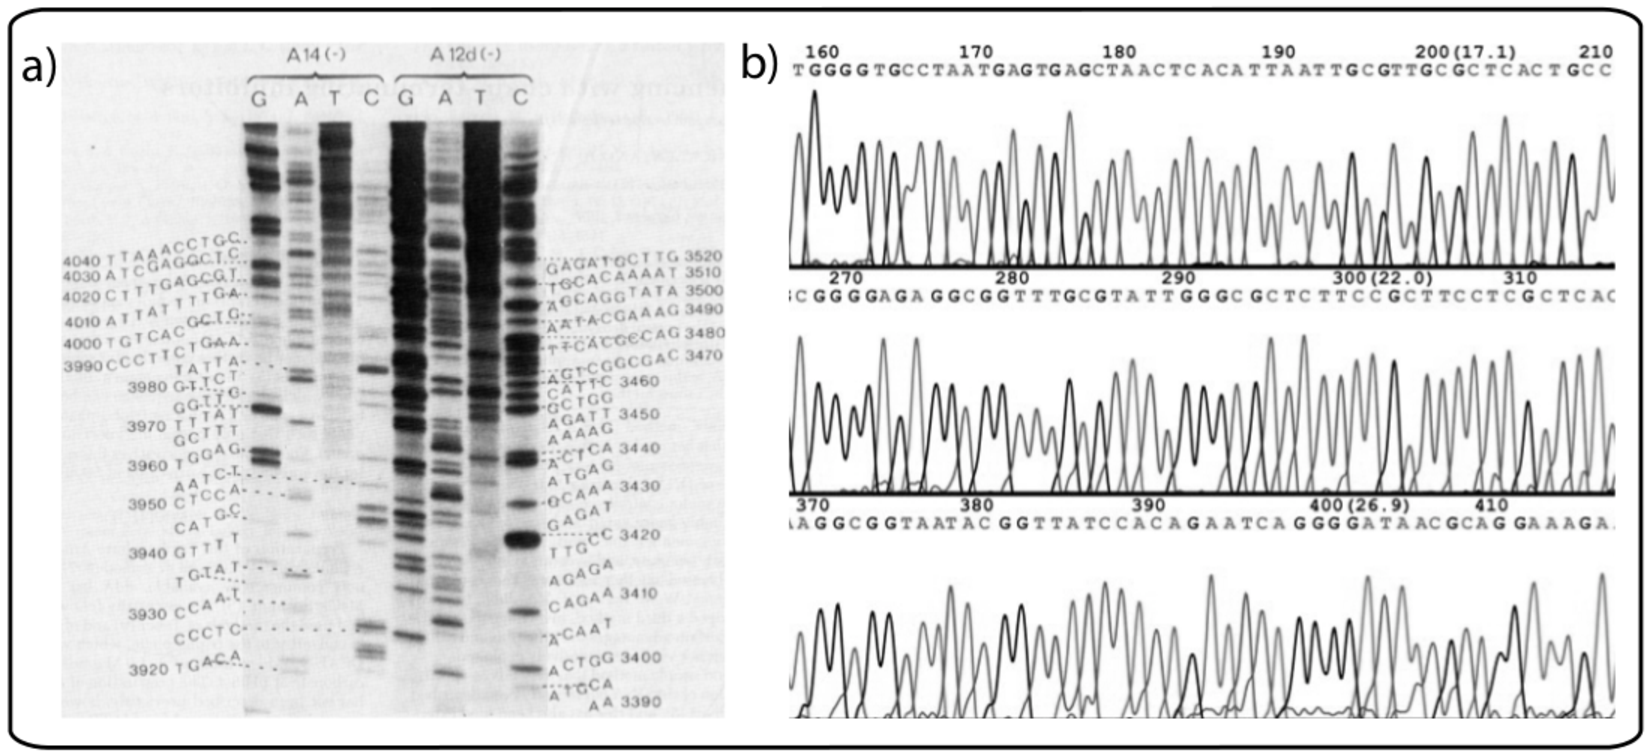
\includegraphics[width=1\textwidth]{figures/Introduction/thesis_1}
	\caption{\label{fig:sanger}\textbf{Evolution of Sanger sequencing}\\
			a) Autoradiograph of an acrylamide gel \cite{sanger1977dna} \\
			b) Electropherogram of a dye terminator sequencing, separated by capillar electrophoresis \cite{electropherogram}}
\end{figure}

The first method to be successfully adopted for DNA sequencing was developed by Sanger and colleagues (\cite{Sanger1975441} and \cite{sanger1977dna}) and is known as chain-termination sequencing: the single strand template is replicated using the enzyme DNA-polymerase and a set of nucleotides containing a certain amount of dideoxynucleotidetriphosphates (ddNTPs), which cause a termination in the DNA synthesis. During the next 40 years this technique has been refined, changing from the initial manual procedure using four different reactions with radioactive-labeled ddNTPs and a gel electrophoresis to the dye-terminator technology, in which the ddNTPs are labeled with a different fluorescent dye and the resulting fragments are separated by capillary electrophoresis and read with a laser (Figure \ref{fig:sanger}): this advances lead to the automation of the whole sequencing process, with a drop in cost and time needed. Thanks to this technological advances, it was no longer impossible to obtain the complete DNA sequence of an organism, at any phylogenetic scale: in fact, even if the first genomic sequences belonged to viruses \cite{sanger1978nucleotide} and small bacteria \cite{fleischmann1995whole}, the important contribution of computational techniques of the young field of bioinformatics helped in obtaining the genomic sequences of higher organisms such as yeast (\textit{Saccharomices cerevisiae}, \cite{goffeau1996life}), the nematode \textit{Caenorhabditis elegans} \cite{caenorhabditis1998genome}, the fruit fly (\textit{Drosophila melanogaster}, \cite{adams2000genome}) and of course the human genome (\cite{lander2001initial} and \cite{venter2001sequence}).

If this shift from a gene-centric to a genome-centric perspective made possible to study the whole repertoire of the genetic elements present in a given species, on the other hand a new challenge was immediately posed: the growing quantity of data produced (i.e. sequences) needed to be handled properly, since each fragment that is sequenced has a limited length and therefore needs to be tied together, and the genetic features have to be found inside the sequence. To overcome this new challenges that arose with the new sequencing technologies, the field of bioinformatics (also known as computational biology) was born: the biological sequences could then be encoded in a computer-friendly way and a series of algorithms that model biological processes could be created and applied to these sequences.

\subsection{From raw sequences to predicted functions}
In order to obtain a complete genome sequence of an organism, including the information regarding the position and function of each gene, a number of computational steps have to be applied, each one with different problems and constraints: with the evolution of sequencing technologies, the number of algorithms and softwares designed to address each one of the steps needed to obtain an annotated genomic sequence has increased.

\subsubsection*{Sequence trimming}
The first step in the sequence management directly involves the reads produces by the sequencing machine, which are short sequence fragments, and which strongly influences the following steps; disregard of the detection technology, each position is assigned to a base with an error probability. Since the sequence quality usually drops towards the read's end, it is important to remove the bases with higher error probability from the end of the sequence read, in order to ensure an accurate sequence; this process is known as \textit{trimming}. Trimming methods mostly rely on a particular quality encoding defined by the Phred program \cite{ewing1998base}\cite{ewing1998base2}, in which the quality score is logarithmically proportional to the base-call error probability (Equation \ref{eq:phred}); this quality measure has been encoded as ASCII characters together with the putative sequence in the FASTQ file format \cite{cock2010sanger}. 

\begin{equation}
\label{eq:phred}
Q = -10 \log_{10}P
\end{equation}

Usually a window approach is used to scan each read and discard those regions with poor quality (usually with Phred quality 30 or below, which corresponds to a base call accuracy of 99\%).

\subsubsection*{Assembly}
\label{sec:hamiltonian}
Once that the reads have been trimmed to remove low quality bases, the next task is to merge the short reads into larger sequences, which possibly can lead to reconstruct the whole target genome: the process is called \textit{assembly}; the adopted strategy strongly depends on the reads length, on the number of repetitions and sequence coverage, which can vary with each genome; in this paragraph only the approach used in sanger sequencing project is considered: the other algorithms will be discussed in section \ref{sec:revolution}. The core of each algorithm developed to assembly Sanger sequences relies on the measure of overlaps between the reads and the construction of a directed graph in which the nodes represent each read and the edges alignments between reads passing an arbitrary set of cut-offs: the final sequence is then reconstructed by looking for an Hamiltonian cycle inside this directed graph (Figure \ref{fig:assembly}) \cite{compeau2011apply}. The efficiency of this algorithm is mainly reduced for the presence of duplicated sequence, which is often the case, especially for bacterial genomes rich in trasposable elements; the research of Hamiltonian cycles inside the constructed graph is also a limit, since all the pairwise alignments between reads have to be constructed: these limitations have been addressed in many assemblers \cite{myers2000whole}\cite{batzoglou2002arachne}.
Given this limitations, a complete genome sequence cannot be obtained with such approaches; instead, a variable number of contiguos sequences (called \textit{contigs}) are obtained, whose length is dependent on reads length and quality and on the number of duplicated sequences in the genome. The gaps between each contig can be closed in the so-called \textit{finishing} phase, in which a series of PCR reactions are designed between pair of contigs that are thought to be adjacent, based on physical maps or other biological data.

\begin{figure}[!tb]
	\center
    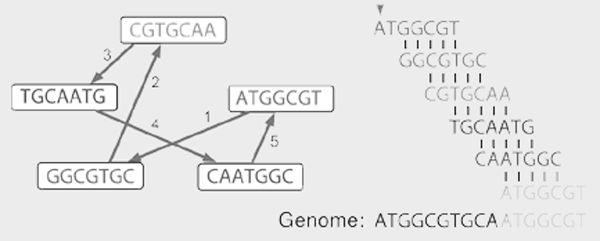
\includegraphics[width=0.66\textwidth]{figures/Introduction/thesis_2}
	\caption{\label{fig:assembly}\textbf{Assembly of Sanger sequences}\\
			(from \cite{compeau2011apply})}
\end{figure}

\subsubsection*{Annotation (I): gene calling}
Once that sequences with satisfactory length are obtained, the position of the ORFs (and other regulatory features) has to be extracted from the plain sequence: this process is known either with the term \textit{annotation} or \textit{gene calling}. Since experimental approaches are not affordable in term of time and cost, predictions have to be made to annotate the obtained sequence, taking advantage of the mechanisms of transcription and traduction and sets of experimentally validated gene annotations. The start codons are known to be ATG, GTG and TTG (especially in bacteria): given a random nucleotide sequence, we expect to find a stop codon every 60bp (5\% probability); however, it is known from the experiments that the average bacterial gene length is around 300bp. A first naive method would be then to find all the ORFs with length over 60bp: which indeed is the first step in many gene-calling softwares (see for instance prodigal \cite{hyatt2010prodigal}); however, the assumption that a genomic sequence has a random distribution is off course false, since each bacterial genomes has a distinct GC content, a distinct codon usage \cite{ermolaeva2001synonymous}, different intergenic regions sizes and the presence of signal sequences like the RBS: each bacterial species will therefore have a distinct gene signature. Gene calling algorithms take into account this species specific bias by using statistical models (like HMMs) and dynamic programming approaches, together classified under the name of \textit{ab initio} methods \cite{do2006computational}. 

\subsubsection*{Annotation (II): function assignement}
\begin{figure}[!tb]
	\center
    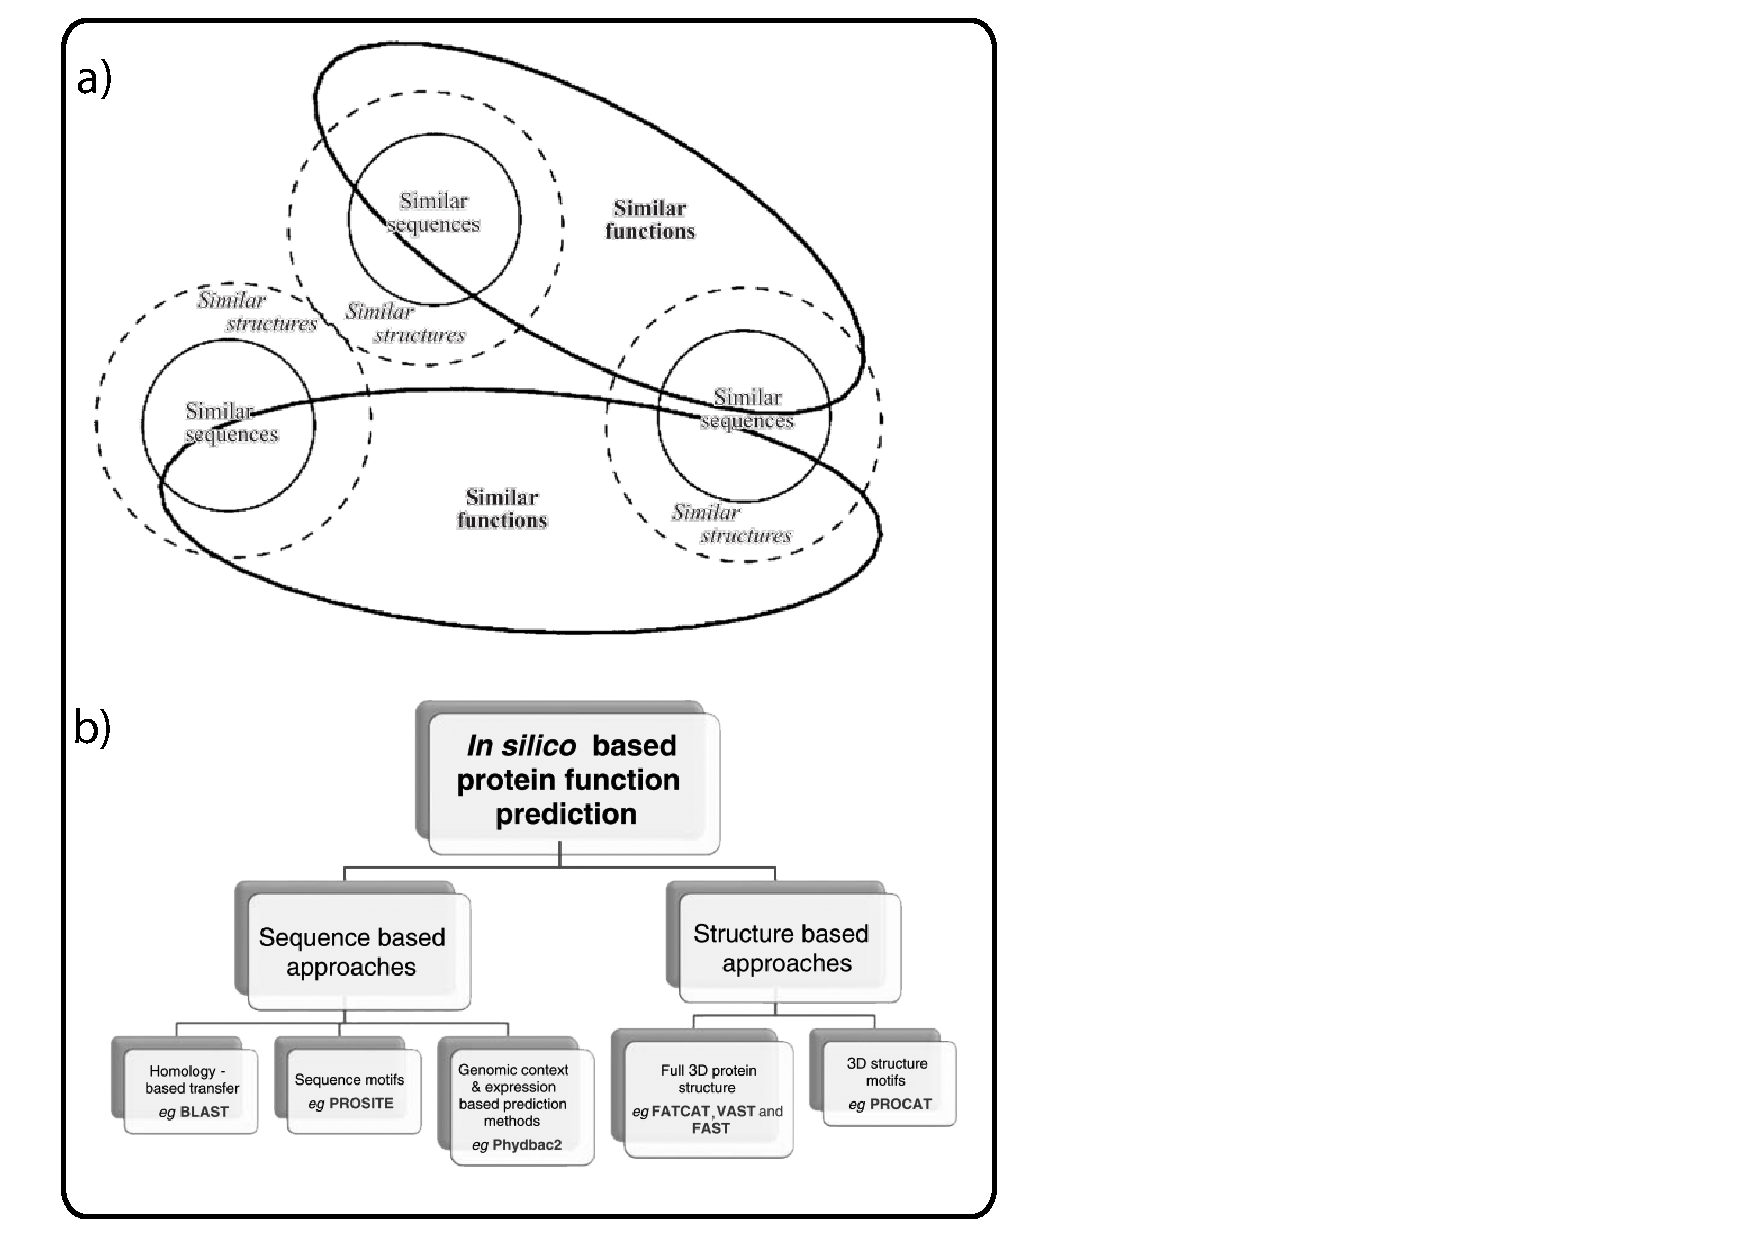
\includegraphics[width=0.66\textwidth]{figures/Introduction/thesis_3}
	\caption{\label{fig:funcannotation}\textbf{Functional annotation}\\
			a) Different patterns of functional similarity (from \cite{whisstock2003prediction}) \\
			b) Overview of functional annotation techniques (from \cite{sleator2010overview})}
\end{figure}

Given the high number of proteins that are annotated in each bacterial genome, experimental strategies to depict the function of each gene are not affordable; bioinformatic analyses are used instead, lead by the principle that proteins that exhibit a certain degree of similarity are probably evolutionary related and therefore should share similar functional features. This similarity can be measured at different levels: at the sequence level (through a BLAST \cite{camacho2009blast+} search on public databases) or at the structural level, which in some cases may be equivalent (Figure \ref{fig:funcannotation}a); the major problems in this transfer of function through homology is that there are no defined thresholds for this similarity measures and, most importantly, even closely similar sequences may exhibit very different functions. An important conseguence of this incorrect annotations is that the errors are propagated through each new sequenced genome in which a protein with enough similarity to the wrongly annotated protein is found \cite{whisstock2003prediction} \cite{sleator2010overview}. To overcome this problems, a series of alternative strategies have been developed: the use of curated protein databases (such as KEGG \cite{ogata1999kegg}) ensure a reduction of annotation errors and allows a partial metabolism reconstruction; the research of sequence motifs and domains instead of using the whole sequence allows a more granular and precise functional reconstruction, focusing on functional modules, which are less prone to ambiguations (see for instance INTERPRO \cite{apweiler2001interpro}\cite{zdobnov2001interproscan}) and, especially for bacterial genomes, the information about genomic context can be used to infer the function of a protein based on the known operons and genomic islands \cite{sleator2010overview} (Figure \ref{fig:funcannotation}b). All these automatic annotation methods are often refined by careful manual curators (i.e. as in the UNIPROT database \cite{uniprot2008universal}), which often take advantage of functional ontologies like GO \cite{ashburner2000gene} and experiments from the literature to better refine and correct the automatic annotations.

%HERE EXPAND WITH MORE DETAILS ON THE VARIOUS ANNOTATION TECHNIQUES?

\subsection{Bacterial genomics}
\label{sec:genemining}
Compared to partial sequences, complete (or even draft) genomic sequences allowed a wider array of analysis on a particular species: in fact, since all the functional repertoire of an organism is encoded in the genome, a complete reconstruction of the functions of an organism was theoretically possible, thanks to the functional annotation techniques described above; various analyses that were previously impossible have been made available thanks to bacterial genomics.

The presence of single genes or functions of interest could be easily tested looking for an homolog of an evolutionary related gene with known sequence; however, similar biological functions can belong to two proteins even if there is no evolutionary relationship (a phenomenon known as \textit{convergent evolution}), so the presence of a particular function must be checked by taking into account other sources of information, like the presence of a reaction in the metabolic network reconstruction (i.e. through KEGG), or the presence of a certain protein domain or the combination of two or more domains (i.e. through INTERPRO) in a gene, with the methods described above. This \textit{in-silico} approaches are often been referred as \textit{gene-mining} \cite{li2004gene}\cite{du2008functional}, which could help to reduce the amount of experiments needed to test the phenotype of an organism and the presence of a particular gene.

The potentials of bacterial genomics, however, are not limited to the analysis of a single gene or function, but indeed have been expanded to allow a broader and more general functional description of a bacterial species. One of the most powerful method that has been developed is based on the utilization of a controlled vocabulary (also termed as \textit{ontology}) of gene functions, divided in three macro-categories and with a hierarchical structure, with an increasing level of detail (Figure \ref{fig:gocog}a); this annotation categorization method is called the Gene Ontology \cite{ashburner2000gene}, and even if it was developed for eukaryotic species, it can also be applied to the bacterial kingdom. The three macro-categories were designed to address all the functional aspects of a gene product:

\begin{itemize}
\item \textbf{Biological process} is used to describe the biological objective of a gene: examples may be GO:0048591 (cellular growth) or GO:0009758 (carbohydrate utilization),
\item \textbf{Molecular function} describes the 	biochemical activity of a gene, including physical interactions: examples may be GO:0016874 (ligase activity) and GO:0003989 (acetyl-CoA carboxylase activity),
\item \textbf{Cellular component} describes where the function of the gene is expressed, a description that is more variable for eukaryotes than in bacteria: examples may be GO:0016020 (membrane) and GO:0043190 (ATP-binding cassette (ABC) transporter complex).
\end{itemize}

\begin{figure}[!tb]
	\center
    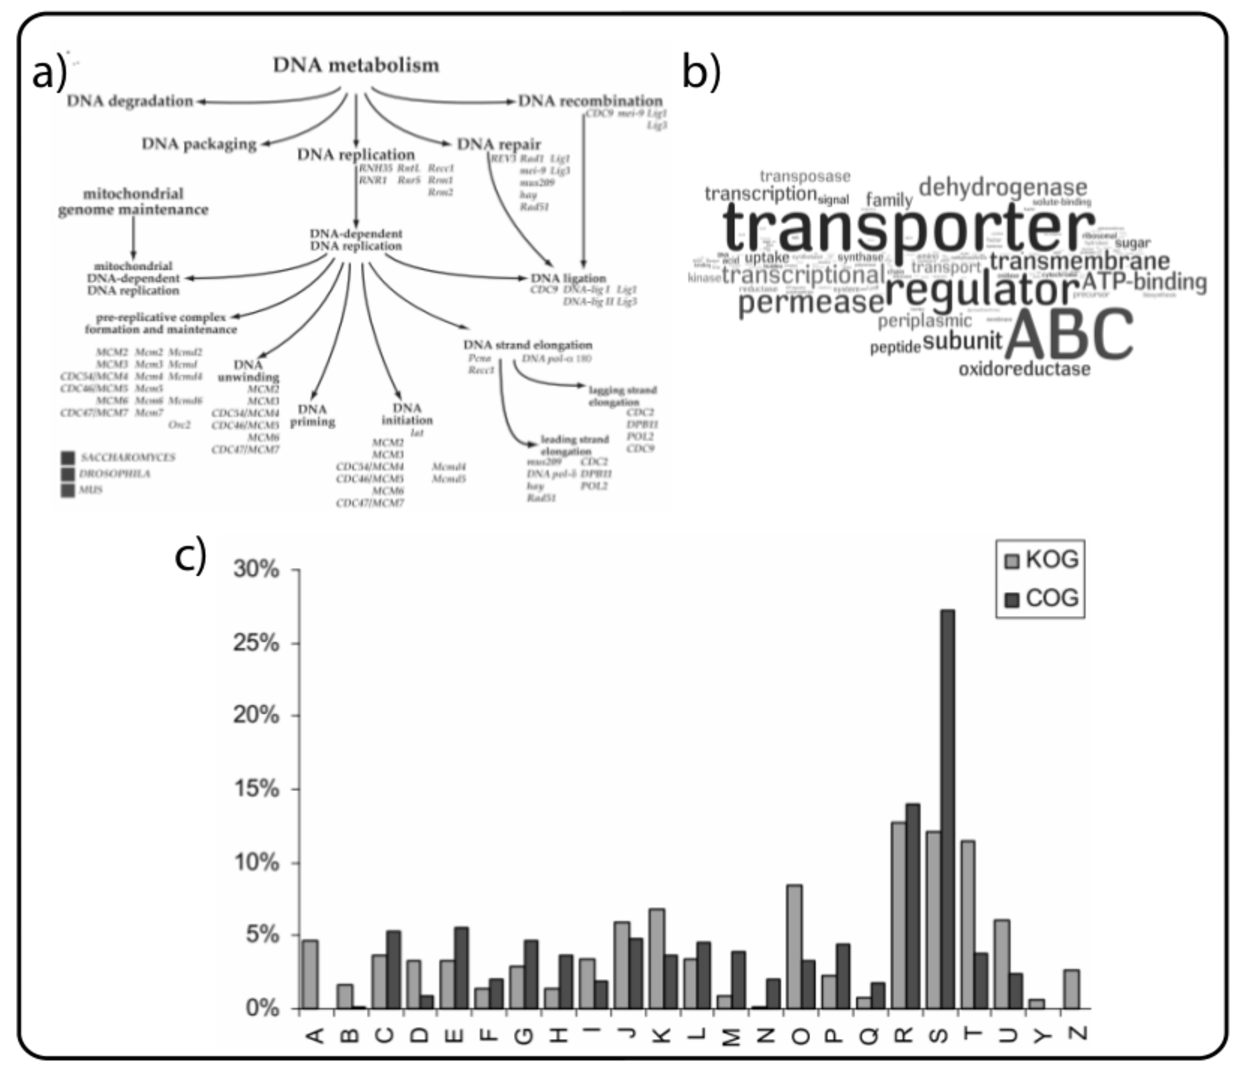
\includegraphics[width=0.77\textwidth]{figures/Introduction/thesis_4}
	\caption{\label{fig:gocog}\textbf{Functional categories}\\
			a) Example of the hierarchical structure of a GO annotation (from \cite{ashburner2000gene}) \\
			b) Word cloud of all the annotation terms found in \textit{S. meliloti} Rm1021; the size of each word is proportional to the frequency of the term (from \cite{wordcloud}) \\
			c) Broad functional categorization of prokaryotes (COG) and eukaryotes (KOG) (from \cite{tatusov2003cog})}
\end{figure}

The hierarchical structure of the gene ontology, with increasing levels of details allowed a precise and granular functional categorization of gene products, given the amount of experimental and predicted information available; most importantly, the ontologies can be updated with the results of new experiments and other evidences. Since all the proteins from a genome can be annotated using this method, an important consequence is that it is possible to construct an overall functional categorization of a given species (Figure \ref{fig:gocog}b), with the possibility to obtain a first general functional categorization of a species, which can be later compared to other organisms. The same approach can be applied using another annotation method with a general functional categorization, called COG \cite{tatusov1997genomic}\cite{tatusov2003cog}, which is a set of orthologs from all the three kingdoms of life (the current version has been built upon 66 genomes \cite{cogcategs}), each one belonging to one of the 25 macro-categories, further divided into single orthologs with a more precise functional categorization. Each protein can be assigned to a COG using rps-blast (reverse position specific blast) \cite{a1999impala}\cite{marchler2002cdd}, which allows to query a sequence against a library of position-specific scoring matrices (PSSMs) derived from each COG, thus assigning each protein to one (or more) COG categories; it is therefore possible to obtain a functional insight of the whole genome (with a lower degree of complexity, compared with GO), which again can be compared to other organisms (Figure \ref{fig:gocog}c).

\newpage
\section{From genomics to comparative genomics}
Describing the bacterial genomics as a series of analysis on a single organisms is indeed a rather big simplification: in fact, from the very beginning of the bacterial genomics era, questions regarding the genomic evolution were posed; the term \textit{comparative genomics} appeared then as soon as two bacterial genomes were available \cite{koonin1996complete}. Given that all life forms may have evolved from a last universal common ancestor (LUCA \cite{delaye2005last}\cite{koonin2005origin}), it is obvious to assume that many genes may be shared in all the three kingdoms of life, and in particular in the bacterial kingdom; the main goal is to understand which fraction of the genome is evolutionary conserved, which genetic traits have evolved through convergent evolution, and which genetic elements are specific to a particular taxa or to a single species. One of the most interesting questions that can be addressed through evolutionary comparative genomics is the analysis of the so-called \textit{minimal genome}, which theoretically is the minimum gene set able to support life; such a gene set should be present in all life forms, with genes involved in the replication of the genetic material, cell division and the core metabolism. Evidences of the presence of the minimal genome has been found already at the beginning of the genomics era, and more recent works have refined its putative size and gene content to about 200 genes \cite{koonin1996complete}\cite{koonin1996sequencing}\cite{gibson2008complete}.

%Comparative genomics is off course not only limited to evolutionary studies, but as soon as more genomes were available, was expanded to include other functional approaches (EXPAND OR REMOVE)

\subsection{Transferring functions: homologs, orthologs and paralogs}
The core foundation of comparative genomics analyses is the definition of the list of orthologs between two or more species: this term has seen many definitions during the recent history of biological science, which change significantly its biological meaning and the methods for its assesment \cite{altenhoff2009phylogenetic}. The first definition was given by Fitch in 1970 \cite{fitch1970distinguishing}, indicating those genes that have diverged through a speciation event; another, more practical definition of orthology is about function, as two orthologs are considered to exhibit the same function. The functional definition of orthology has an important consequence: annotations can be transferred from one genome to another when the orthologs are defined, thus avoiding the need for experimental validations of functions; most importantly, two genomes can be easily compared to highlight functional differences. However, since the lack for an univocal definition of protein function, this approach has to be taken with caution to avoid propagations of incorrect annotations, as well as a series of directed experiments to validate the transferred functional annotation. Another important feature of orthologous relationships is that the orthology information is not transitive, meaning that if a third protein has to be added to an existing pair of orthologs, each pairwise analysis has to be conducted separately \cite{altenhoff2009phylogenetic}.

%USE OF ORTHOLOGS IN C:GENOMICS?
\subsubsection{Orthologs and paralogs}
\begin{figure}[!tb]
	\center
    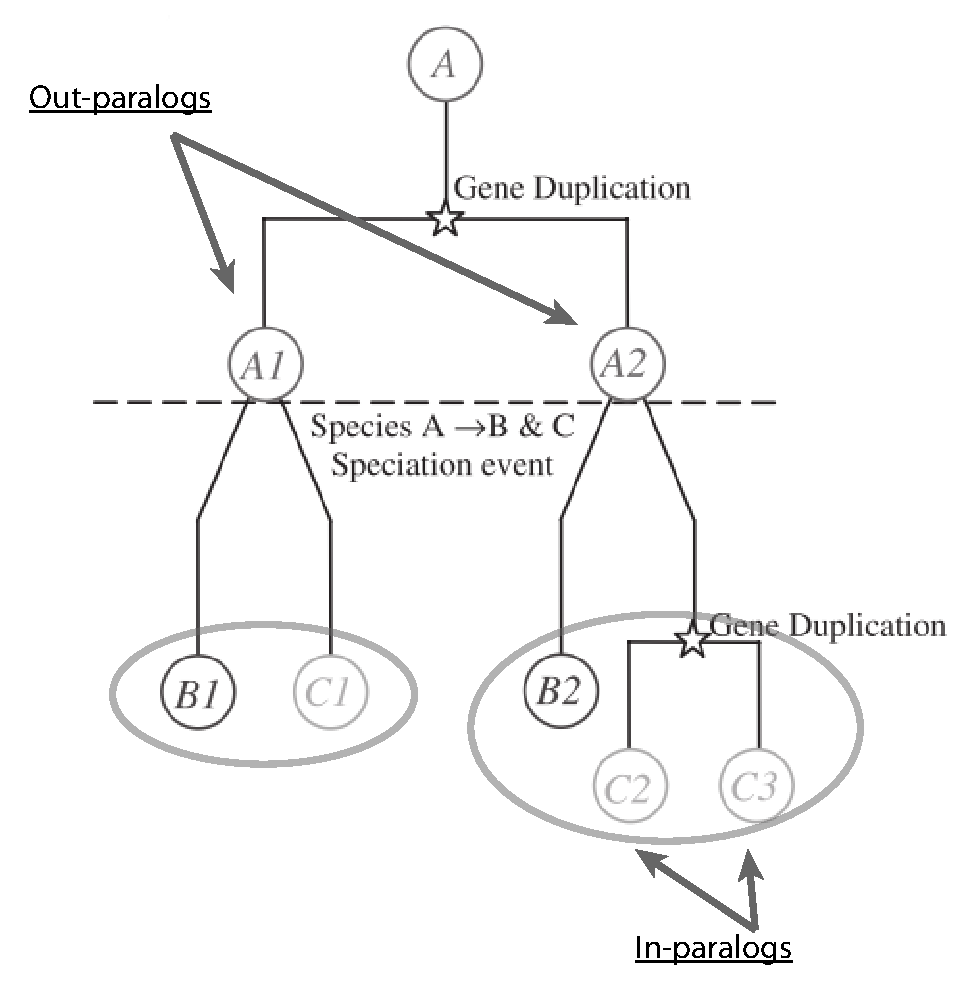
\includegraphics[width=0.77\textwidth]{figures/Introduction/thesis_5}
	\caption{\label{fig:orthologs}\textbf{Orthologs and paralogs}\\
			Distinction between out-paralogs and in-paralogs; grey elipses indicate orthologs (modified from \cite{o2005inparanoid})}
\end{figure}
Since the evolution of bacterial genomes doesn't rely only on mutations at the single nucleotide level, but instead consists also of recombinations, deletions and duplications, an additional category of orthologs (\textit{paralogs}) has to be considered to include gene duplication events: they are, in theory \textit{bona-fide} orthologs as the original copy. An important distinction however has to be made, since several examples in eukaryotes have shown that some paralogs have diverged so much from the original copy to the point were the function is significantly altered \cite{studer2009confident}\cite{nehrt2011testing}; the proposed distinction is between \textit{out}-paralogs, whose duplication events occurred before the speciation event, and \textit{in}-paralogs, whose duplication occurred after the speciation event \cite{remm2001automatic} (Figure \ref{fig:orthologs}). Out-paralogs, although retaining a significant degree of homology and a putative similar function, are not to be considered orthologs, while the in-paralogs are most likely to retain the same function.

\subsubsection{Algorithms to infer orthology}
Many algorithms have been developed for the assessment of orthology, and many of them have been scaled up to allow the analysis on whole genomic sequences: they can be roughly divided in two main categories, according to the main source of information for the orthology calling (Table \ref{tab:orthologs}).

\begin{table}
    \begin{tabularx}{\textwidth}{|p{2.9cm}|p{5.3cm}|p{3.6cm}|}
        \hline
        \textbf{Method} & \textbf{Features} & \textbf{Examples} \\ \hline
        Tree based & Construction of phylogenetic trees, followed by reconciliation with species tree & Ensembl compara \cite{kersey2010ensembl}, LOFT \cite{van2007orthology}, TreeFam \cite{li2006treefam} \\ 
        Homology based & Sequence similarity measures, followed by clusterization techniques & BBH, COG/KOG \cite{tatusov1997genomic}\cite{tatusov2003cog}, InParanoid \cite{o2005inparanoid} \& Multiparanoid \cite{alexeyenko2006automatic}, OrthoMCL \cite{li2003orthomcl}, EggNOG \cite{jensen2008eggnog} \\ 
        Other & Pairwise evolutionary distances, reciprocal smaller distances, gene context conservation & RoundUp \cite{deluca2006roundup}, Homologene \cite{wheeler2007database}, OMA \cite{dessimoz2005oma} \\
        \hline
    \end{tabularx}
	\caption{\label{tab:orthologs}\textbf{Overview of orthology assesment methods}}
\end{table}

\paragraph{Tree based}
The first method to be implemented was based on the construction of a multiple sequence alignment tree and its comparison with the analyzed species tree to infer the orthologs clusters, a method called \textit{reconciliation}. Although this method has proven to be precise, it's extremely time consuming, since it usually requires a manual curation step to resolve the tree conflicts, so it's usually used for small gene families; moreover, horizontal gene transfer events (HGT) may alter the sequence tree topology, rendering this method particularly tricky for bacterial genomes, where HGT is very common.

\paragraph{Homology based}
The presence of complete bacterial genomes has led to the development of new automatic methods for orthology assesment, which allow the analysis of whole bacterial genomes in a reasonable amount of time; these methods are based on homology measures (since orthologs are also homologs, even though the contrary is not necessarily true \cite{altenhoff2009phylogenetic}), which lead to the definition of an homology matrix between each protein pair that has then to be clusterized to extract the orthologs. These methods are characterized by an higher number of false positives, because of events such as gene losses, but can work even for big phylogenetic distances. Most of the algorithms based on this method use Blast for the homology measure, with different clusterization methods. The most simple implementation of this method is the so-called Bidirectional Best Hit (BBH, Figure \ref{fig:bbh}): the orthologs of genome A are defined as those proteins whose best match in genome B have the same protein as best match in genome A. All the other algorithms rely on this concept, while changing the various filters and clusterization steps: InParanoid for instance allows the definition of paralogs, which cannot automatically be defined by naive BBH algorithms.

\begin{figure}[!tb]
	\center
    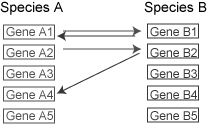
\includegraphics[width=0.5\textwidth]{figures/Introduction/thesis_6}
	\caption{\label{fig:bbh}\textbf{BBH algorithm}\\
			Schematic function of the BBH algorithm: the first two proteins are orthologs, the other three are just homologs (from \cite{bbh})}
\end{figure}

\subsection{The revolution in sequencing technologies}
\label{sec:revolution}
The last decade has seen a series of impressive developments in automatic sequencing technologies, with the creation of many new techniques and platforms: compared to the first era of genomes sequencing, biologists now can decide which technology is best suited for their analysis. All these new developments have been termed \textit{Next-generation Sequencing} (NGS), including also the latest automatic Sanger sequencing technologies \cite{glenn2011field}; even though there are many platforms available, the NGS technologies are usually divided in three distinct generations, according to their peculiarities:

\begin{itemize}
\item \textbf{1\textsuperscript{st} generation:} capillary Sanger sequencing through dye-terminator,
\item \textbf{2\textsuperscript{nd} generation:} platforms that require amplification of the template sequence prior to the sequencing step,
\item \textbf{3\textsuperscript{rd} generation:} platforms that directly sequence individual DNA molecules.
\end{itemize}

Even if the first reports about the NGS techniques are dated in 1996 \cite{ronaghi1996real}, the first commercial applications of the pyrosequencing technologies appeared in 2005; since then, each year has seen the development of new instruments and variations, with a considerable drop in the cost/Mb. The major platforms used today are listed below (Table \ref{tab:ngs}, Figure \ref{fig:ngs}).

\begin{table}
    \begin{tabularx}{\textwidth}{|p{2cm}|p{5.3cm}|p{2.8cm}|p{1.2cm}|}
        \hline
        Platform    & Sequencing method          & Amplification method & Reads-length \\ \hline
        454         & Synthesis (pyrosequencing) & emPCR                & 400-700      \\ 
        Illumina    & Synthesis                  & BridgePCR            & 100          \\ 
        SOLiD       & Ligation                   & emPCR                & 35-75        \\ 
        HeliScope   & Synthesis                  & ~                    & 35           \\ 
        Ion Torrent & Synthesis (H\textsuperscript{+} detection)   & emPCR                & 100         \\ 
        PacBio      & Synthesis                  & ~                    & 860-1100     \\
        \hline
    \end{tabularx}
    \caption{\label{tab:ngs}\textbf{Overview on NGS sequencing platforms} (adapted from \cite{glenn2011field})}
\end{table}

\paragraph{454} The first NGS technology to be implemented, in which single template molecules are amplified through \textit{emPCR} (emulsion PCR), a technique in which each DNA molecule is trapped inside aqueous droplets together with a primer-coated bead and the PCR reagents; later each bead is trapped inside a picotitre plate designed to contain exactly one bead for well. The sequence is then read through pyrosequencing: a dNTP is added on the plate, together with the enzymes DNA polymerase, ATP sulfurylase, luciferase and apyrase, and with the substrates adenosine 5'  phosphosulfate (APS) and luciferin; the incorporation of a dNTP releases pyrophosphate, which is converted, together with adenosine 5' phosphosulfate, into ATP by the enzyme ATP sulfurylase: the ATP is then used by the luciferase to convert luciferin to oxyluciferin that generates light. The amount of light emitted by each well is directly proportional to the number of bases that were incorporated by the DNA polymerase.

\paragraph{Illumina} Formerly known as Solexa, this technology is based on the adhesion of the template sequences to a special glass surface with a series of single-strand primers complementary to the adaptors ligated to the templates; the single templates are amplified through \textit{Bridge PCR}, obtaining a series of clusters containing many copies of the same template. Sequencing is achieved through the contemporary addiction of four dNTPs labelled with fluorescent dyes, which are read with a camera. Compared with 454, Illumina reads are usually shorter, but with an higher sequencing depth.

\paragraph{SOLiD} Unlike the previous platforms, the SOLiD technology obtains the sequences through ligation, instead of synthesis; the template preparation is similar to 454, with emPCR apmlification on beads, ligated to a glass surface. The actual sequencing step involves the utilization of all the possible di-NTPs, each one labeled with a different fluorescent dye; many different cycles involving different primers are used, leading to a double reading of each base. This technology yields reads that are significantly shorter than the others, but with an higher accuracy and depth.

\paragraph{HeliScope} The first single-molecule sequencing platform to be developed, performs sequencing through the addiction of each fluorescently labeled dNTP and the subsequent read through a laser camera. Read sizes are comparable to the SOLiD platform.

\begin{figure}[!htb]
	\center
    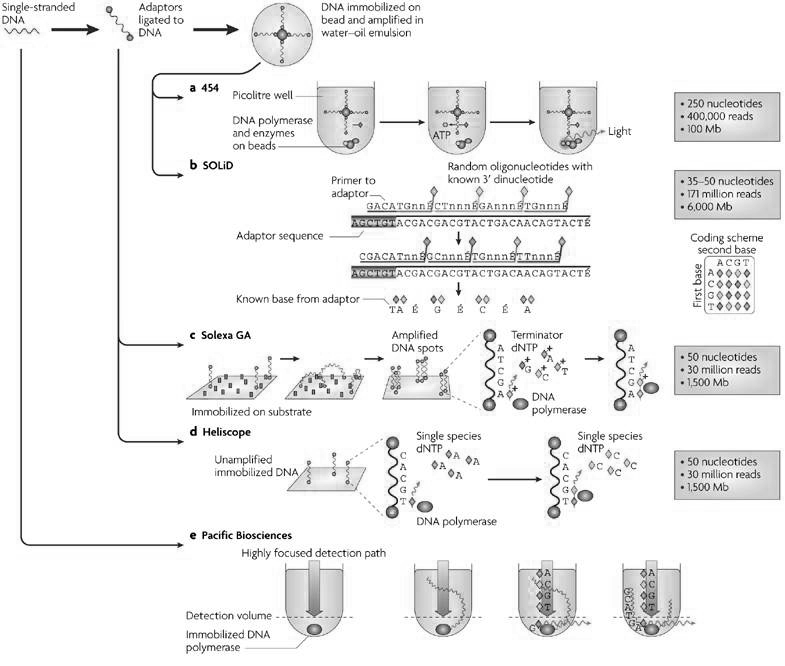
\includegraphics[width=1\textwidth]{figures/Introduction/thesis_7}
	\caption{\label{fig:ngs}\textbf{NGS overview}\\
			Main features of the NGS technologies, except the Ion Torrent platform (from \cite{maclean2009application})}
\end{figure}

\paragraph{Ion Torrent} This platform has the distinctive feature, compared the the others: it doesn't need a camera for the recognition of the incorporated dNTPs, thus reducing the size of the corresponding apparatus and increasing the speed of the analysis. In this technique, each DNA molecule is incorporated in a well inside a semiconductor chip, together with the enzyme DNA polymerase: the dNTPs are added sequentially, with the release of a proton when the nucleotide is incorporated, which is detected by an ion sensor. The amount of electronic signal is directly proportional to the number of dNTPs that have been added to the growing strand (Figure \ref{fig:ion}). 

\begin{figure}[!b]
	\center
    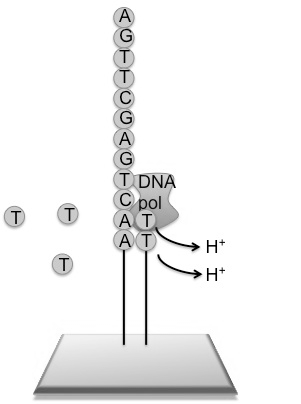
\includegraphics[width=0.33\textwidth]{figures/Introduction/thesis_8}
	\caption{\label{fig:ion}\textbf{Ion Torrent technology}\\
			Schematic function of the Ion Torrent sequencing by synthesis with proton detection (from \cite{ion})}
\end{figure}

\paragraph{PacBio} This technology is also known as single molecule real time sequencing, in which single DNA molecules are present inside microscopic wells, with a molecule of the enzyme DNA polymerase at the bottom; each fluorescent dNTP is added sequentially, and its incorporation is detected through a camera: a single nucleotide incorporation can be detected, thanks to the use of zero-mode waveguide wells, which confer particular properties to light \cite{eid2009real}. Compared to the other NGS sequencing technologies, this platform allows reads with mean length of about 1000bp, comparable to Sanger sequencing.

\begin{figure}[!htb]
	\center
    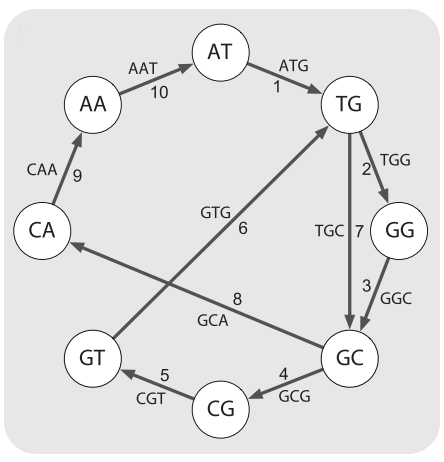
\includegraphics[width=0.7\textwidth]{figures/Introduction/thesis_9}
	\caption{\label{fig:debrujin}\textbf{Assembly through de Brujin graphs}\\
			Schematic representation of a de Brujin graph with k-size 3 (from \cite{compeau2011apply})}
\end{figure}

Compared to tradional Sanger sequencing (section \ref{sec:hamiltonian}), the amount of sequences produced by the NGS technologies (especially for Illumina), poses serious problems for genome assembly through hamiltonian cycles algorithm, whose efficiency is strongly reduced also by the relatively low average length of the reads, with the need to perform a really high number of alignments (in fact, this algorithm is \textit{NP-complete}, meaning that an optimal solution for this problem may not exists). These limitations have been addressed in NGS sequences assembly with the adoption of the so-called \textit{de Brujin} graphs \cite{compeau2011apply}: the graph is constructed with the adoption of sequences \textit{k-mers} (with k values usually below half of the average read length). Each node of the graph is composed by all the k-1 mers that are found in the reads pool, with an edge between two nodes if exists a k-mer that has two nodes as prefix and suffix (Figure \ref{fig:debrujin}); the assembly is then obtained through an eulerian cycle search, that is a cycle in which each edge is visited exactly once, an algorithm approach with reduced complexity. The same problems as hamiltonian algorithms are off course still present, like the presence of duplicated sequences, but many assemblers have already been developed to solve these problems \cite{simpson2009abyss}\cite{boisvert2010ray}\cite{zerbino2008velvet}. 

\subsection{One species, many sequences}
\begin{figure}[!tb]
	\center
    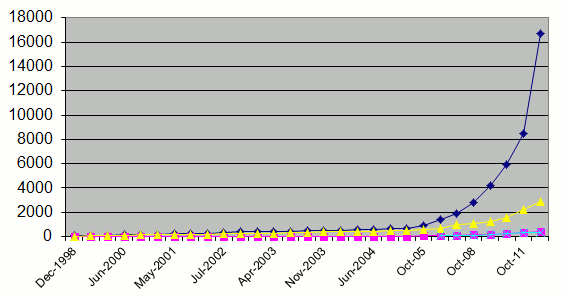
\includegraphics[width=1\textwidth]{figures/Introduction/thesis_10}
	\caption{\label{fig:gold}\textbf{Genome projects according to phylogenetic group }\\
			Number of genome projects registered in the GOLD database, October 2012 (from \cite{gold}). Blu line, bacteria; pink line, archea; yellow line, eukarya; cyan line, mammals.}
\end{figure}

The proliferation of such an high number of new sequencing technologies, each one in competition with the others, has lead to a dramatic drop in the complete genomic sequencing costs, leading to the definition of new terms and of the comparative genomics analysis. The first tangible conseguence is the higher number of genomic sequences that are added to public databases each year, with a prominent role of bacterial species, which outnumber any other taxonomical group (Figure \ref{fig:gold}); in fact the number of available bacterial genomic sequences in the NCBI repository are 2171 (on November 2012), with many more sequences available each day, as all the genome projects are closed and the data submitted. Not all these new projects and sequences belong to distinct species, but in many cases many genomes for each species are available (Figure \ref{fig:intraspecies}). The term comparative genomics was then expanded to include those analysis between genomes coming from the same species, with important functional and evolutionary applications.

\begin{figure}[!tb]
	\center
    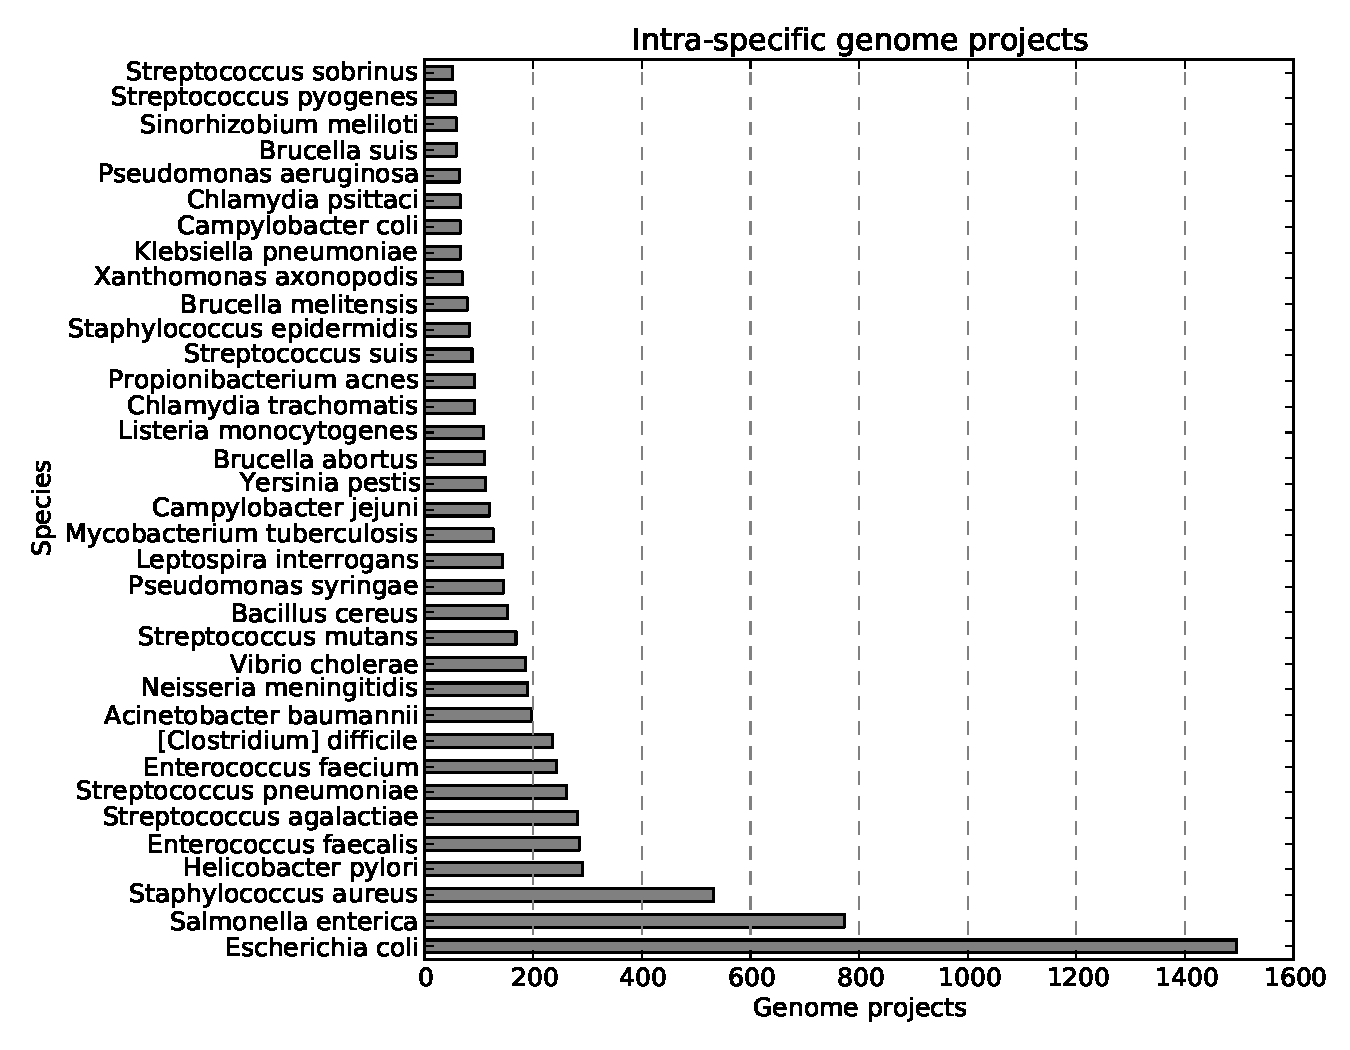
\includegraphics[width=1\textwidth]{figures/Introduction/thesis_11}
	\caption{\label{fig:intraspecies}\textbf{Bacterial species with more than 50 genomic projects}\\
			Number of genome projects registered in the GOLD database, October 2012 (from \cite{gold}).}
\end{figure}

\subsection{Intra-specific comparative genomics}
The species concept is challenged by the bacterial world, since a morphological and functional categorization of a bacterial species is not defined and certain, and also genetically, the low barriers on genetic exchange between bacteria (HGT events, transduction, transformation, ecc.) poses serious doubts on the application of the species label to a bacterial entity, even though markers such as the 16s rRNA can still be used. Given the high functional variability inside a so-called bacterial \textit{species}, interesting questions have been posed on which fractions are conserved and which ones are variable inside a genome and how it evolves inside a species. The strategies to address these question involve the genome comparison, through the definition of all the orthologous groups inside a genome, in order to highlight those genes that are common to all the analyzed strains and those that are specific to one or more strains: the whole orthologous groups set inside a set of genomes has been termed \textit{pan-genome}, after the observation that new genes are always discovered when a new genome of a particular species is sequenced \cite{tettelin2005genome}\cite{medini2005microbial}. The pangenome could be therefore used to describe the overall functional repertoire of a species, and most importantly to define the dynamics of acquisition and loss of such functions.

\subsubsection{Core, accessory and unique genome}
The orthologous groups that are part of a microbial pangenome can be further divided in other catogories, according to their occurrence in the analyzed strains:

\begin{itemize}
\item \textbf{Core genome:} orthologs that are present in each genome,
\item \textbf{Dispensable genome:} orthologs that are present in one or more genomes, but not in all,
	\begin{itemize}
		\item \textbf{Accessory genome:} orthologs that are present in two or more genomes, but not in all,
		\item \textbf{Unique genome:} orthologs that are present only in one genome.
	\end{itemize}
\end{itemize}

The core genome, which in some bacterial species can account for nearly half of the pangenome (and with a significant fraction exhibiting identical sequences also at the nucleotide level), is thought to contain house-keeping functions and those genes that define the core metabolism and phenotype of the species; the dispensable genome instead is thought to harbor functions related to environmental adaptation and survival in strain-specific echological niches, with the unique genome more specific to the functions of a single strain \cite{medini2005microbial}. Moreover, a particular kind of unique orthologs are the so-called \textit{ORFan} genes, that are those genes that have no significant similarity to any gene previously sequenced and present in public databases, whose origin can be probably tracked down to mutations of intergenic regions, which are then targeted by random mutations and selection, before being fixed in the genome \cite{yomtovian2010composition}. Given the presence of such "new" genes with low or none homology to known proteins, the dispensable fraction contains more genes with unknown or poor functional categorization, which poses serious problems in the functional categorization of a species pangenome. On the other hand, comparative genomics can help in the correction of annotation errors, and especially in the case of incorrect gene predictions, thanks to the presence of core orthologs: in fact, some programs that allow the correction of gene annotations have already been developed \cite{samuel12improving} (Figure \ref{fig:mugsy}).
The most important application of intra-specific comparative genomics for the scope of this thesis is the possibility to explain the phenotypic variability through the pangenome analysis, and in particular the fraction of the phenotypic variability that can be explained by the presence/absence pattern of one or more genes, an information that is all included in the pangenome. Through this approach, a series of possible gene candidates for the loss/gain of function in a particular strain can be highlighted and proposed for confirmation experiments: the gene mining approach previously described (section \ref{sec:genemining}) should be then applied to the dispensable genome fraction, with an analysis on the available annotations, grouped by orthologs.

\begin{figure}[!tb]
	\center
    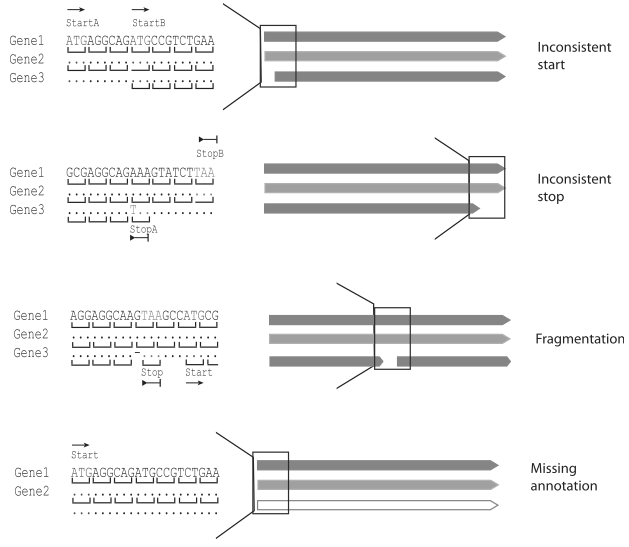
\includegraphics[width=0.66\textwidth]{figures/Introduction/thesis_12}
	\caption{\label{fig:mugsy}\textbf{Incorrect gene annotations}\\
			 Examples of incorrect gene calling that can be corrected thanks to comparative genomics (from \cite{samuel12improving})}
\end{figure}

\subsubsection{Open and closed pangenomes}
\begin{figure}[!tb]
	\center
    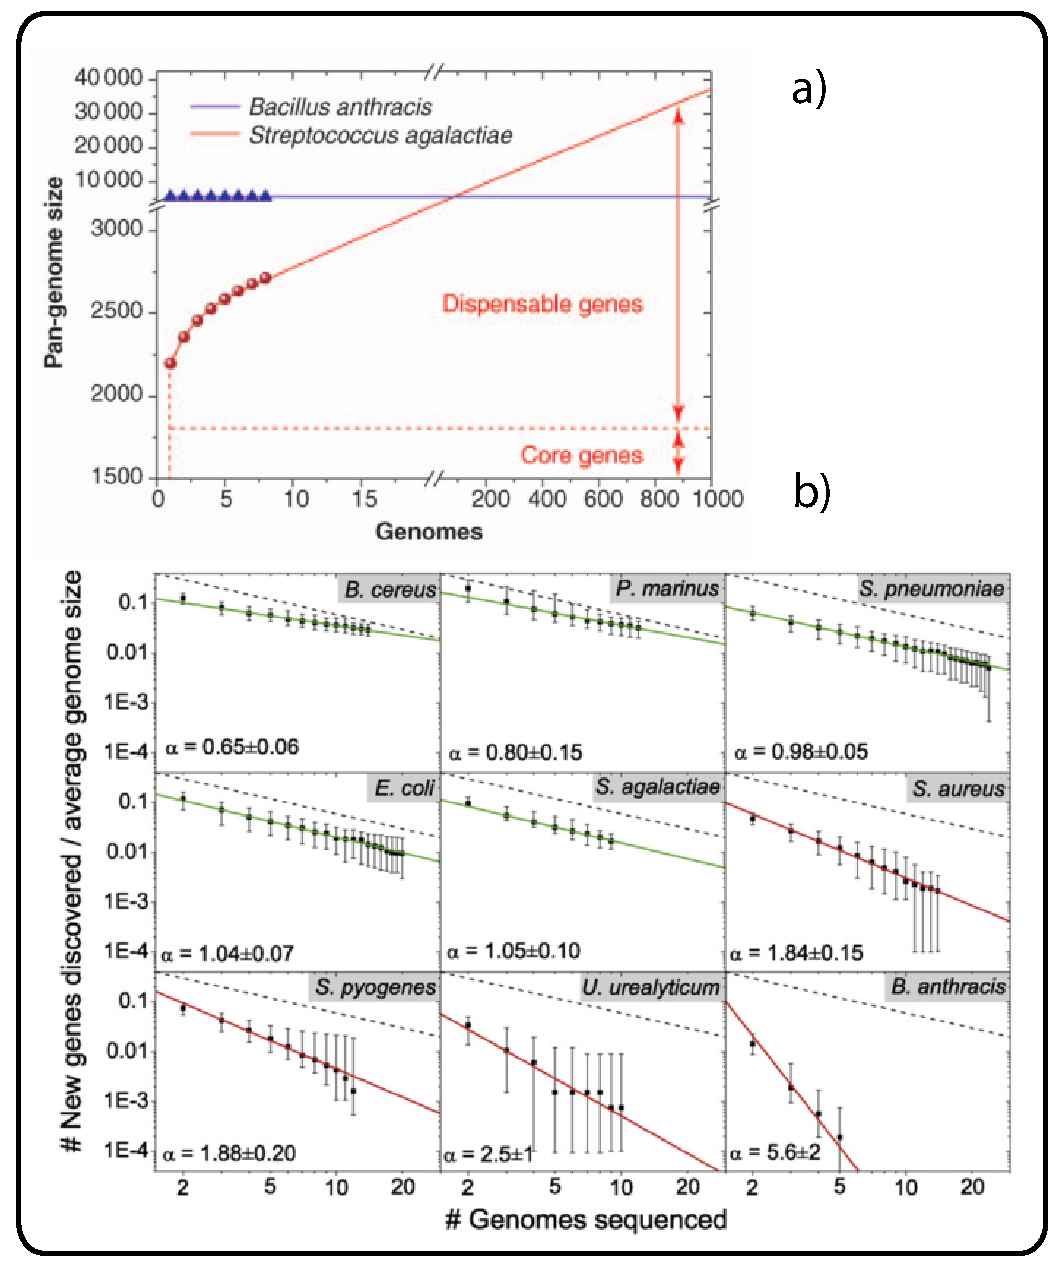
\includegraphics[width=0.8\textwidth]{figures/Introduction/thesis_13}
	\caption{\label{fig:openclosed}\textbf{Open and closed pangenomes}\\
			a) Comparison of the pangenome rarefaction curve between open (\textit{S. agalactiae}) and closed (\textit{B. anthracis}) pangenomes (from \cite{medini2005microbial})\\
			b) Comparison of the new genes discovery rate between open (red lines) and closed (green lines) pangenomes (from \cite{tettelin2008comparative})}
\end{figure}

Another interesting property of the bacterial pangenome is the possibility to infer the lifestyle and the genome evolution of a species solely on the basis of the pangenome rarefaction curve. When the term pangenome was defined, two distinct tendencies in pangenome dynamics were noted: for some genomes many new genes were found for each new genome added to the pangenome, while for some others a significantly smaller amount of new genes were added for each new genome \cite{medini2005microbial} (Figure \ref{fig:openclosed}a). The assumption is that genomes with an evergrowing pangenome probably belong to many and different environments, thus needing a larger gene set to be able to cope with the various nutrients and stress conditions; on the other hand, pangenomes with a relatively low rate of new genes for each genome are probably those that experience a low habitat variability and therefore exhibit a stable genome, like pathogens and obligate symbionts. This observation has been further refined with other genomes, leading to the classification in open and closed pangenomes, described by the fit to the Heaps' law (Equation \ref{eq:heap}): when the $\alpha$ parameter, defined by the fit of the heaps' law to the pangenome rarefaction curve, is $\leq$ 1 the pangenome is described as open, while with $\alpha >$ 1 the pangenome is described as closed. Indeed the species that are found to have a closed pangenomes belong to pathogens and obligate symbionts, like \textit{B. anthracis}, \textit{S. aureus} or \textit{B. aphidicola}, while free-living species like \textit{B. cereus}, \textit{E. coli} or \textit{S. meliloti} are found to have an open pangenome \cite{tettelin2008comparative} (Figure \ref{fig:openclosed}b).

\begin{equation}
\label{eq:heap}
n \sim N^{-\alpha}
\end{equation}

% Here genomic fluidity

\newpage
\section{A tale of two cities: plant-bacteria interaction}
\label{atale2cities}
The bacterial kingdom it's not important just on its own, but also when considering its impact on higher organisms, such as animals, plants and fungi; in recent years, the awareness on the importance of such interactions have grown, with many long-term projects being funded: a notable example is the human microbiome project, aimed at the understanding of the role of the bacterial communities inhabiting the human body in health and physiology \cite{turnbaugh2007human}.

The interaction that is more relevant for this thesis is the plant-bacteria interaction, which indeed is complex and involves a vast range of organisms, strategies and impacts on plants; most importantly, this interactions have been proven to have serious impacts on agriculture, in both economic and environmental terms. These bacteria are often grouped together under the definition of \textit{plant associated bacteria}, but there are many different kinds of plant-bacteria interactions, depending on the occupied niche and on the role in that this bacteria play in the interaction.

\textbf{Occupied plant niche}:
\begin{itemize}
\item \textbf{Endophytes:} those bacteria that colonize the internal tissue of the plant showing no external sign of infection or negative effect on their host \cite{holliday2001dictionary}\cite{schulz2006microbial}; they are further classified as obligate or facultative endophytes. Obligate endophytes are dependent on the plant for their growth and survival, thus being transmitted only through seeds or vectors, while facultative endophytes can also grow in other environments, like the rhizosphere \cite{ryan2007bacterial} (Figure \ref{fig:plantendophytes}).
\item \textbf{Rhizospheric bacteria:} those bacteria inhabiting the plant roots surface and the immediate surroundings where plant essudates are released and stimulate bacterial growth \cite{haas2005biological}; a soil region known as \textit{rhizosphere}, where bacteria play a role in providing nitrogen and phosphorous to the plant, in the protection from parasites and pathogens and in the maintenance of soil structure \cite{singh2004unravelling}.
\item \textbf{Phyllospheric bacteria:} those bacteria inhabiting the surfaces of the plant aerial tissues (also defined as \textit{above ground} tissues), especially on the leaves; these bacteria are also called \textit{epiphytes} \cite{lindow2003microbiology}, and they have a great influence on plant fitness and productivity \cite{whipps2008phyllosphere}.
\end{itemize}

\begin{figure}[!t]
	\center
    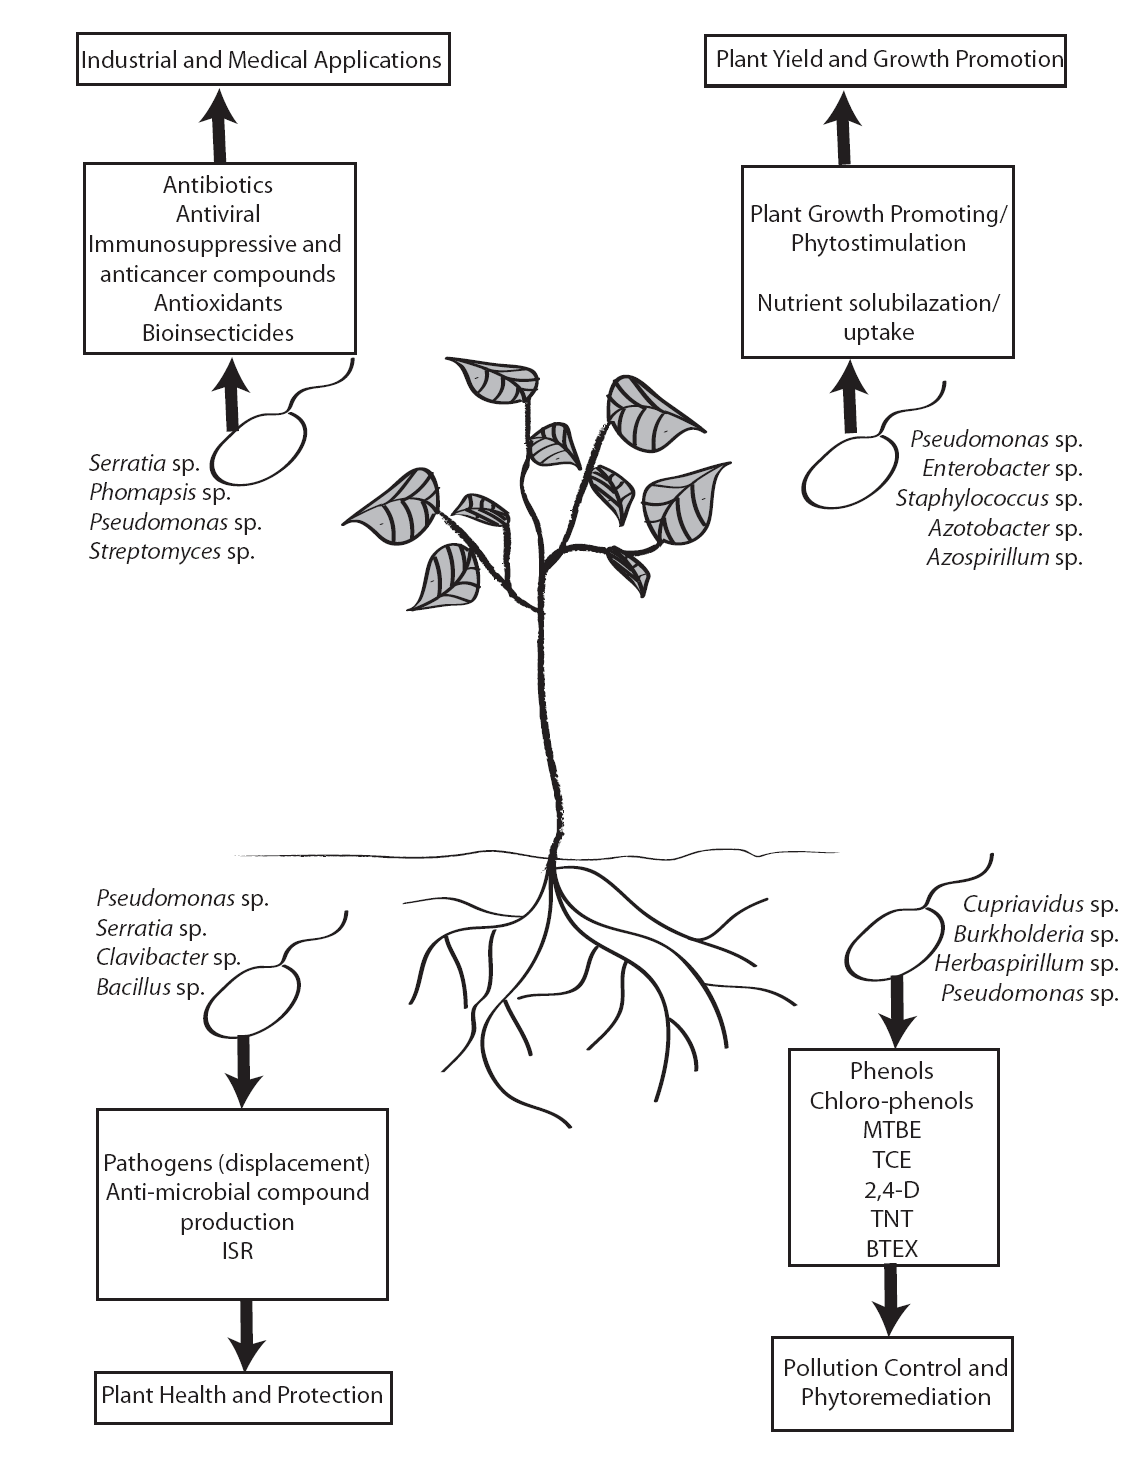
\includegraphics[width=0.7\textwidth]{figures/Introduction/thesis_14}
	\caption{\label{fig:plantendophytes}\textbf{Main players and effects of plant endophytes}\\
			The main species involved in the endophytic interaction and their effect on plant are reported (from \cite{mengoni2011bacterial}, adapted from \cite{ryan2007bacterial})}
\end{figure}

Some bacteria are indeed capable to occupy more than one of this niches, the most notable example being the facultative endophytes, which often inhabit the rhizosphere, later invading plant tissue from cracks in lateral roots or in roots elongation and differentiation zones, probably thanks to the production of cellulolytic and pectinolytic enzymes; the plant is then quickly colonized, with bacterial cells found in the aerial  tissues after one day \cite{rosenblueth2006bacterial}\cite{hallmann1997bacterial}.

All the bacteria that interact with plants can be additionally classified according to their role in the interaction: they can be either commensals, sharing and exchanging nutrients with the plant, pathogens, with deleterious effects on plant health, or symbionts, with a mutualistic interaction.

\begin{figure}[!t]
	\center
    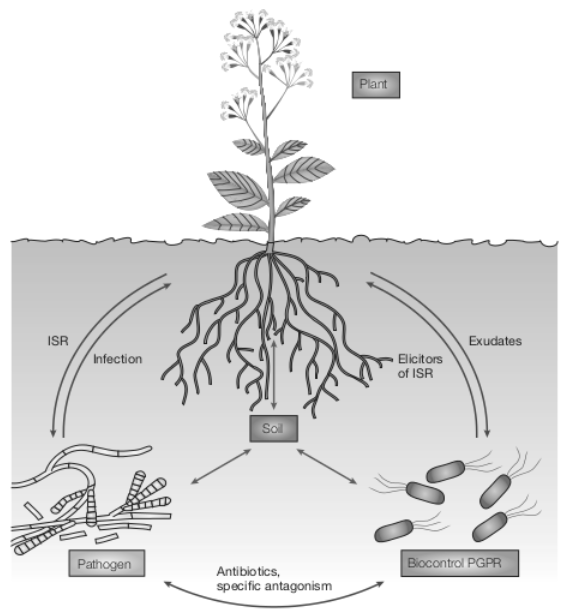
\includegraphics[width=0.7\textwidth]{figures/Introduction/thesis_15}
	\caption{\label{fig:plantprotection}\textbf{Interactions between biocontrol plant growth-promoting rhizobacteria, plants, pathogens and soil}\\
			From \cite{haas2005biological}}
\end{figure}

A particular class of rhizospheric bacteria interacting with plants are termed together under the name \textit{plant growth-promoting rhizobacteria} (PGPR), indicating those bacteria that have a positive impact on plant health and growth. Plant growth is promoted either by protection mechanisms than by nutrient supply: in fact, the  effects of PGPR on plants are divided in indirect and direct; indirect effects include antibiotic protection against pathogenic bacteria, reduction of iron available to phytopathogens in the rhizosphere and exclusion of pathogens by competition (Figure \ref{fig:plantprotection}), while direct effects include the provision of bioavailable phosphourus, nitrogen fixation, syderophore production for plant iron uptake, productions of plant hormonoes and the modulation of the induced systemic resistance (ISR) \cite{vessey2003plant}\cite{lucy2004applications}. This functions can be carried on either by endophytes or symbionts: in fact, some bacterial species can exhibit both plant association phenotypes, like the alphaproteobacterium \textit{Sinorhizobium meliloti} \cite{pini2012exploring}.

%All this beneficial effects take a considerable part in the natural and anthropic plant biology

\subsection{Symbiosis and biological nitrogen fixation}
One of the most important phenotypes that influences plant growth and that has a tremendous impact on agriculture it's the \textit{biological nitrogen fixation} (BNF) process; in fact nitrogen, as one of the most important chemical elements in life, is crucial for a successful plant growth. Nitrogen is an abundant chemical element mainly present as N\textsubscript{2} in the atmosphere (10\textsuperscript{15} tons), with 10\textsuperscript{9} tons that enter the nitrogen cycle each year \cite{postgate1982fundamentals}; the transformation of nitrogen into more available chemical forms has many known mechanisms, both biological and not, such as lightning (supplying 10\% of the annual fixed nitrogen \cite{sprent1990nitrogen}), BNF and anthropogenic chemical N\textsubscript{2}-fertilizers. Today 25\% of the total annual fixed nitrogen comes from anthropogenic chemical nitrogen fixation, while about 60\% comes directly from BNF \cite{peoples1995biological}; the use of N\textsubscript{2}-fertilizers however, has many drawbacks: is expensive, relies on fossile fuels, thus contributing to the climate change, and its usage leads to nitrate water contamination and other pollutions concerns. For this reasons, being able to control the BNF process is a key milestone towards a sustainable agriculture \cite{stewart1966nitrogen}, also considering the growing food safety concerns, especially in less developed countries \cite{n2africa}; on the economic side, the adoption of BNF as the main source of nitrogen for agricultural fertilization would greatly reduce the costs, since about 90 millions tons of nitrogen per year are made available through BNF. 

One of the most important sources of BNF is inside the leguminous plants roots, where rhizospheric bacteria establish a symbiotic interaction, providing fixed nitrogen to plants in exchange of nutrients; this interaction happens inside the plant roots, often in specialized organs called \textit{nodules}. Many bacterial species are able to perform BNF inside leguminous plants, belonging to the alpha and beta proteobacteria subclasses \cite{chen2003legume}. One of the most studies bacterial species associated with leguminous plants is the alphaproteobacterium \textit{Sinorhizobium meliloti}, which establishes a symbiotic relationship with the plant \textit{Medicago sativa} (also termed \textit{alfalfa}). Alfalfa is a perennial leguminous plant from the \textit{Fabaceae} family, known for its resistance to drought and extreme temperatures, but mainly for its high productivity, its nutrients content and its role in soil quality improvement; it's the most cultivated legume in the world, being used as forage, as crop for bioenergy and for the recovery of degraded or marginal lands \cite{vance2001application}\cite{ane2007recent}\cite{bouton1996new}\cite{comisalfalfa}; recently, also the biofuels industry has conducted pilot studies for the utilization of this plant as a source of energy, through the gasification process, using the resulting ashes as fertilizers \cite{mozaffari2000corn}\cite{mccaslin2007future}. The overall world alfalfa production was 436 million tons in 2006, with the United States as the lead producer and Argentina, Australia and South Africa as the other main producers \cite{alfalfa} (Figure \ref{fig:alfalfa}). Thanks to the symbiosis with rhizobial species, alfalfa has an important role in the management of agricoltural lands fertility, and in particular in keeping the bioavailable nitrogen available to other coltures, thus reducing land depletion and the use of chemical fertilizers.

\begin{figure}[!tb]
	\center
    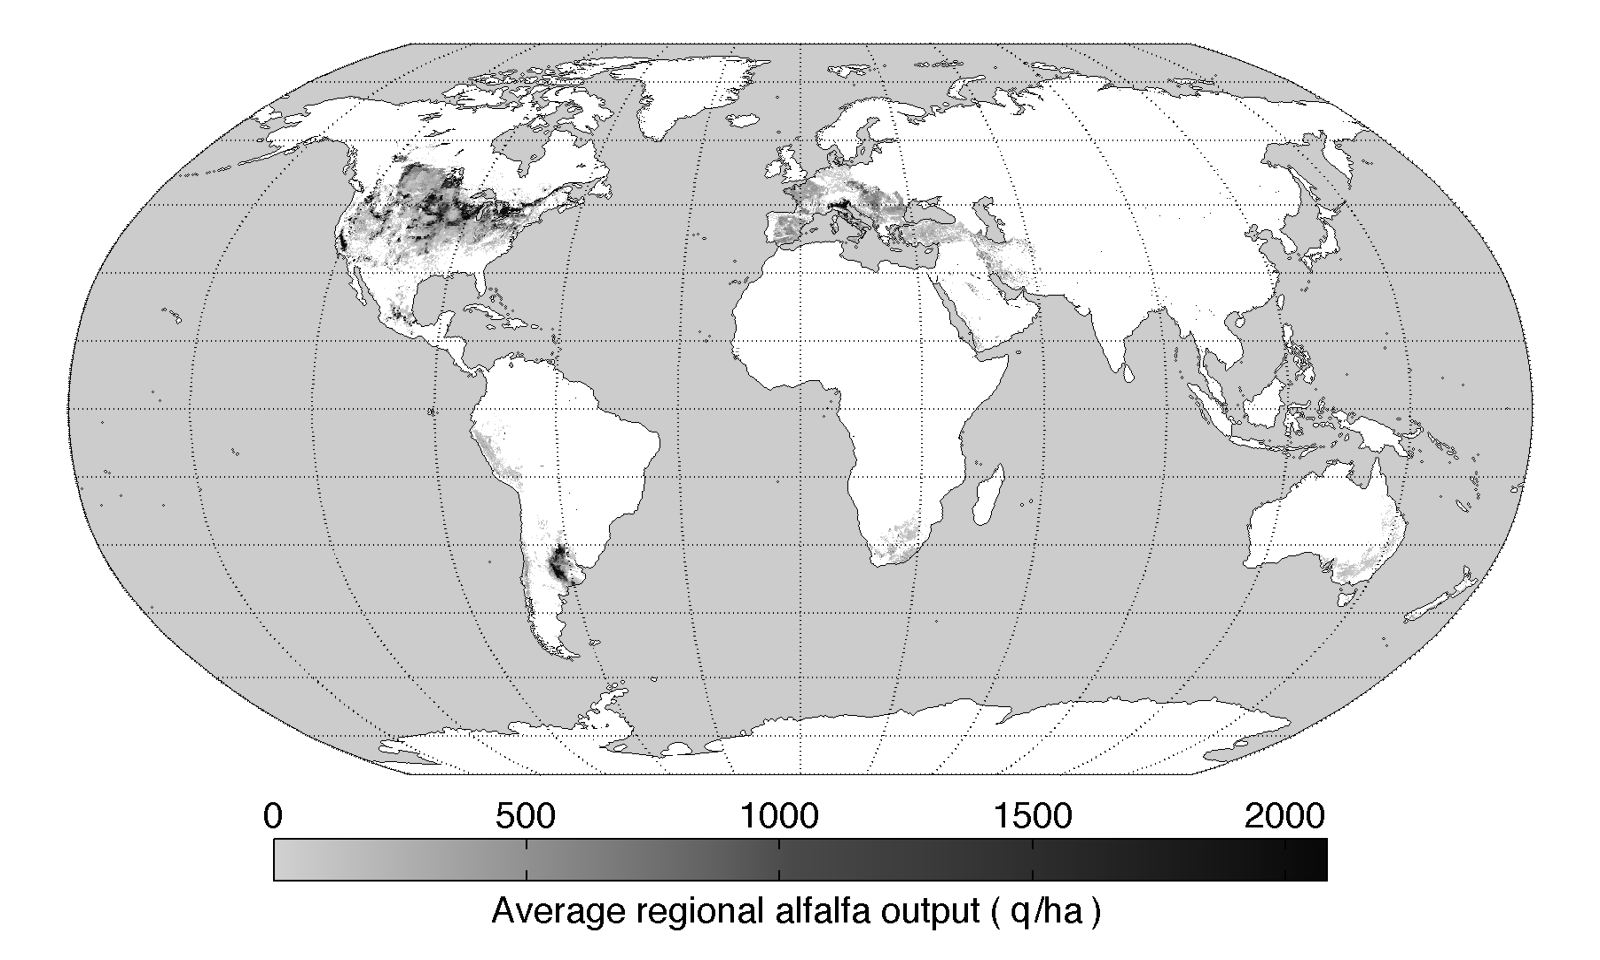
\includegraphics[width=1\textwidth]{figures/Introduction/thesis_16}
	\caption{\label{fig:alfalfa}\textbf{World alfalfa production}\\
			From \cite{alfalfa}}
\end{figure}

The symbiosis between \textit{M. sativa} and \textit{S. meliloti}, like the other known association between leguminous plants and rhizobial species, is a multi-step process involving many exchanges of signals between the plant and the bacteria, and a tight control from the plant on the rhizobial colonization and the N\textsubscript{2}-fixing process \cite{jones2007rhizobial}.

\begin{figure}[!h]
	\center
    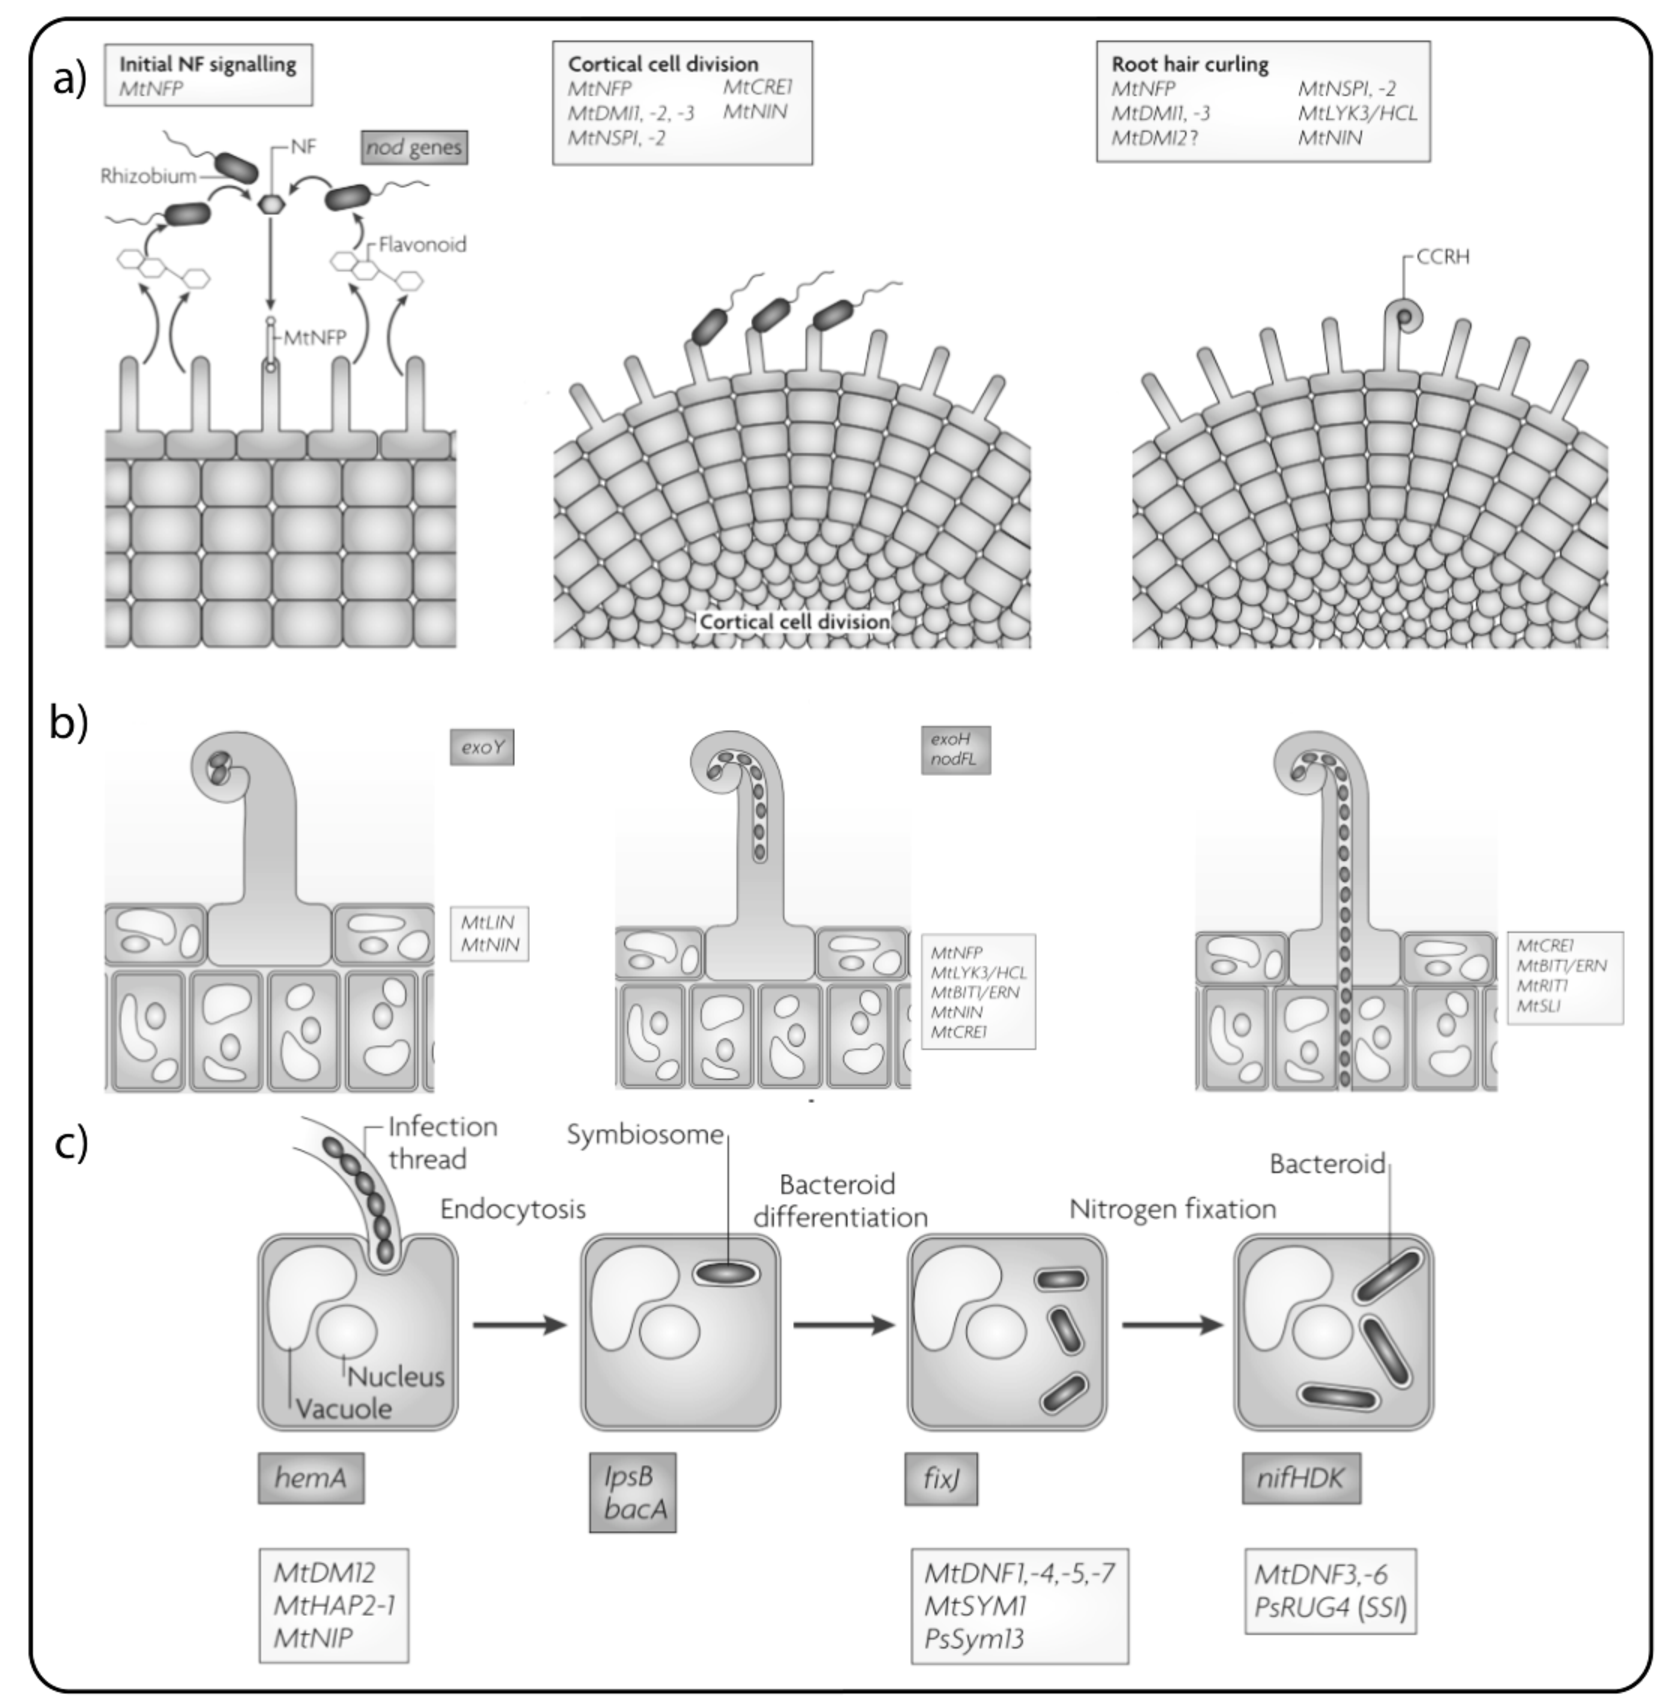
\includegraphics[width=1\textwidth]{figures/Introduction/thesis_17}
	\caption{\label{fig:symbiosis}\textbf{Details on the physiology and genetics of the \textit{S. meliloti} - \textit{M. sativa} symbiosis}\\
			a) Plant - bacteria recognition and adhesion\\
			b) Invasion and infection thread formation\\
			c) Bacteroid differentiation and nitrogen fixation\\
			Adapted from \cite{jones2007rhizobial}}
\end{figure}

%\subsubsection{Agricultural, economic and social impact of BNF}
%Big impact!
%\subsection{The role of the microbial community in the rhizosphere}
%A big role my friend!
%\subsection{Endophytes vs. symbionts}
%A big match!
\subsubsection{Host recognition, invasion and nodule formation}
The first step in the establishment of the symbiosis is the recognition between the plant and the bacterial cells in the rhizosphere: rhizobia sense the root exudates and move chemotaxically towards the roots surface \cite{barbour1991chemotaxis}\cite{caetano1992growth}; in particular, the plant signals recognized by the rhizobia are flavonoids, which are aromatic compounds with a 15 carbon skeleton, produced by the secondary metabolism of the plant. The flavonoids penetrate inside the rhizobial cells, where they are recognized by NodD, the master regulator of the \textit{nod} genes (Table \ref{tab:bnfgenes}), which lead to the production of the so-called \textit{nod factor}, a lipochito-oligosaccharide that is released from the rhizobia and that is recognized by the plant root, and stimulates the production of root hairs that will favour the invasion by the rhizobial cells \cite{shaw2006perception} (Figure \ref{fig:symbiosis}a). The chemical composition of the nod factor is highly specific, precisely determining the so-called host range of the rhizobial species, that are the plant species that recognize that particular nod factor and allow the invasion \cite{kondorosi1984physical}.

\begin{table}
    \begin{tabularx}{\textwidth}{|p{4cm}|p{8.2cm}|}
        \hline
        Gene group              & Function                                                                         \\ \hline
        Common \textit{nod} genes        & Synthesis of the general structure of the nod factor                             \\ 
        Host-specific \textit{nod} genes & Generally not conserved across rhizobial species, determine the host specificity \\ 
        \textit{nif} genes               & Synthesis, regulation and operation of the nitrogen fixation process             \\ 
        \textit{fix} genes               & Regulation of the nitrogen fixation process inside the nodule environment        \\
        \hline
    \end{tabularx}
	\caption{\label{tab:bnfgenes}\textbf{Main genes involved in the establishment of the rhizobia - leguminous plants symbiosis}}
\end{table}

Once that the rhizobial cells adhere to the root hair, thanks to the surface lectins produced by the plant, the local production of nod factor induce a local growth of the root hair, causing a curled development that traps the rhizobial cells on the root hair tip \cite{diaz1986correlation}. An hydrolysis on the plant cells wall leads then to the formation of the so-called \textit{infection thread}, a tubular growth of the rhizobial cells along the root hair (Figure \ref{fig:symbiosis}b).

When the infection thread reaches the base of the root hair, the rhizobial cells are internalized by the bark cells and are included by endocytosis in vescicles termed \textit{symbiosomes}, where they undergo a series of physiological changes to a form termed \textit{bacteroid} \cite{brewin2004plant}, while the plant root cells are growing, leading to the formation of the nodule, an oval organ attacched to the root. Depending on the shape and internal physiology of the nodule, they can be divided in two groups, \textit{determined} and \textit{indetermined}, with the latter being typical to the \textit{Sinorhizobium} - \textit{Medicago} symbiosis (Figure \ref{fig:symbiosis}c).

\begin{itemize}
\item \textbf{Determined nodules:} this nodules are typical of tropical and subtropical legumes, are characterized by a globolose shape, the absence of a meristematic activity; bacteroid found in this nodules are comparable to free living cells in terms of DNA content, cell shape and size and viability \cite{brewin1991development}\cite{franssen1992developmental}\cite{mergaert2006eukaryotic}.
\item \textbf{Indetermined nodules:} this nodules, typical of temperate legumes, have a more elongated shape (caused by a persistent meristematic activity) and with the internal rhizobial cells showing a distinct degree in differentiation in bacteroids (with five distinct differentiation steps) in the various zones of the nodule (four distinct zones) \cite{patriarca2002key}\cite{pawlowski1996rhizobial}\cite{vasse1990correlation}.
\end{itemize}

The bacteroids found in indeterminate nodules are bigger in size, more elongated and with an increased DNA content, with multiple nucleoids; the cells viability is highly reduced when rhizobial cells are in this state, most probably because of serious impairs in the cell cycle \cite{mergaert2006eukaryotic}.

\subsubsection{Nitrogen fixation}
The process of BNF is mediated through the enzyme nitrogenase, which converts the inert atmospheric nitrogen (N\textsubscript{2}) to the accessible form of ammonia (NH\textsubscript{3}) \cite{peters2006exploring}; this enzyme is present in prokaryotes (the groups \textit{Rhizobia}, \textit{Cyanobacteria}, \textit{Azobacteria}, the genus \textit{Frankia}) and some \textit{Archaea} \cite{raymond2004natural}. In the \textit{Sinorhizobium} - \textit{Medicago} symbiosis, the nitrogen fixation takes place inside the nodules symbiosomes by the differentiated bacteroids, which exhibit a significant downregulation of many metabolic functions, together with an upregulation of the genes related to nitrogenase activity \cite{barnett2006global}; this particular enzymatic  activity needs a considerable amount of energy, with 16 ATP molecules needed to fix a single molecule of atmospheric nitrogen \cite{poole2000carbon}, energy that is provided by the plant, in the form of photosynthesis products in return of the fixed ammonia \cite{lodwig2003metabolism}. Another key factor for an efficient BNF is the O\textsubscript{2} concentration, which inhibits the nitrogenase activity, but it is also needed for cellular respiration: the modulation of the oxygen concentration inside the nodule is therefore critical for the overall BNF process; this regulation is performed thanks to the leghaemoglobin, which is constituted by an heme produced by the rhizobial cells and a globinic part provided by the plant \cite{o1987bacterial}. The presence of the leghemoglobin confers the typical light-red color of the nodules in which active nitrogen fixation is carried on (Figure \ref{fig:nodules}).

\begin{figure}[!tb]
	\center
    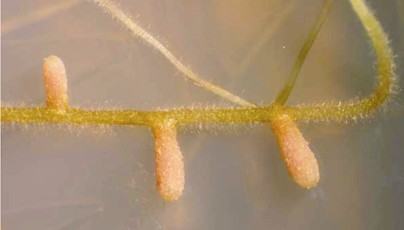
\includegraphics[width=0.66\textwidth]{figures/Introduction/thesis_18}
	\caption{\label{fig:nodules}\textbf{Nodules with active BNF}\\
			Indeterminate nodules exhibiting the typical light-red color of active nitrogen fixation, from a \textit{Sinorhizobium} - \textit{Medicago} nodulation experiment}
\end{figure}

\subsubsection{Genomics of symbiosis in \textit{S. meliloti}}
\label{sec:genomicsmeliloti}
Given the agricultural, economical and environmental importance of the \textit{Sinorhizobium} - \textit{Medicago} symbiosis, a considerable effort has been put towards the understanding of the genetic basis of this symbiosis: thanks to the technological advances in bacterial genomics, the first complete genomic sequence of a \textit{Sinorhizobium meliloti} strain was obtained in 2001 \cite{galibert2001composite}. The genome of this species is considerably bigger than many other bacteria, with 6.7 Mb (E. coli has a genome of about 4.5 Mb) and a peculiar multipartite structure, harboring a chromosome (3.65 Mb) and two megaplasmids termed pSymA (1.35 Mb) and pSymB (1.68 Mb); the presence of housekeeping functions on the latter megaplasmid has lead to its recent redefinition as a \textit{chromid}, that are megaplasmids with comparable GC content to the main chromosome and harboring essential genes \cite{harrison2010introducing}. The relative large genome of S. meliloti, together with the high number of paralogs and duplicated regions is consistent with the life-style of this species, since it needs to perform an efficient nitrogen fixation to avoid plant sanctions \cite{denison2004most}, and because of the competition inside the rhizosphere and in soil. An interesting genetical and evolutionary feature of this multipartite genome it's the different functional signature of each replicon, with most of the house-keeping genes present in the chromosome, most of the small molecules transporters belonging to pSymB and the vast majority of the genes needed for symbiosis, (including various duplicated copies) and nitrogen metabolism (\textit{nos}, \textit{nor}, and \textit{nap}) belonging to pSymA, whose codon usage and GC content supports the thesis of its origin by horizontal gene transfer events. There are also evidences of a spacial localization of some key symbiotic genes located on the pSymA replicon, with a particular focus on genes expressed in the bacteroid form and in microoxic conditions \cite{becker2004global} (Figure \ref{fig:spacial}), a feature that supports the thesis of an HGT origin of the symbiotic cluster. 

\begin{figure}[!tb]
	\center
    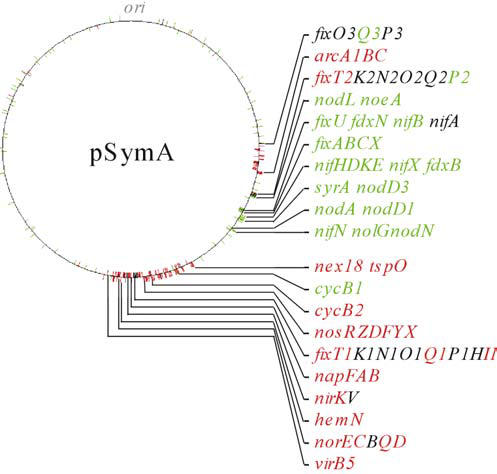
\includegraphics[width=0.6\textwidth]{figures/Introduction/thesis_19}
	\caption{\label{fig:spacial}\textbf{Spacial organization of key symbiotic genes on the pSymA megaplasmid}\\
			Position of genes induced in microoxic conditions (red), of genes induced in bacteroids (green) and in both conditions (black) (from \cite{becker2004global})}
\end{figure}

\subsubsection{Natural variability of \textit{S. meliloti}}
The genomic analysis on the \textit{Sinorhizobium meliloti} Rm1021 strain has been an important landmark in the understanding of the symbiotic process; however there are still some aspects of the \textit{Sinorhizobium} - \textit{Medicago} symbiosis that need to be studied, in order to optimize this process and extend it to a more rational use for the growing need of the modern world. A key point that needs to be addressed is the extent and the genetic origin of the natural diversity in the various aspects of the plant growth promotion phenotype, including the increase in plant growth, the resistance to specific environmental stresses like high salt concentration and host specificity; understanding the evolutionary dynamics of the composite genome is also an interesting issue, since it may shed some light on the origin of the symbiotic genes and to what extent they are conserved inside rhizobia. The final goal of such studies would be the definition of a series of genetic elements that are correlated with desirable plant growth promoting phenotypes, that can be then used with genetic engineering approaches towards the design of new strains of \textit{Sinorhizobium meliloti}. Some studies using CGH arrays have already established that there is indeed a certain degree of genetic diversity between different strains of \textit{S. meliloti}, exhibiting differences in the plant growth promoting ability \cite{giuntini2005large}: about 5\% of the genes of the Rm1021 strain showed signs of genetic variability in four natural strains, with the majority of this mutations occurring on the megaplasmid pSymA, suggesting an important role of this replicon in explaining the observed phenotypic variability.

%%-----------
%% Backmatter
%%-----------
\backmatter
\chaptermark{Bibliography}
\renewcommand{\sectionmark}[1]{\markright{#1}}
\bibliographystyle{unsrt}                           %Use alpha codes for references
\sectionmark{Bibliography}
\addcontentsline{toc}{chapter}{Bibliography}        %Force addition of Bibliography to TOC    
\bibliography{References}                                  %Introduction

\mainmatter
\part{Results}
%%%%%%%%%%%%%%%%%%%%%%%%%%%%%%%%%%%%%%%%%%%%%%
\logvartrue
\chapter{New tools for new data: comparative genomics software}
%%%%%%%%%%%%%%%%%%%%%%%%%%%%%%%%%%%%%%%%%%%%%%

The quick development of the next generation sequencing technologies have posed serious challenges for the analysis of the high quantity of data produced: new softwares being able to catch up with the technological progress are therefore needed, not only for raw analysis purposes, but also for the constant need to draw a comprehensive picture of the cellular processes and their genetic and molecular components. The first part of this thesis will therefore be focused on the development of two tools dedicated to the analysis of highthroughput technologies data: the objective of these softwares are an easier analysis on these complex new data and, most importantly, the combination of different data sources in the construction of a detailed view on cell biology. A particular focus has been put towards the so-called \textit{usability}, meaning that the developed software should be easy to use and well documented, features that are usually not implemented in most of the now available bioinformatic programs \cite{corpas2012not}. The problems addressed by the two softwares described in this section are the ability to gain structural insights from draft genomes and the ability to provide genetic explanations to phenotypic differences; examples of the utilization of these softwares can be found in Appendix \ref{sec:appendix1}.

\section{The challenges of the \textit{omics} technologies}
\subsection{Improvement of draft genomes using reference genomes}
\begin{figure}[!tb]
	\center
    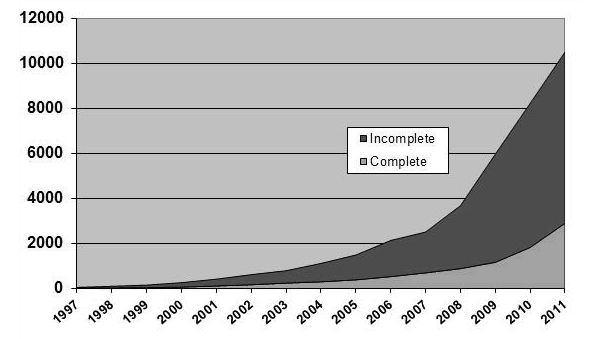
\includegraphics[width=0.7\textwidth]{figures/2/thesis_20}
	\caption{\label{fig:golddraft}\textbf{Sequencing status of the genomic projects}\\
			Number of genomic projects in draft or completed form registered in the GOLD database, October 2011 (from \cite{gold})}
\end{figure}

The recent increase in the number of bacterial genomes available has not seen an equal increase in the number of \textit{finished} genomes, meaning that often the sequences will remain in the so-called \textit{draft} form, as a series of contigs; in fact, most of the recent new genomic projects are submitted in their draft form and are most probably not going to be closed at all \ref{fig:golddraft}. A genome in draft form it's still usefull for genomic and comparative genomics studies, since most of the ORFs can still be predicted with sufficient accuracy (and some gene annotators softwares can handle the ORFs prediction on draft genomes \cite{hyatt2010prodigal}); what is missing it's the possibility to perform structural genomics analysis or to precisely determine the number of replicons and their size. This considerations lead to the need for a new software that would have speeded up the genome finishing phase, with also the ability to gain structural insights from closely related genomes for all those bacterial genomes that would have remained permanently in the draft form.

\subsection{The missing link between genomics and phenomics}
Another key objective in modern biology is the ability to understand the genetic and molecular basis of the phenotypic variability observed in the bacterial kingdom, even inside the same taxonomical unit, such as genera or species. Old molecular techniques allowed the analysis only on small subsets of genotypes and phenotypes for each iteration; however, the advances in the genomic science allow biologists to define the entire genotype of a defined species, while new recent developments in the young field of highthroughput phenomics now allow to obtain a detailed phenotypic picture with relatively limited effort (see for instance the Phenotype Microarray technology \cite{biologPM}). Even though the ability to obtain complete genotypes and sufficiently detailed phenotypes is now easier, to date no tools are available for a comprehensive analysis on the combination of both datasets; indeed some frameworks are already able to provide a skeleton for such studies, like the KEGG metabolic networks, in which both the enzymes mapped in a genome and a series of compunds can be used and linked together \cite{ogata1999kegg}, and may be used to provide clues on the genetic explanations of the phenotypic variability.

\newpage
\section{CONTIGuator: a bacterial genome finishing tool for structural insights on draft genomes}
As discussed in the introduction, one of the main drawbacks of the recent sequencing technologies revolution is the fact that the finishing step is still time consuming and poorly automated, having to rely on an often huge number of PCR reactions to close the remaining gaps between the obtained contigs. Having a closed genome is important to draw a precise functional picture of the strain, because all the ORFs (as well as other functional elements) can be predicted; most importantly, a closed genome is needed for structural genomics analysis, as well for comparative structural genomics. However, since the rate (and cost) of genome finishing it\'s not expected to catch up with the rate of genome sequencing, there is the strong need for computational approaches that allow both an easier way to design the PCR reactions for gap closure and the possibility to predict the functional features of the genome using only the draft sequence. An additional degree of complexity is given by the fact that many bacterial genomes are constituted by more than one replicon, a feature that most of the available programs do not address, leading to less accurate maps for this particular kind of genomes. 
The CONTIGuator software was designed and developed to address these issues: the contigs that constitute the draft genome are mapped to closely related reference genomes, in order to infer their relative orientation, as well to highlight putative structural features. The output of the program comprise a series of structural maps (viewable through the sanger Artemis Comparison Tool \cite{carver2005act}), and a set of primers, which could help in reducing the number of PCR reactions that are needed to close the gaps between each contig.
The software was compared to existing solution, showing that in many cases there was a substantial gain in the the number of bases mapped to the target genome, as well as an higher number of putatively closed gaps.
\newpage
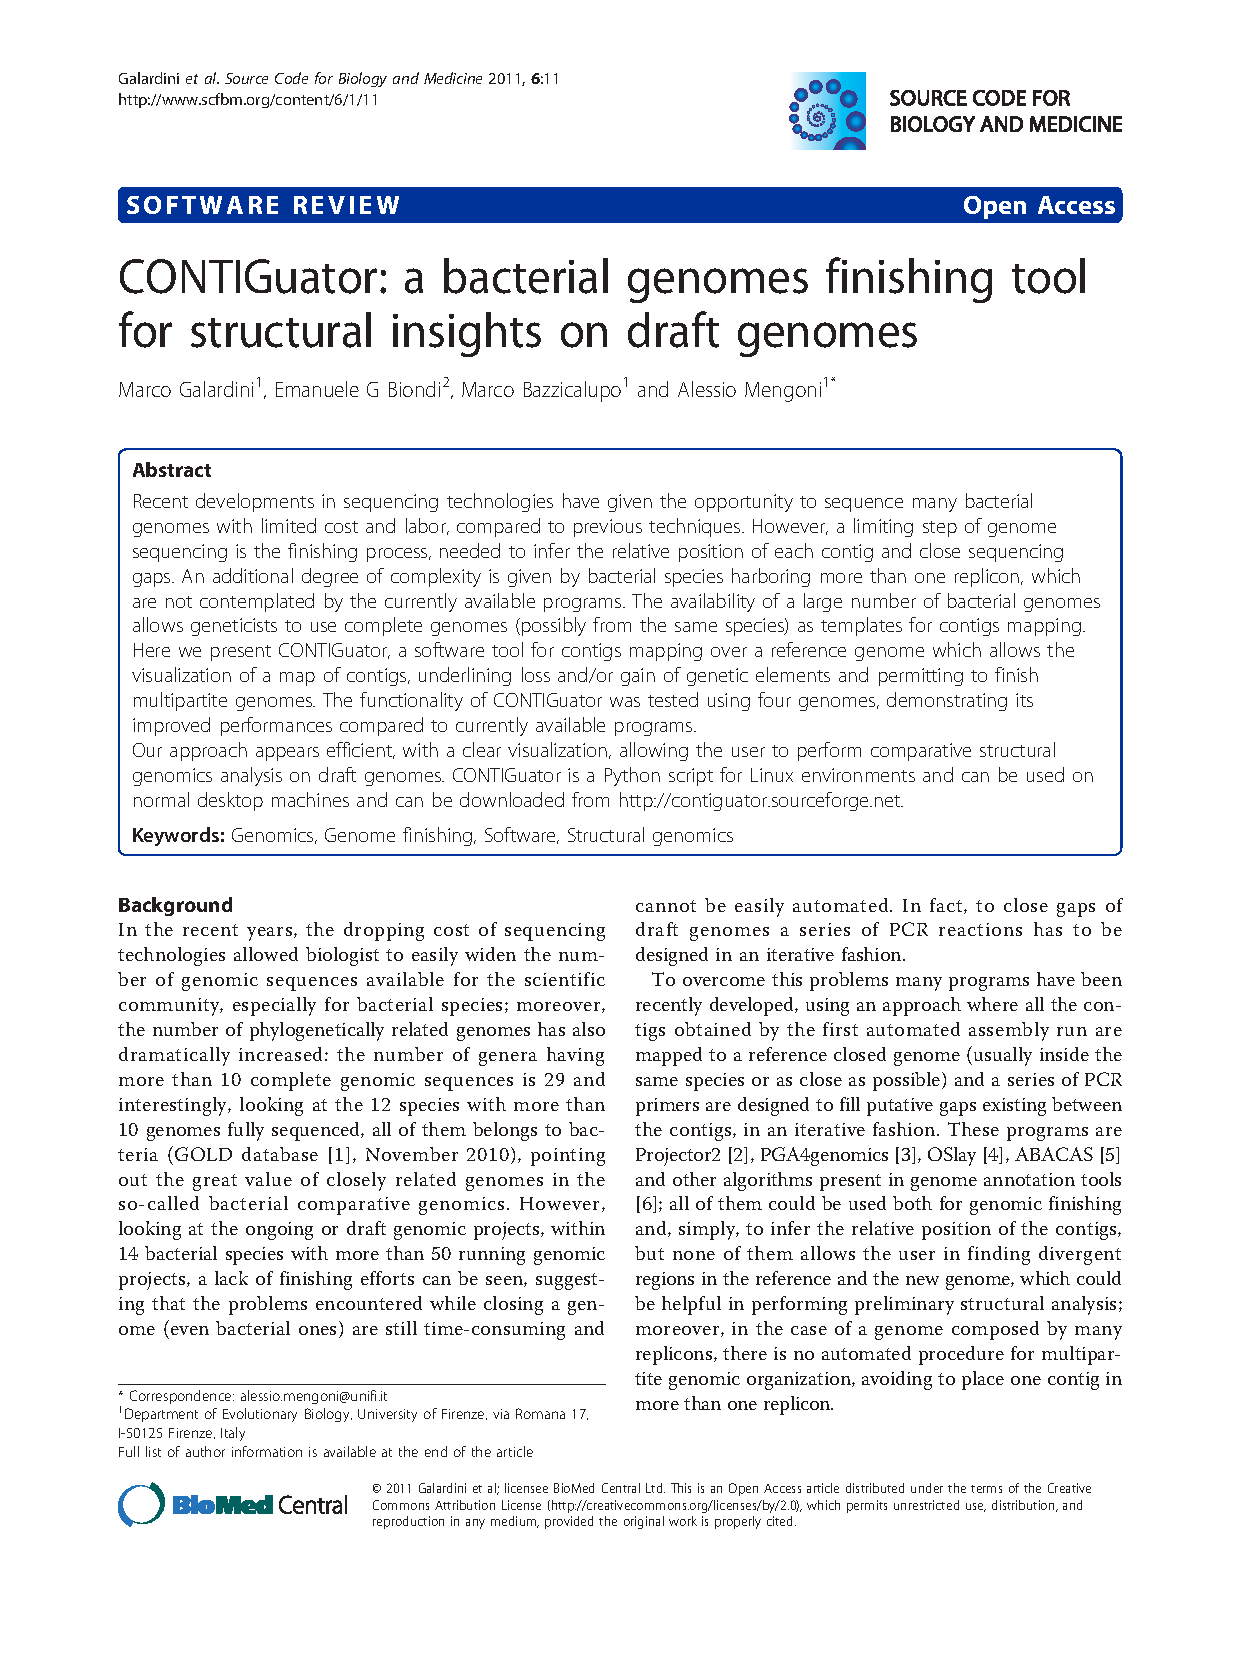
\includepdf[pages=-,offset=10mm 0, scale=0.9]{articles/Galardini2011b.pdf}

\newpage
\subsection{Further developments: version 2 and the CONTIGuator web server}
\begin{figure}[!b]
	\center
    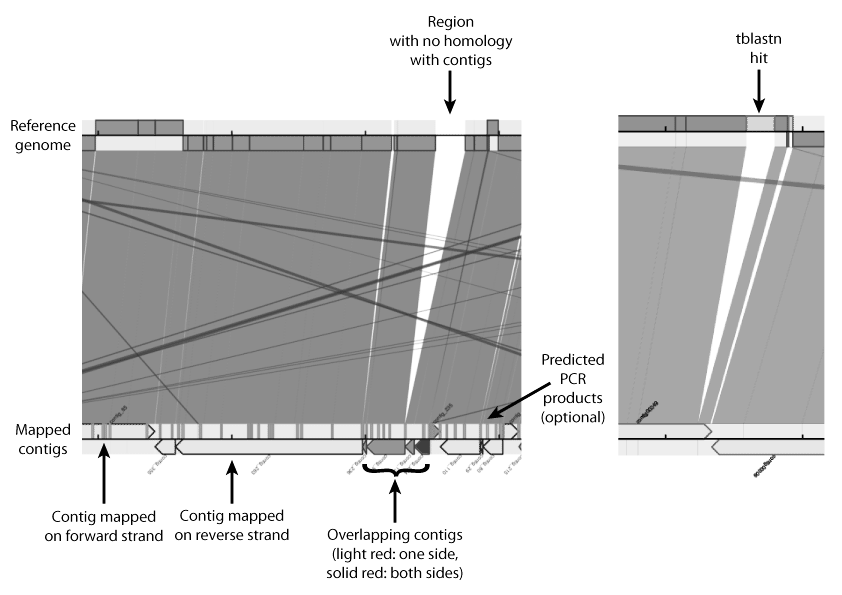
\includegraphics[width=0.9\textwidth]{figures/2/thesis_25}
	\caption{\label{fig:contiguator2}\textbf{CONTIGuator 2 contig maps legend}\\
			from \cite{contiguator}}
\end{figure}

Even though the first version of CONTIGuator was able to provide the needed informations for a faster finishing phase and for a first structural insight, good programming pratices dictate a continuos curation on software features, performances and a prompt bug fixing, together with a continuos enhanchment of the usability and results visualization. The constant help of the scientific community has lead to the second version of CONTIGuator, in which many bugs caused by genomes with peculiar features (like the presence of contigs spanning on the starting point of the reference genome sequence) have been fixed, as well as compatibility with older and newer versions of all the software needed by the program (such as primer3 \cite{rozen2000primer3}, biopython \cite{cock2009biopython} and blast \cite{camacho2009blast+}). The main improvements however, are in the output formats and in the usability features: many new files are produced by the program in order to help a faster analysis on those contigs that have been mapped by the program and those that are not mapped; also the contig maps, that are necessary to gain the structural insights have been improved, with a faster and automated launch of the ACT \cite{carver2005act} program and the generation of static maps in pdf format, thanks to the GenomeDiagram package inside biopython \cite{cock2009biopython}\cite{pritchard2006genomediagram}, which are best suited for exchange and publications (Figure \ref{fig:contiguator2}).

\begin{figure}[!tb]
	\center
    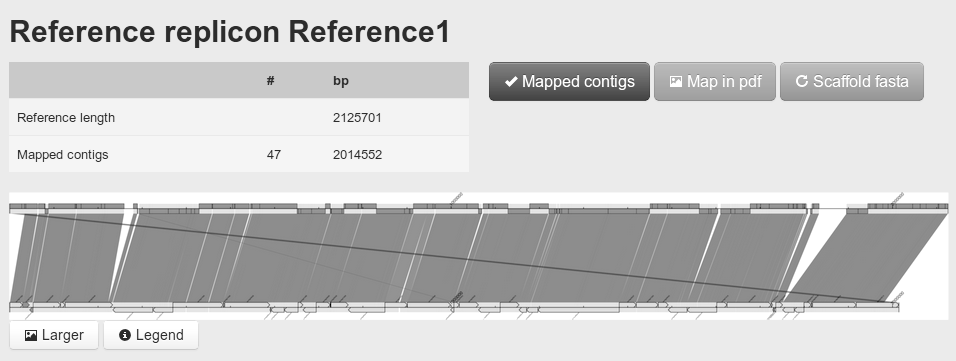
\includegraphics[width=0.9\textwidth]{figures/2/thesis_26}
	\caption{\label{fig:contiguatorweb}\textbf{The CONTIGuator web interface results page}\\
			from \cite{contiguator2}}
\end{figure}

A further step forward in terms of usability has been the development of a web interface to the program, which allows users that are not experts in the field of bioinformatics to use the program and to analyze the results: the software features are the same as the regular command line version, but from the user perspective, there is no need to install any program or to learn any bioinformatic skills (Figure \ref{fig:contiguatorweb}). In fact the number of users that have used the program since September 2012 to December 2012 are more than one hundred. 

\newpage
\section{DuctApe: a tool for analysis and correlation of genomic and high throughput phenotype data}
\label{sec:ductape}
Understanding the functionality of genomes is one of the most important and challenging tasks of today's biology. In particular the linkage between genomes and corresponding phenotypes (i.e. metabolic abilities) is of particular interest in the reconstruction and biotechnological modification of metabolic pathways and also in the study of their evolution. In the last years, the Omnilog\texttrademark Phenotype Microarray (PM) technology has been used to address many specific issues related to the metabolic functionality of microorganisms. However a software which could directly link PM data with the genome(s) of interest, then extracting the information on gene-phenotype correlation is still missing. Fot this purpose DuctApe was developed, a software tool that allows to analyse genome sequences and PM data, finding and visualize any metabolic difference among PM experiments and to correlate them with KEGG pathways and gene presence/absence patterns.

Source code and tutorial are freely available on \href{http://combogenomics.github.com/DuctApe/}{GitHub} (@combogenomics). DuctApe is written in Python and can be installed in UNIX environments\footnote{Authors: \textbf{Marco Galardini}, Alessio Mengoni, Emanuele G. Biondi, Alessandro Florio, Marco Bazzicalupo, Stefano Mocali}.

\subsection{Introduction}
In the recent years the continue development and success of new sequencing instruments, (so-called ”next generation” or ”massively parallel"), have exponentially increased the high-throughput DNA sequencing which is becoming available and affordable even for small labs, which are potentially able to sequence hundreds of bacterial strains per year \cite{metzker2009sequencing}. Actually the reduced time and costs of genomic analysis have already allowed the achievement of over 2100 prokaryotic complete sequences (on October 2012). Although a number of other “omics” techniques have determined a terrific contribution to address fundamental biological questions in microbiology (i.e. transcriptomics, proteomics, metabolomics, metagenomics, etc.) \cite{zhang2010integrating}, the cell phenotype represent the final expression of the genomic information and the result of all the components described by the previously addressed “omics” techniques. Furthermore, most of the genes from genomic sequencing efforts have no ascribed function, and even genes with ascribed functions are based primarily on DNA sequence homology, with little or no direct experimental data \cite{mardis2008impact}. In order to assess a rapid functional and phenotypic profiling under different conditions, a high-throughput approach was developed by BIOLOG Inc. (Heyward, CA): the Phenotype Microarray (PM) technology. PM technology, based on the OmniLog\texttrademark platform, is a system designed for metabolic and antibiotic resistance assays of both bacterial and eukaryotic strains in 96-well PM plates comprising a total of 2400 physiological challenges under temperature-controlled conditions. In each well the physiological reaction can be monitored using cell respiration as a reporter system. Indeed if the cell can catabolize the substrate there will be a flow of electrons from the carbon source to NADH, which determines the reduction of a tetrazolium violet dye and the consequent production of a purple colour (formazan) \cite{bochner2001phenotype}. The colour change is then recorded by an automatic camera every 15 minutes, providing a huge amount of data over the course of several days. These data are directly stored in the computer and can be analyzed by means of OminoLog\texttrademark PM software \cite{biolog2009}. However, managing the data produced in these experiments is not immediate and practical. Some software, which could enhance the tools supplied with the OmniLog\texttrademark instrument have been proposed, such as PhD database \cite{li2005phd}, the RetroSpect\texttrademark software \cite{biolog2008} and PheMaDB \cite{wenling12phemadb}. However such applications are mainly customized databases which have been developed for the management and the storage of phenotypic data obtained from the OminoLog\texttrademark PM software, which displays the PM measurements as 96-wells plate layout and provides few single kinetic parameter values from each curve, without considering the entire curve shapes and kinetics. In fact, as recently highlighted by Vaas and co-workers (2012), the PM respiration kinetics contain additional valuable biological information that go significantly beyond the mere presence/absence measurements and which need to be better exploited. In their work the authors proposed a R-based software solution (package \textit{opmdata}) for exploiting multiple respiration curves from PM data and providing also a detailed statistical estimation of the results. Although the visualization of the PM raw data was significantly improved as compared to the native Omnilog\texttrademark PM software, unfortunately any useful tool for linking the results to putative metabolic pathways is  provided. Nevertheless a tool for comparing and linking genomic and phenomic data is also unavailable. The opmdata package provides four parameters for each growth curve, which is useful for a deeper analysis on single curves; however, such a multidimensional approach doesn't allow a direct way of comparison of entire datasets, or the inclusion of the phenotypic information inside the metabolic network. To better face this challenge and fill this gap we have designed an easy-to-use software system called DuctApe, which links together both the genomic and the phenomic data and suggests genetic explanations of metabolic phenotypes. The software uses the KEGG database as a source of information for metabolic pathways, divided in reactions (that are the proteins in each genome) and compounds; this is where DuctApe comes to help, mapping the genome content and the compounds into the same metabolic maps. It also provides various network statistics to help predict which parts of the metabolic network may be more related to the utilization of a specific compound. Furthermore, several kinds of experimental setups can be analyzed: 

\begin{itemize}
\item single strain experiment,
\item mutational experiments with one reference strain and one or more mutants,
\item pangenomic experiments with more than one organism simultaneously.
\end{itemize}

Several works have been published to assess the link between genomic and PM data \cite{biondi2009metabolic}\cite{viti2009involvement}\cite{peleg2012success} or attempted to improve genome annotation \cite{reed2006towards}, but the managing of data produced in these experiments did not cover all the potential information within the dataset. Here, we tested DuctApe on two PM datasets: the first one from four strains of the symbiotic nitrogen-fixing model bacterium \textit{Sinorhizobium meliloti}, determined on PM 1,2,3,4,5,9 and 10 (\cite{biondi2009metabolic}; the second one comprised the same four strains but their phenotype was determined by using the entire OmniLog\texttrademark system plate set and compared to their previously sequenced genomes \cite{galardini2011exploring}.

\subsection{System and methods}
The tool has been developed as a \textit{“suite”}, which is constituted by three individual modules: 1) DuctGenome (\textit{dgenome}): for genomic data analysis; 2) DuctPhenome (\textit{dphenome}): for PM data analysis; 3) DuctApe (\textit{dape}): for genomics and phenomics linking; the third module is also used to manage to setup the experiment and handle the KEGG data.
 
\subsubsection{DuctGenome (dgenome)}
The first module is used to handle the genomic data from the strains of the experiment, and to return the metabolism reconstruction according to the KEGG database, as a series of pathway maps in which the proteins encoded in the genome are mapped and putatively assigned to a metabolic task. The user can directly provide the list of KEGG identifiers (i.e. the KEGG orthology IDs given by the KAAS automatic annotation server \cite{moriya2007kaas}) or a local KEGG database to which the proteins of each organism will be queried through a Blast-BBH, using the Blast+ software \cite{camacho2009blast+}. Once that a list of KEGG identifiers is available, the metabolic network is reconstructed using the KEGG API (Application Programming Interface). The metabolic map reconstruction will be used by the dape module. If a pangenomic experiment is set, the information on the conserved, accessory and unique metabolisms can be extracted through the detection of all the orthologs (the so-called pangenome); the user can provide the orthologs classification as provided by an external algorithm, like InParanoid \cite{ostlund2010inparanoid} or use the internal parallel Blast-BBH approach \cite{popa2011directed}. The protein sequences are handled by the BioPython package \cite{cock2009biopython}.

\subsubsection{DuctGenome (dphenome)}
\begin{sidewaysfigure}
	\center
    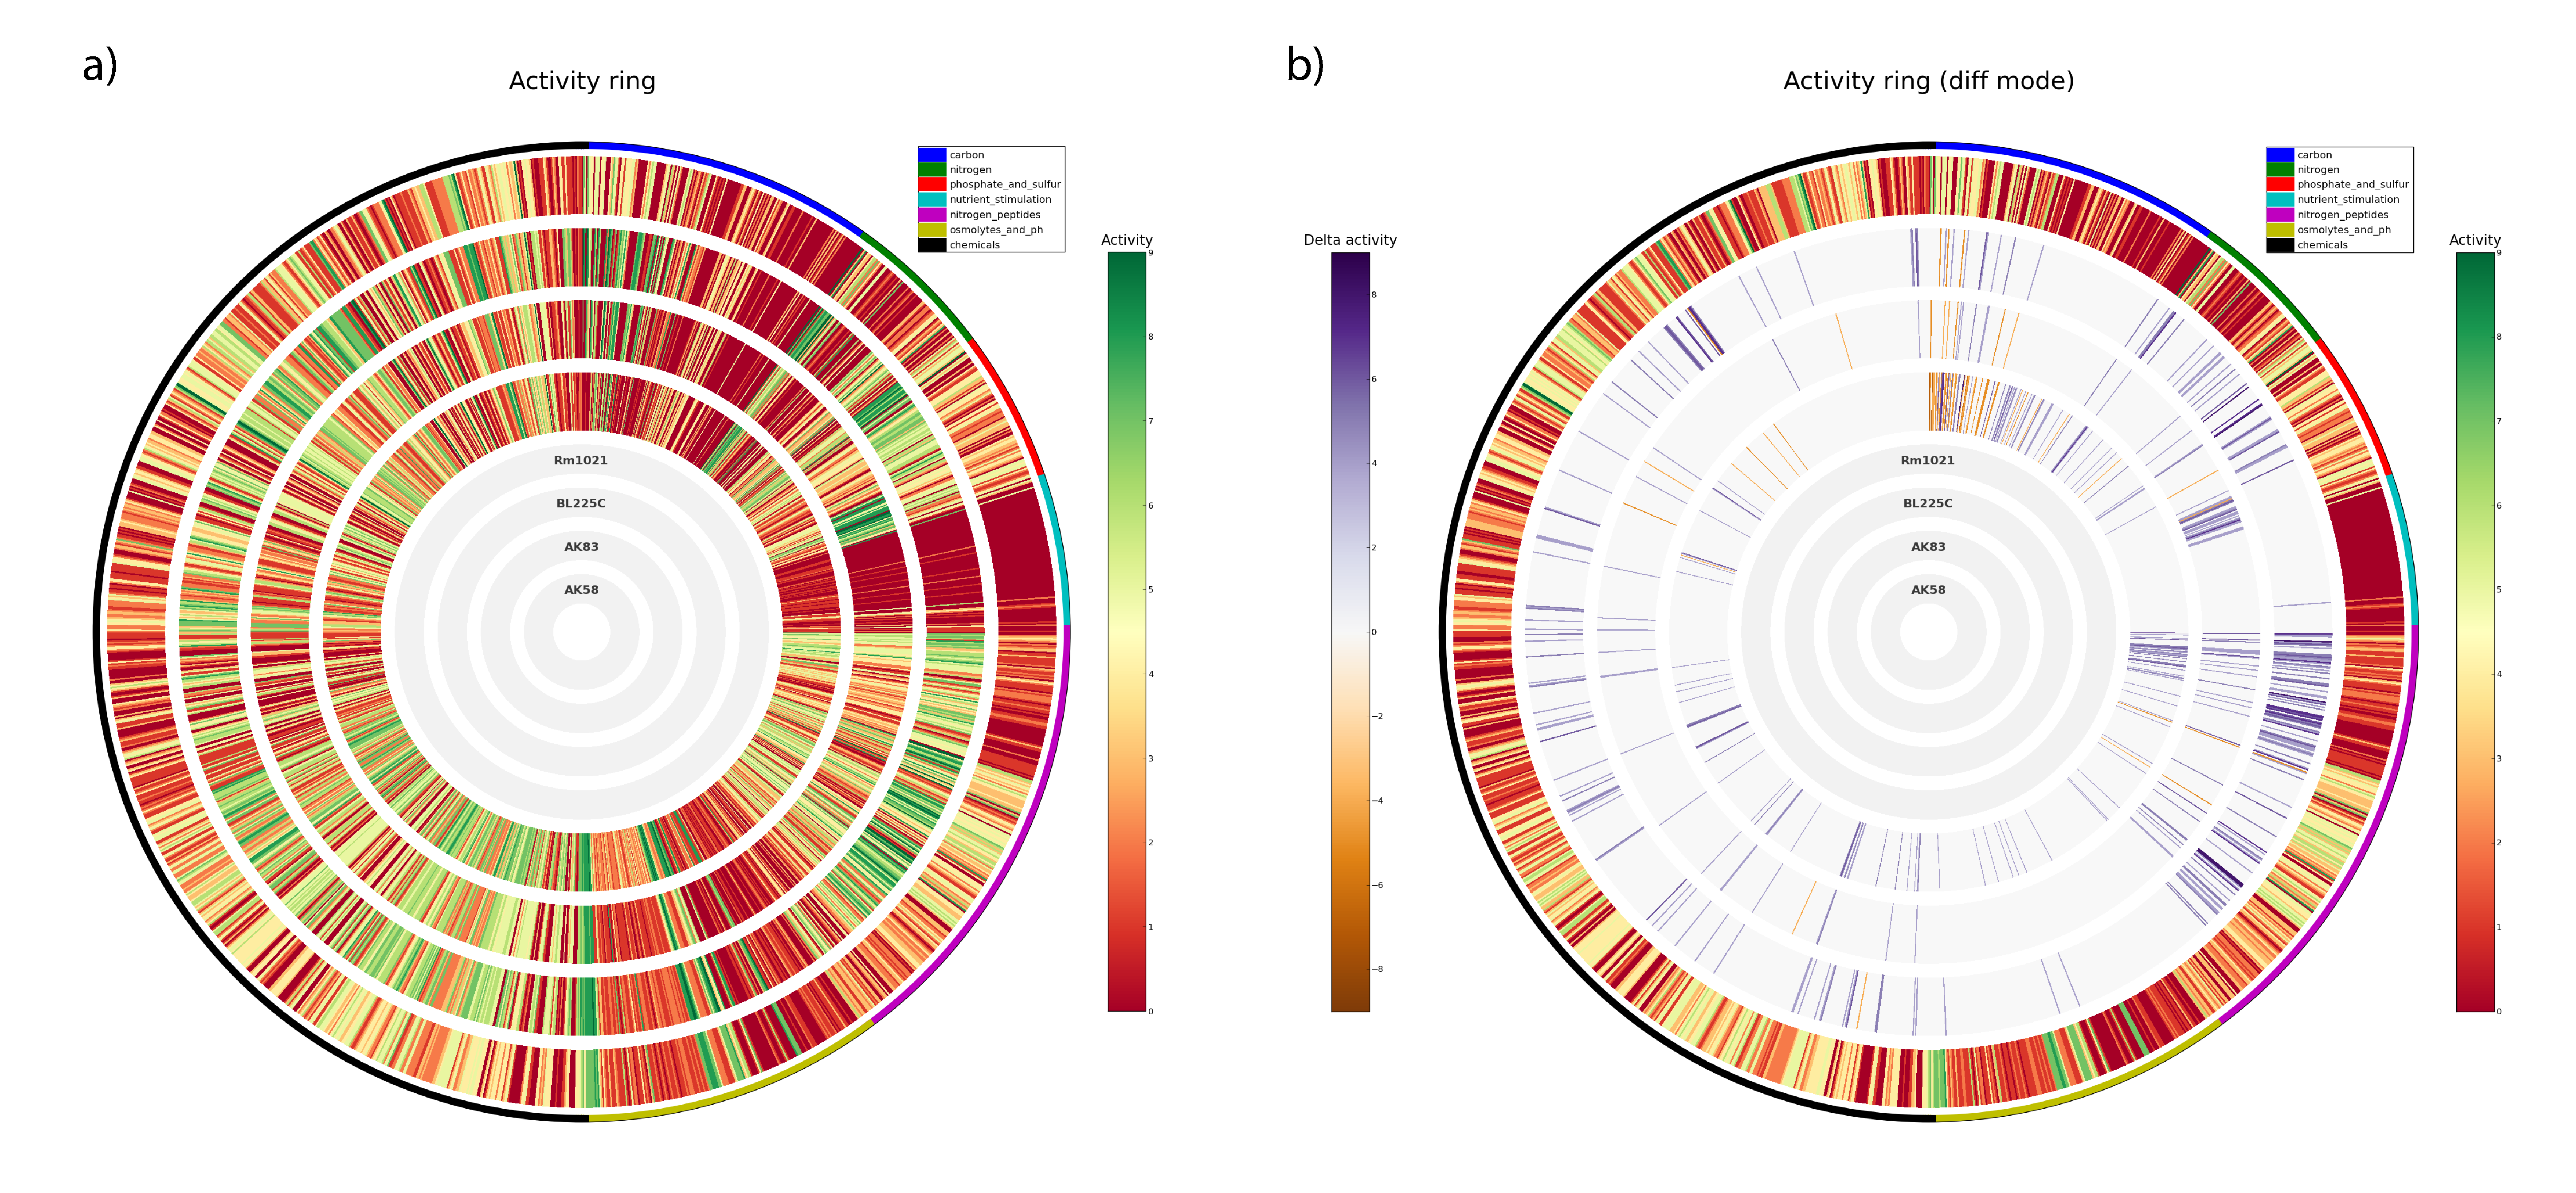
\includegraphics[width=1\textwidth]{figures/2/thesis_21a}
	\caption{\label{fig:drings}\textbf{Activity rings}\\
			Activity rings from \textit{S. meliloti} Phenotype Microarray data; grey inner circles indicate the strains order\\
			a) The Activity Index (AV) calculated for each strain and well is reported as a color going from red (0 AV) to green (9 AV)\\
			b) Diff mode: the difference with the AV value of strain Rm1021 is reported when equal or higher of 3 AV, grey otherwise; purple colors indicate an higher activity with respect to Rm1021, orange colors a lower activity}
\end{sidewaysfigure}

This second module allows the user to provide and manage any kind of phenomic data that can be linked to the KEGG compound database: a special focus is on PM data, for which a series of additional analysis tools are present, from raw data parsing to automatic activity calling and results plotting. In order to avoid any unreasonable or uninterpretable biological result displayed by using different parameters in certain situations and estimated to be up to 36\% of data \cite{vaas2012visualization}, for each well of the multiwell plate of the OmniLog\texttrademark system plate set, the \textit{Activity Index} (AV) is here proposed as a concise parameter based on the length of the lag phase, the slope of the curve, the average height, the maximum cell respiration and the area under the curve. Such index could provide both qualitative (presence/absence) and qualitative (model fitting data) information. First of all it is necessary to insert the output PM data from the Omnilog software: several files in csv format with raw data (in-cluded replicas) can be used. The program can then follow the steps below:

\begin{enumerate}
\item Parsing
\item Control signal subtraction
\item Signal refinement (smoothing)
\item Parameters extraction 
\item Activity Index calculation
\item Replica management
\item Growth curves plots 
\end{enumerate}

The data is parsed by the program and stored inside the project file; the user can then decide if the control signal has to be subtracted, or if a \textit{blank} plate (with no inoculants) should be used for this purpose, since some concerns regarding the control signal subtraction have been recently issued \cite{vaas2012visualization}. The PM curve parameters are extracted through the fit of one of three sig-moid functions (Logistic, Gompertz, Richards), reformulated to facilitate the parameters extraction \cite{zwietering1990modeling}; in order to avoid incorrect fittings or even failures, the growth curve signal is smoothed through the application of the Blackman window approach, as implemented in the SciPy package \cite{jones2001scipy}, which is also used to perform the actual fit. If all the three functions cannot be fitted to the PM curve, up to two more rounds of signal smoothing are applied; if the curve fit cannot be applied even after three rounds of smoothing, that particular well is classified as not active and the plateau, slope and lag parameters are set to zero.
The so-called Activity Index (AV) is a value between 0 and 9, which indicates those wells that exhibit low or none metabolic activity (0) and those with high metabolic activity (9) inside that par-ticular experiment: the AV parameter is calculated through a k-means clusterization (with k=10) on five growth curve parameters (max, area, height, lag, slope); the low activity growth curves will be assigned to the clusters with low AV, while wells exhibiting higher metabolic activity will be assigned to clusters with higher AV. The MeanShift clustering algorithm is also applied, in order to verify that there is a real clusterization of the growth curves in distinct clusters, as this algorithm has no fixed amount of clusters. The clusterization is performed with the scikits.learn package \cite{pedregosa2011scikit}. Since in most of the cases, many copies of each plates are used, there may be also the need to highlight those growth curves whose behavior is significantly different from the average: the program can search for those replica that are distant from the average AV (for that particular well and strain) more than an user-defined AV delta and flag them as \textit{purged}, meaning that they are not considered in the other analysis. The program has four replica purging policies, to help the user decide which PM curves have to be maintained. The last operation on the Phenotype Microarray data is the generation of PM curves plots with the matplotlib package \cite{hunter2007matplotlib}, which, compared to those generated by the machine vendor software, allow the comparison of more than two strains at the same time, with plate-wise plots, single wells plots and plate-wise AV heatmaps. Moreover it is also possible to display the entire metabolic profile of one or more strains in an interactive ring-mode view, called the “Activity ring”. Such graphical representation could report either the total Activity Index values (Figure \ref{fig:drings}a) or the metabolic differences between any selected sample versus the other strains by providing a "diff mode" Activity ring which displays the information by metabolic category of tested strain by using different colour intensity (Figure \ref{fig:drings}b). The values of the differences are represented by colour intensity (blue and orange parts indicate higher and lower values, respectively). Details of the Activity Index values are reported in a separate file which is directly accessible for the user. Different colors on the external line of the rings indicate different PM compounds categories. These visualizations allow an easier detection of the metabolic categories which are more variable in the tested strains. 

\subsubsection{DuctApe (dape)} 
The data gathered in the first two modules can be analyzed together in the third module of the DuctApe suite, which is designed to construct the metabolic network using the KEGG database information about reactions (which are the proteins mapped by the dgenome module) and compounds (which are the PM compounds, divided in categories); a series of interactive metabolic maps are then prepared, with specific color codes depending on the type of the experiment; the metabolic maps are encoded as a series of web pages that can be explored using a web browser. Using these maps, the user can highlight those pathways in which the gene pres-ence/absence pattern fits with the metabolic activity of the PM compounds. Moreover, thanks to the networkx module \cite{hagberg2008exploring}, several statistics can be computed for the whole reconstructed metabolic network and for each pathway, like the number of mapped reactions, the number and length of connected components (that are in fact distinct and independent metabolic modules) and the average AV for the total metabolic network and each pathway. Such analysis are useful for quick comparisons between various strains, moreover, the whole metabolic network graph is saved in gml format for further analysis on graphs visualization software like Gephi \cite{bastian2009gephi}.

\subsection{Results}
\subsubsection{Evaluation of dgenome on biological data}
\begin{figure}[!tb]
	\center
    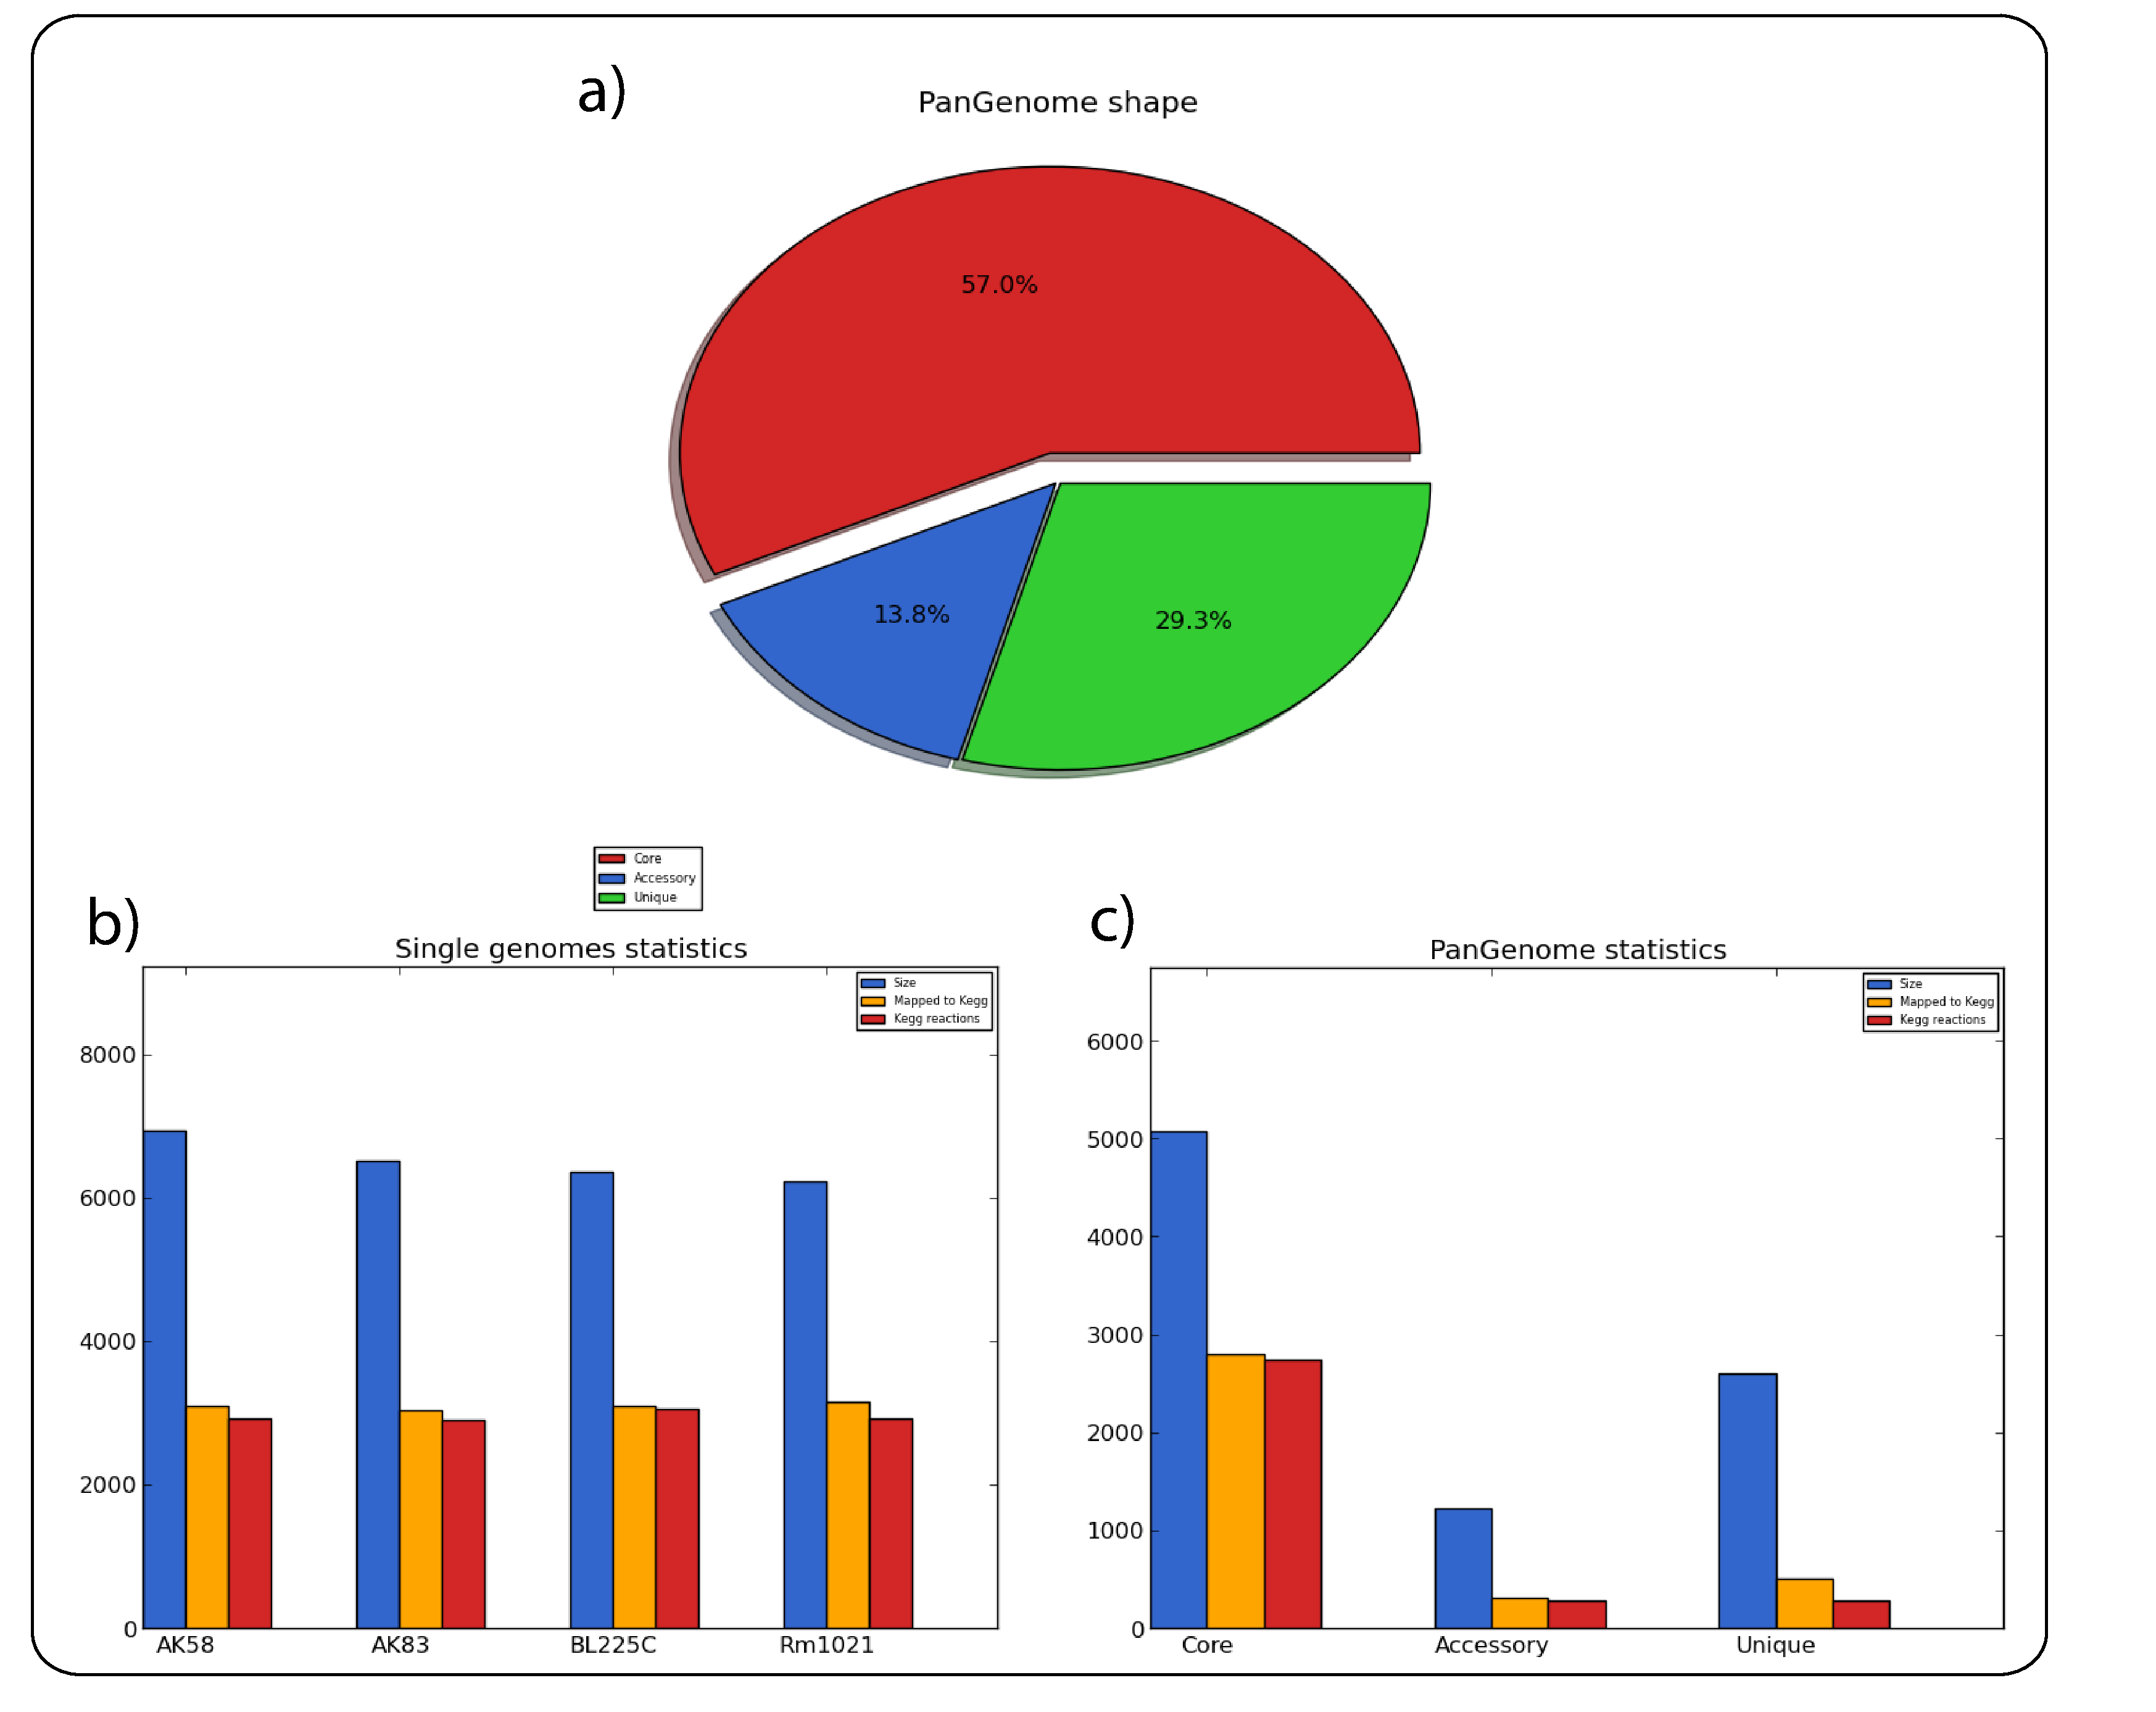
\includegraphics[width=0.9\textwidth]{figures/2/thesis_22}
	\caption{\label{fig:dgenome}\textbf{Pangenome statistics}\\
			a) The partition of the calculated pangenome in terms of core, accessory and unique genes\\
			b) Proteome sizes of the four S. meliloti strains and the fractions of proteins mapped to KEGG and KEGG reactions\\
			c) Pangenome partitions sizes in number of orthologous groups and fraction of orthologs mapped to KEGG and KEGG reactions}
\end{figure}

The four \textit{Sinorhizobium meliloti} strains used for this example study (Rm1021, AK83, AK58 and BL225C) were previously sequenced \cite{galibert2001composite}\cite{galardini2011exploring} and their predicted proteins were mapped to KEGG using the KAAS annotation web server, while the strains pangenome was computed thanks to the dgenome Blast-BBH algorithm; this resulted in a pangenome with 5074 orthologous groups belonging to the core genome, 1227 to the accessory fraction and 2606 unique to a single strain (Figure \ref{fig:dgenome}a). When looking at the number of proteins mapped to KEGG reactions, a similar number of proteins were mapped in each of the four genomes (Figure \ref{fig:dgenome}b), while when looking at the pangenome, the highest fraction of proteins mapped to KEGG come from the core genome, with a limited fraction of reactions mapped in the accessory and unique genome (Figure \ref{fig:dgenome}c).

\subsubsection{Evaluation of dphenome on biological data}
The first aim was to provide a rough evaluation of the Activity Index and its reliability. In order to do that the analysis and the comparison of the first PM dataset obtained from a previous experiment focused on 4 strains of the symbiotic model bacterium \textit{Sinorhizobium meliloti}: Rm1021, AK58, AK83, BL225C \cite{biondi2009metabolic} has been carried out. Such phenotipic dataset was obtained on the four strains by using the OmniLog\texttrademark system with plates PM1, 2, 3, 4, 9 and 10, and the metabolic variability was compared by means of the ratio between the average area and the area under the curve among strains for each condition. PCA and cluster analysis confirmed that the metabolic distance between Rm1021 and the other strains appeared to be quite consistent with the previous work, although it also provided slight differences involving strain AK58. In order to exploit the reasons of such differences, the Omnilog kinetic parameters of slope, maximum height, lag time and area under the curve were also individually analysed. Both PCA and cluster analysis confirmed that all the selected parameters, except the lag time, showed similar results as compared to the Activity Index which could thus be successfully applied as a unique parameter into the dphenome module (Figure \ref{fig:dpca}).

\begin{figure}[!tb]
	\center
    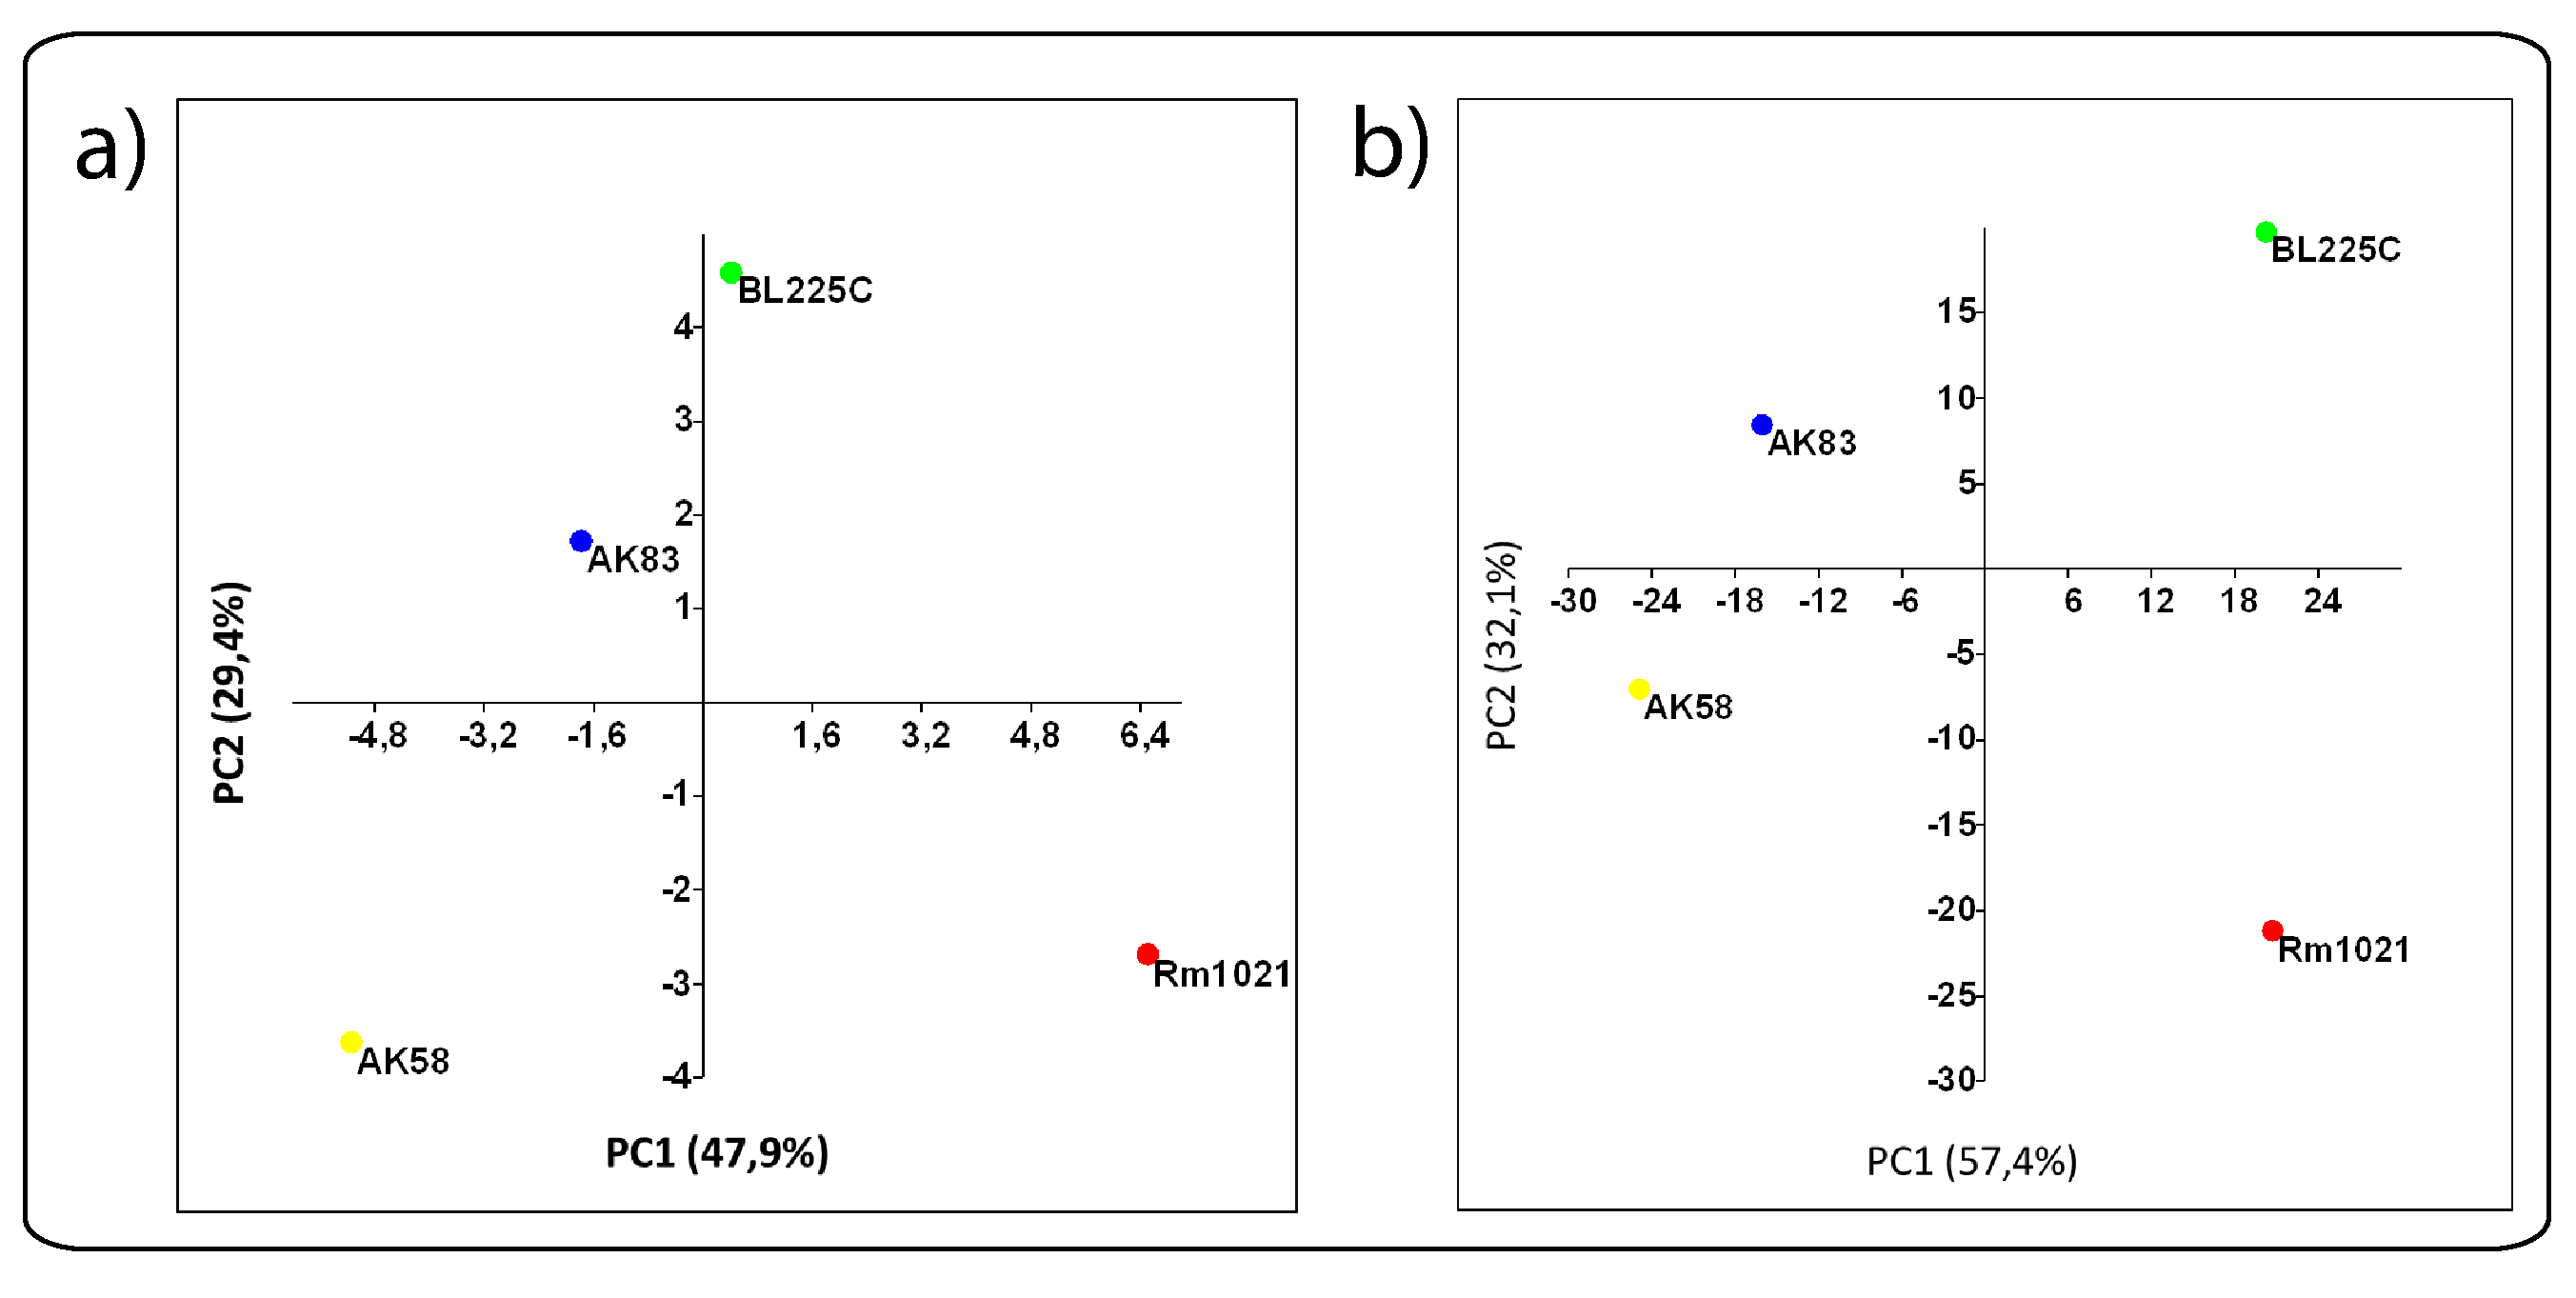
\includegraphics[width=1\textwidth]{figures/2/thesis_23}
	\caption{\label{fig:dpca}\textbf{Evaluation of the Activity Index by comparing the phenotypic diversity of four \textit{S. meliloti} strains}\\
			a) PCA results for PM profiles obtained from the analysis of 517 phenotypic attributes (dataset 2009) expressed as the ratio between the average area and the area under the curve among strains for each condition (see Biondi et al., 2009 for further details)
			b) PCA results for Activity Index values obtained from the PM analysis of the same 517 phenotypic attributes (dataset 2009)}
\end{figure}

\begin{table}[htbp]
  \centering
    \begin{tabular}{rcccc}
    \toprule
          & AK58  & AK83  & BL225C & Rm1021 \\
    \midrule
    More active & 57    & 26    & 70    & 4 \\
    Less active & 40    & 10    & 6     & 88 \\
    Total & 97    & 36    & 76    & 92 \\
    \%    & 5.1   & 1.9   & 4     & 4.8 \\
    \bottomrule
    \end{tabular}%
  \caption{\textbf{Unique metabolic functions of each \textit{S. meliloti} strain}}
  \label{tab:uniquemet}%
\end{table}%2


In order to evaluate the full potential of the dphenome module, the Activity Index was applied to a second phenotypic dataset obtained by a new biological test carried out using the entire OmniLog\texttrademark system PM plate set, and compared to the parameters calculated by the opmdata package \cite{vaas2012visualization}. We also compared the performances of the two approaches, with our parameters extraction taking up to ten minutes to be completed on the whole dataset (20 plates on 4 strains), while the opmdata package can takes up to several hours for the same task. A first qualitative output can be obtained by simply comparing the high/low metabolic activity on each PM well condition between the four strains. As shown in Table \ref{tab:uniquemet}, the 86,7\% of the substrates use was shared between the four strains (difference of Activity Index <3), whereas the 11,1\% of the metabolic repertoire was unique for each of them and could be strongly related to specific genomic traits. The remaining substrates were shared between more than one strain. The highest number of unique “more active” metabolic features was detected in PM plates inoculated with BL225C strain (70), suggesting a higher metabolic potential of this strain as compared to the other three. In fact, the BL225C strain exhibited “less active” phenotypic traits in 6 conditions only. In contrast, the Rm1021 strain seems to be the less metabolically competitive between the four strains, as it showed the lowest number of “more active” metabolisms (4) and the highest number of “less active” metabolisms (88). When looking at the single PM compound categories (Table \ref{tab:ductcateg}), trends highlighted in Table \ref{tab:uniquemet} are confirmed for each category, with strain Rm1021 as the less active in each cate-gory, except for  plates measuring the tolerance to pH and stresses, in which strain AK83 has a lower proportion of active wells com-pared to strain Rm1021.

\begin{sidewaystable}[htbp]
  \centering
  	\begin{tabular*}{\textwidth}{rccccrr}
    \toprule
    \multicolumn{1}{c}{} & \multicolumn{4}{c}{Active wells (\%) *} &       &  \\
    \midrule
    Category & AK58  & AK83  & BL225C & Rm1021 & \multicolumn{1}{c}{Average difference} & \multicolumn{1}{c}{Main differences (\%)** } \\
    Carbon & 14,1  & 20,8  & 22,9  & 14,1  & \multicolumn{1}{c}{1,7} & \multicolumn{1}{c}{22,9} \\
    Nitrogen & 40,6  & 25    & 51    & 19,8  & \multicolumn{1}{c}{1,3} & \multicolumn{1}{c}{5,2} \\
    Phosphate and sulfur & 29,2  & 43,8  & 66,7  & 14,6  & \multicolumn{1}{c}{1,9} & \multicolumn{1}{c}{12,5} \\
    Nutrient stimulation & 1     & 4,2   & 2,1   & 1     & \multicolumn{1}{c}{0,4} & \multicolumn{1}{c}{1} \\
    Nitrogen peptides & 40,6  & 28,5  & 62,8  & 14,6  & \multicolumn{1}{c}{1,7} & \multicolumn{1}{c}{9} \\
    Osmolytes and pH & 25,5  & 17,7  & 22,4  & 19,8  & \multicolumn{1}{c}{0,9} & \multicolumn{1}{c}{1,6} \\
    Chemicals & 41,9  & 39,8  & 47,6  & 17,9  & \multicolumn{1}{c}{1} & \multicolumn{1}{c}{2,8} \\
    \bottomrule
   \end{tabular*} 
  \caption{\textbf{Phenomic data for each Phenotype Microarray compound category}\\
  \textbf{*} compounds for which the AV (activity index) is equal or over 5\\
\textbf{**} compounds for which the average difference between the strains is equal or over 3 AV (activity index)}
  \label{tab:ductcateg}%
\end{sidewaystable}

However, in order to further highlight any metabolic difference between the selected samples it could be also possible to compare the Activity Index of the curves over time. The total metabolic differences of the entire PM dataset was then displayed as an Activity Ring (Figure \ref{fig:drings}a). It could be also visualized as diff mode in order to visually detect any difference in higher/lower metabolic reaction between any selected strain and the other samples. For instance, in Figure \ref{fig:drings}b the relative metabolic differences between Rm1021 and the other strains are shown; a significant increase of blue colour intensity appeared in the “Nitrogen peptides” category, suggesting a lower metabolic activity of Rm1021 as compared to the other \textit{S. meliloti} strains. Thus, the user is free to get further information by accessing a separate file, where the detailed values of Activity Index for each substrate are reported.

\subsubsection{Evaluation of DuctApe on biological data}
\begin{sidewaysfigure}
	\center
    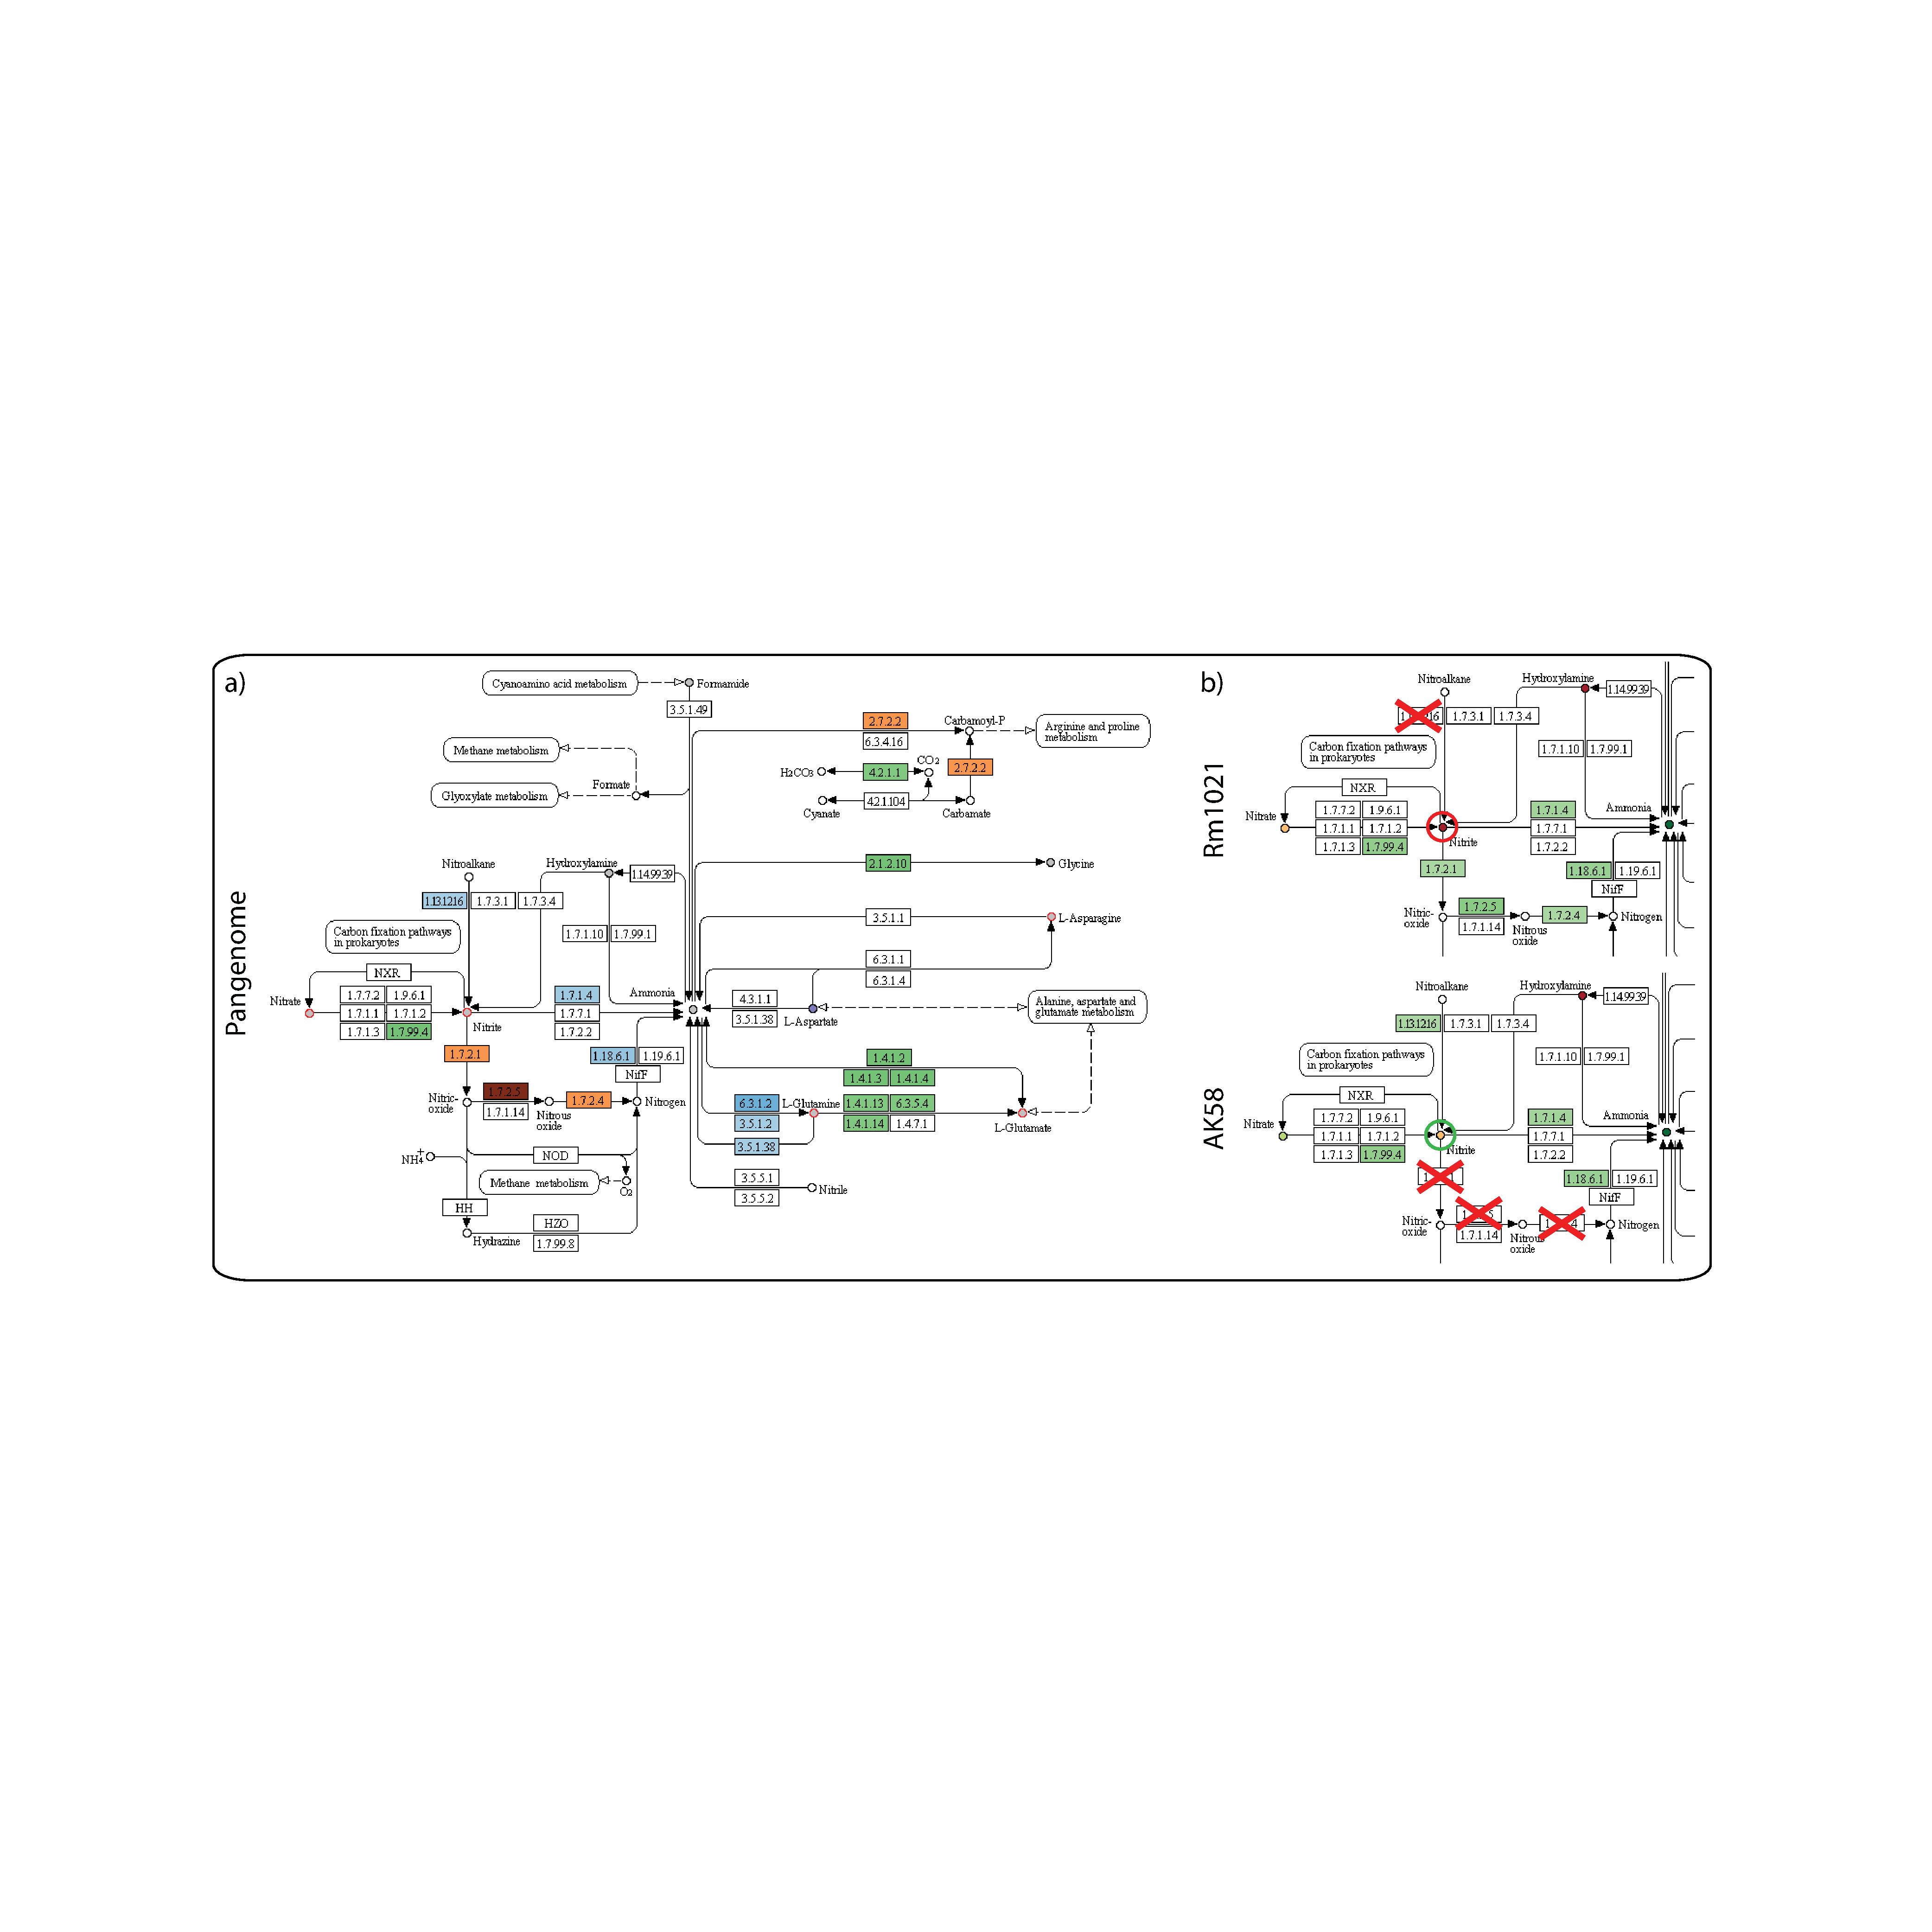
\includegraphics[width=1\textwidth]{figures/2/thesis_24}
	\caption{\label{fig:dkeggmaps}\textbf{Metabolic network analysis on the \textit{S. meliloti} pangenome}\\
			Boxes represent reactions, with color intensity proportional to the copy number, while circles represent compounds\\
			a) Pangenome metabolic map of nitrogen metabolism: core reactions are colored in blue, reactions present both in the core and accessory genome are colored in green, unique reactions are colored in orange; compounds are colored in purple when the mean AV difference in the four strains is equal or higher of 3 AV, grey otherwise. Red circles around grey compounds highlight those compounds for which at least one strain has an AV difference with the other strain equal or higher than 3 AV\\
			b) A section of the same metabolic map in strain Rm1021 and AK58: reactions are colored in green, compounds are colored according to their AV (as in Figure \ref{fig:drings}); differences between the two strains are highlighted with red crosses}
\end{sidewaysfigure}

The schematic representation of the metabolic pathways potentially expressed from each of the four strains was retrieved by selecting the command "dape map". A number of metabolic maps from KEGG database were separately displayed as functional categories for each strain. The different gene-related phenotypes could be analyzed on the basis of the presence of genes and substrates of each map, highlighting them with different colors (as described in Figure \ref{fig:dpca}). However the potentials of DuctApe could be fully expressed in case the user wants to compare the metabolic features of multiple samples. For example in Figure \ref{fig:dkeggmaps}a the pangenomic map for nitrogen metabolism (map n. 00910 of KEGG database) is shown. Although most of the reactions are catalyzed by proteins encoded by genes which were not retrieved from the genomic data (white boxes), some reactions appeared to be controlled by genes of the core genome (blue) or present in both core and dispensable genome (green). Nevertheless, four orange boxes indicated the presence of the following functional genes located on the dispensable genome: nitrite reductase (reaction 1.7.2.1), nitrous-oxide reductase (reaction 1.7.2.4) and carbamate kinase (reaction 2.7.2.2). This means that these functions are not shared between all  strains. In fact those genes were not detected in AK58 and AK83 strains. Similarly, most of the metabolic substrates involved in the nitrogen cycle are not included into the PM microplates set (white circles) but several substrates could be used (or not) by the four strains (colored circles). For instance, all the samples showed active metabolism for some specific substrate (i.e. Ammonia, L-Glutamate, etc.) as well as no active metabolism for some other substrate (i.e. Hydroxylamine, Formamide, etc.) which are indicated with a grey circle on the map. The red border of circles related to some substrates (i.e. Nitrite, Nitrate, etc.) indicated that the four strains differently used those specific substrates and that the Activity Index values differed for more than 3 units. The simultaneous visualization of both genomic and phenomic information allowed linking the use of nitrite with the presence of nitronate monooxygenase (reaction 1.13.1216) in AK58 strain, whereas the presence of nitrite reductase (reaction 1.7.2.1), nitrous-oxide reductase (reaction 1.7.2.4) and carbamate kinase (reaction 2.7.2.2) appeared to be not enough to directly drive the nitrite catalysis in Rm1021 and BL225C strains, at least under these experimental conditions (Figure \ref{fig:dkeggmaps}b).

\subsection{Discussion}
Although genomics is continuously living a tremendous development, both on the technical and computational sides \cite{metzker2009sequencing}, a high-throughput ”phenomics” analysis, is developing, based for instance on Omnilog PM technology. Similarly to genomics, the huge amount of PM data generated by single experiments needs to be analyzed through a suitable bioinformatic tool in order to unravel all the potential features of the data expressed by curve shapes which are produced by microbial respiration. Moreover, in a systems biology framework, it is compulsory also to be able to try to correlate microbial genotypes and phenotypes. Our results enabled to propose DuctApe as a user-friendly solution for the visualization of PM data, the exploring of both the genomic information and the phenotypic expression of microbial cells, providing also comprehensive insights into their correlation with cellular metabolism. Actually, the main available computational tools for PM data analysis are completely or partially missing such functions. For instance, the original Omnilog\texttrademark PM software provides only limited functionality for data analysis, especially if more than two or more curves are compared, and the most common alterna-tives, such as PhD database \cite{li2005phd}, the RetroSpect\texttrademark software \cite{biolog2008} and PheMaDB \cite{wenling12phemadb}, are mainly customised databases which can support the management of data and report generation, but provided only limited functionality for both visualization and analysis of kinetic curves. 
The dgenome module implements functionalities that were already available in other tools, such as KAAS \cite{moriya2007kaas} for the metabolic reconstruction and InParanoid \cite{ostlund2010inparanoid} for the orthology algorithm; the real innovation posed by this module is the ability to easily obtain and organize data, as well as making them available to the dape module for the final metabolic network reconstruction. The pangenome construction algorithm is designed to be parallelizable, allowing a faster analysis in systems with many CPUs available. As demonstrated here, the dphenome module represents the first innovation of the DuctApe suite. The tool provides an automated classification and identification of the PM curves and applies the Activity Index as unique comprehensive kinetic parameter for the computational high-throughput processing of the raw data. In fact, although the gathering of kinetic parameters of PM curves into a single index was already used for analysing PM datasets and comparing the metabolic profile of different bacterial strains  \cite{biondi2009metabolic}, the Activity Index here proposed is a single and reliable value that includes the whole information of the curve shapes, going far beyond the mere presence/absence paradigm or the partial evaluation of the metabolic reactions based on the parametric analysis tool of the native Omnilog PM software. In fact, such parametric analysis method is based only on few data points of the curve shapes, thus consistently reducing the biological information content of each experiment, as recently reported \cite{vaas2012visualization}. The Activity Index value is based on the combination of parameters which are calculated by the measurement of all data points of the curve. In fact, for a comprehensive comparison of the PM curves several parameters have to be considered to get a meaningful biological estimation. Although a raw combination of few curve parameters into a single one is expected to introduce biases, we took into account that the combination of 4 or 5 parameters could reduce the load of the “correlated” parameters (i.e. area and average height) and at the same time emphasize the biological information. In order to validate the approach used to calculate the Activity Index, we compared our curve parameters extraction method with those obtained on the same dataset by applying the approach described by Vaas and colleagues, seeing only limited and no significant differences due to the curve smoothing algorithm used by dphenome. Hence, the Activity Index can be considered as a useful and reliable tool able to automatically calculate the metabolic activity of a large number of samples, replacing the application of more sophisticated multivariate data analysis. The use of a single value with a definite range to discriminate the metabolic activity inside the experiment allows an easier analysis and an easier embedding of the phenotypic data inside the metabolic maps. Although any statistical analysis of the metabolic differences of the tested strains is beyond the scope of this study, considering the very low replicate number usually reported in PM experiments (especially if the entire OmniLog\texttrademark PM plate set is used), the proposed modules can provide useful biological indications to be validated in subsequent specifically designed experiments; however, the dphenome module allows the user to automatically exclude the replicas with inconsistent activity. The evaluation of the Activity Index on the first PM dataset did not provide significant differences as compared to the old results calculated with the multiplication of Area and slope values, as shown in Figure \ref{fig:dpca} (see also Figure 2b in the work of Biondi and colleagues). Quick and informative visualization of the Activity Index values of the selected strains can be easily achieved by using the appropriate Activity rings command while, at the same time, retaining the possibility of getting deeper insights into more detailed metabolic categories and substrates. This kind of graphical representation is particularly suitable when facing huge and complicated datasets such as the ones obtained from the entire PM plate set on two or more bacterial strains. Actually there is not any other software available to perform such task, excepted the R-based tool presented by Vaals and co-workers (2012) which, however, appeared to be more suitable for analyzing just one microplate data (i.e. GEN III microplates\texttrademark), than the more comprehensive metabolic profiles provided by the entire OmniLog\texttrademark system plate set (PM 1-20). In fact although opmdata tool presents the possibility to compare more than two samples at a time, the PM curve outputs provided by such R tool are shown as heat-maps or 8x12 grid-like layouts. This visualization appears to be quite convenient and helpful to display the curve kinetics of two or more samples on a limited number of metabolic conditions, but completely inappropriate for the comparison of a high number of plates containing thousands of different substrates (i.e. PM 1-20). Moreover, thanks to the single measure of the Activity Index, the metabolic activity can be represented with just one color, making the comparison between experiments easier. The dape module represents another innovation of the software suite and, at the best of our knowledge, it represents the first tool which allows the user to link and visually analyse both genomic and phenomic high-throughput datasets. Although a first tentative to manually link the PM data to genomes by comparing the metabolic pathways of several carbohydrates used by two \textit{Bacillus cereus} strains has been reported \cite{mols2007metabolic}, DuctApe allows the user to automatically do it for all the metabolic pathways present in the KEGG database, together with the analysis on the whole metabolic network reconstruction though the calculation of metabolic networks statistics.
The idea of using the KEGG database and the development of such tool came from the native OminoLog\texttrademark PM software which enables the user to identify a single substrate of any PM microplate linking the displayed picture to the KEGG database. However, the dape module extremely improved the link between PM data and the KEGG database, allowing the users to simultaneously assess any metabolic feature of all the substrates of the entire PM plate set and, moreover, integrate this information with the genomic data. This kind of data processing will most probably enhance data modelling of genome-wide metabolic pathway and gene annotation.
Although each module of the DuctApe suite can be also used independently from each other, their integration and the use of the dape module allows the user to really get into a first reliable biological evaluation of the results. Further work is still necessary to optimize the integration of genomic and phenomic data; in fact, as DuctApe is based on the KEGG platform, the number of the possible genomic explanations of a specific phenotypic feature is strongly limited either by the KEGG database itself (i.e. the available microbial metabolic pathways are basically obtained by few model-strains, such as E. coli) and by the number of substrates which are accessible on PM plates. Furthermore it is well known that the phenotypic diversity of a cell is most likely affected by regulatory factors or genetic differences that are not detected by PM system (i.e. transport proteins, receptors, etc.) and differences in transcriptional regulation might explain any metabolic incongruity. Thus, a more reliable correlation between genome and phenotypic features should take into account the transcriptome information as well. Finally, although some methods have been already proposed \cite{vaas2012visualization}, further work is necessary to optimize both the parameter estimation and the statistical assessment of the detected metabolic differences and an additional statistical analysis tool could be added to the DuctApe suite.


%%-----------
%% Backmatter
%%-----------
\backmatter
\chaptermark{Bibliography}
\renewcommand{\sectionmark}[1]{\markright{#1}}
\bibliographystyle{unsrt}                           %Use alpha codes for references
\sectionmark{Bibliography}
\addcontentsline{toc}{chapter}{Bibliography}        %Force addition of Bibliography to TOC    
\bibliography{References}								

\mainmatter

%%%%%%%%%%%%%%%%%%%%%%%%%%%%%%%%%%%%%%%%%%%%%%
\logvartrue
\chapter{A shared toolbox}
%%%%%%%%%%%%%%%%%%%%%%%%%%%%%%%%%%%%%%%%%%%%%%
\label{chap:alpha}

\section{Common genetic basis for bacterial association with plants}
The plant-bacteria association is indeed a complex interaction, with many possible mechanisms, each one with distinct effects on plant physiology and agriculture (see section \ref{atale2cities}). The various kinds of plant association (endophytism, symbiosis, pathogenicity) are found in many bacterial taxa, with some well-documented examples of bacterial species able to exhibit more than one distinct kind of association with plants \cite{bashan2004azospirillum} \cite{chi2005ascending}; the most studied phylum of bacteria associated with plants belongs to the \textit{Proteobacteria} phylum, with the classes of \textit{alpha}, \textit{beta} and \textit{gamma}-\textit{proteobacteria} as the most studied, especially for the symbiotic nitrogen fixing phenotype. Given the high variability in the association phenotypes and the different mechanisms and signals exchanged, the genetic determinants of such complex interactions are most likely a vast repertoire of many genes, many of which may be not shared across the various taxonomical entities able to interact with plants. Understanding if a common shared set of genetic elements for the interaction with plants exists inside the bacterial kingdom is crucial for both evolutionary and functional studies: on the evolutionary perspective, the origin and dynamics of the plant association genotypes may be derived to gain a more precise history of mutualism/symbiosis, both with plants and more generally with higher organisms. The functional perspective, however, is the one that would have the biggest impact on agriculture, because such shared genetic elements will most probably be key factors in the plant interaction mechanism, and may form the basis for genetic engineering experiments to test their specific role in the plant interaction phenotype.

\subsubsection{Comparative genomics of distant species}
When applied on large heterogenic datasets, the comparative genomics analysis becomes more complex: the presence of different evolutionary distances between each genome is challenging for the orthology assessment step, mostly because an higher evolutionary distance often implies a smaller sequence similarity, which may not be detectable by the Blast algorithm \cite{kim2007clustering}. Another problem posed by comparative genomics analysis on heterogenuos datasets is the presence of species that have experienced a strong genomic reduction, such as obligate symbionts and intracellular pathogens; with the relaxation of evolutionary constraints due to the pathogenic or symbiotic lifestyle, many genes are lost to improve the replication efficiency and speed (see for instance \textit{Buchnera aphidicola}, the obligate endosymbiont of aphids \cite{tamas200250}). As a consequence of this genomic reduction, the presence of these genomes would exclude many otherwise conserved genes from the so-called \textit{core} genome: the exclusion of such genomes is therefore a prerequisite for large comparative genomics studies. Being an interesting functional and evolutionary subject for computational experiments, many algorithms have been developed to perform comparative genomics analysis on a large taxonomical scale: such techniques may involve the use of the information on the phylogenetic relationships between each species to tune the homology search cut-offs \cite{rehmsmeier2001phylogenetic} \cite{qian2003detecting} \cite{qian2004performance}, the use of the protein domain content together with sequence similarity \cite{qian2003detecting} \cite{qian2004performance} \cite{hollich2007pfamalyzer} or the relaxation of the homology cut-offs in order to consider all the homology signals, then clusterized to extract the orthologous families \cite{kim2007clustering}.

\newpage
\section{Plant-bacteria association and symbiosis: are there common genetic traits in \textit{Alphaproteobacteria}?}
The plant association phenotype is a common functional feature inside the class \textit{Alphaproteobacteria}, were many species able to interact with plants either through endophytism, symbiosis or pathogenicity can be studied. Even if the genetic elements needed for a successful symbiosis are well-known, little is known about their occurrence in all the alphaproteobacterial tree, as well as little or no information is available regarding the presence and occurrence of genes necessary to establish an endophytic interaction with a plant. A comparative genomics study on 92 genomes belonging to the alphaproteobacterial class has been carried out to highlight the core genome of this taxa, as well as the conserved genetic elements needed for endophytism and symbiosis, if present. The dataset comprises species that are plant symbionts, endophytes or species that are not associated with plants, with the exclusion of obligate pathogens and other species with reduced genomic sizes. Insights on evolutionary dynamics and phylogenetical distribution of this shared genes has also been analyzed and discussed.

\newpage
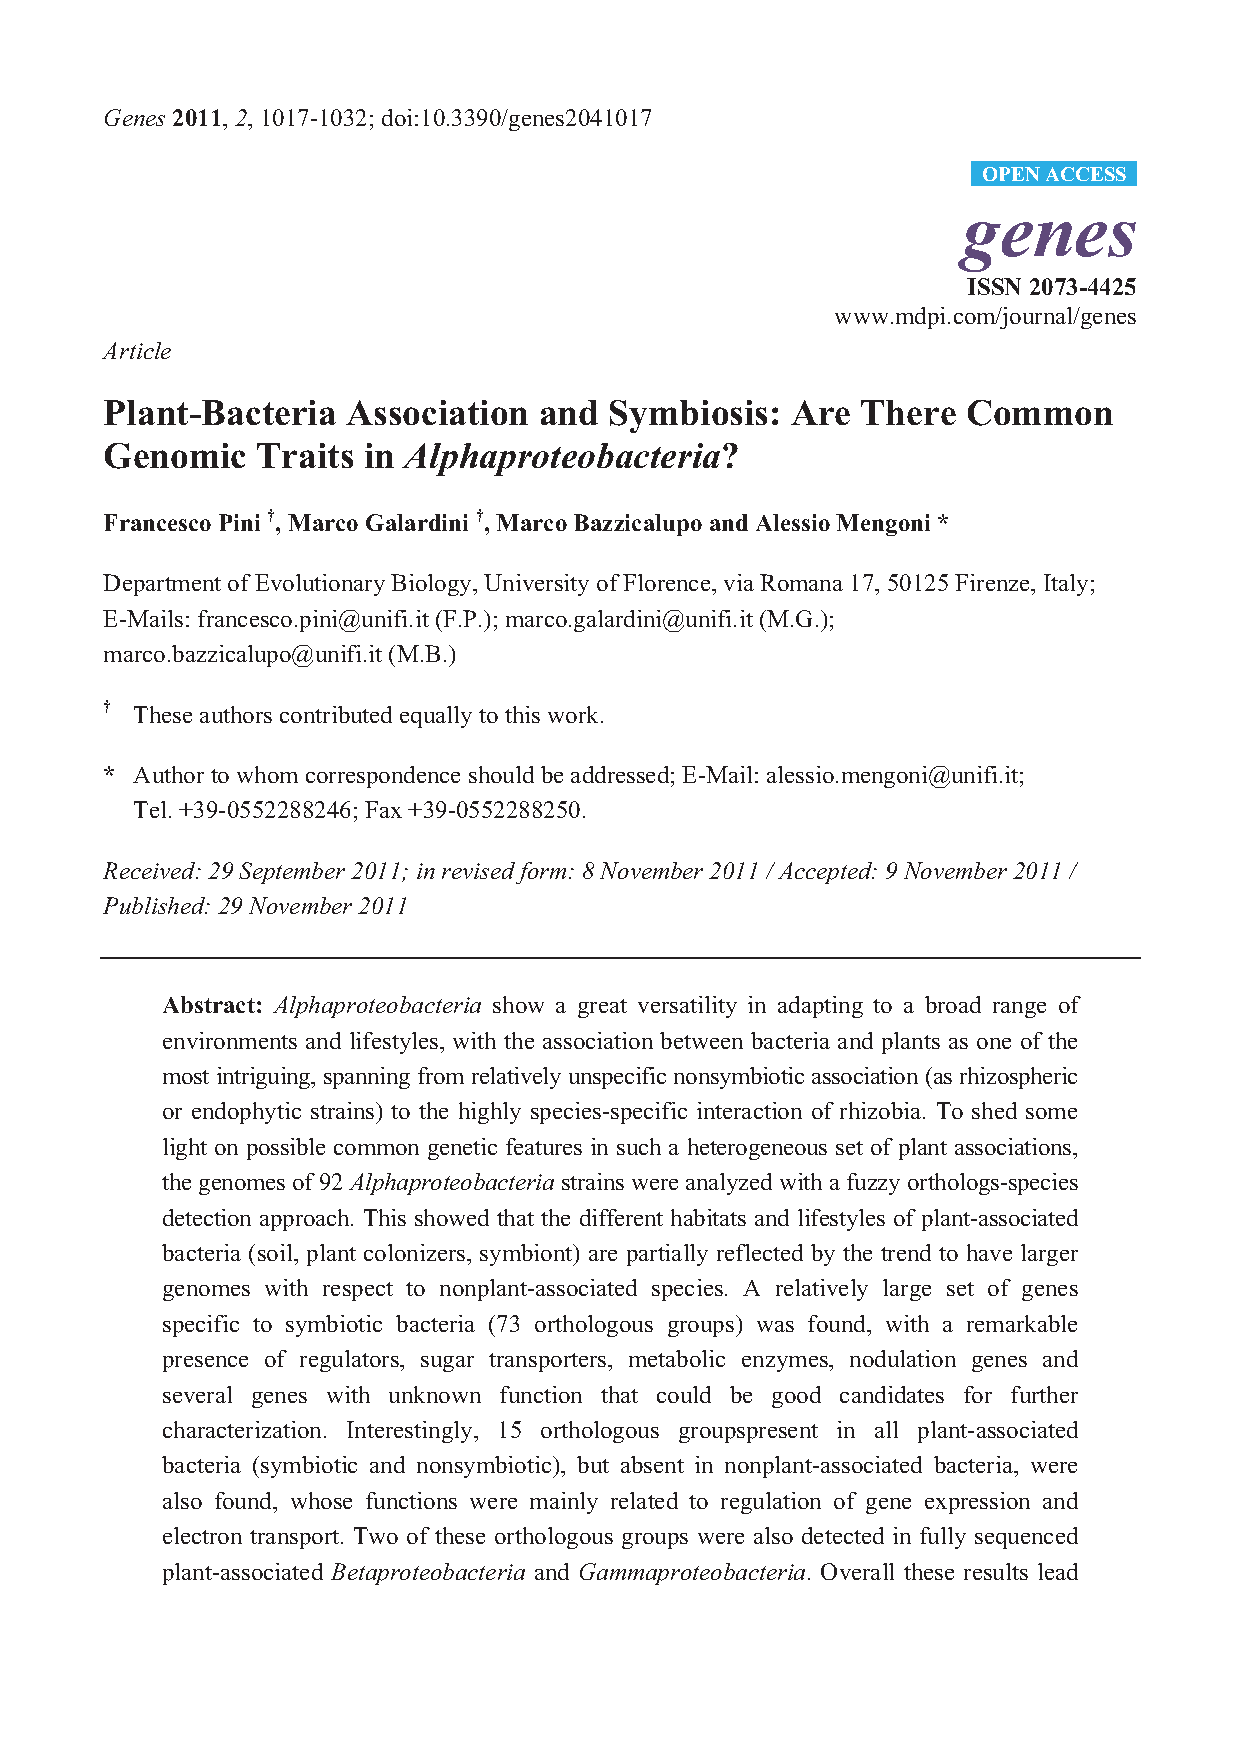
\includepdf[pages=-,offset=10mm 0, scale=0.9]{articles/Pini2011.pdf}
\newpage

%%-----------
%% Backmatter
%%-----------
\backmatter
\chaptermark{Bibliography}
\renewcommand{\sectionmark}[1]{\markright{#1}}
\bibliographystyle{unsrt}                           %Use alpha codes for references
\sectionmark{Bibliography}
\addcontentsline{toc}{chapter}{Bibliography}        %Force addition of Bibliography to TOC    
\bibliography{References}									

\mainmatter
%%%%%%%%%%%%%%%%%%%%%%%%%%%%%%%%%%%%%%%%%%%%%%
\logvartrue
\chapter{The quest for the super-rhizobium}
%%%%%%%%%%%%%%%%%%%%%%%%%%%%%%%%%%%%%%%%%%%%%%

\section{Comparative genomics of \textit{S. meliloti}}
As shown in chapter \ref{chap:alpha}, inside the class Alphaproteobacteria there is a common genetic "toolbox" for the establishment of plant symbiosis; however, little is known about the intraspecific variability of the genes related to symbiosis and its relationships to the observed phenotypic variability, especially in the plant growth promotion phenotype. Up to date, only one strain of the nitrogen-fixing bacterium \textit{Sinorhizobium meliloti} was available \cite{galibert2001composite}, with a limited possibility to perform comparative genomics studies, even though experimental approaches like the Comparative Genomics Hybridization arrays (CGH) have been performed on four natural strains of \textit{S. meliloti}; about 5\% of the genes of this genome was found to be variable in the natural isolates of this species and the megaplasmid pSymA was found to be the hotspot for intra-specific differentiation, with the variable regions mainly grouped as clusters \cite{giuntini2005large}. The peculiar genomic composition of the \textit{S. meliloti} species, having three replicons, is also an interesting feature to be studied through comparative genomics, to understand if there is also a variability in the size of these replicons, on functional content and on their structure; thanks to the recent advances in sequencing technologies, the complete or draft genomic sequences of other natural isolates of this species have been sequenced: their genomic features with regard to plant symbiosis, nitrogen fixation and genome evolution are discussed in this chapter.

\newpage
\section{Exploring the symbiotic pangenome of the nitrogen fixing bacterium \textit{Sinorhizobium meliloti}}
The first comparative genomics analysis on the \textit{Sinorhizobium meliloti} species has been performed on the reference laboratory strain Rm1021 and two natural isolates: one from the Aral sea region, in Kazakhstan (strain AK83) and one from an agricultural field from Lodi, Italy (BL225C); their 
variability in the symbiotic phenotype has been already established \cite{biondi2009metabolic}. The presence of such an high variability should then be reflected in a different pattern of presence/absence of genes related to symbiosis, some of which may have been not yet characterized; regulatory features may also be related to the different observed phenotypes, as shown in a comparative genomics study of the cell cycle in \textit{Alphaproteobacteria} \cite{brilli2010diversity}.

\newpage
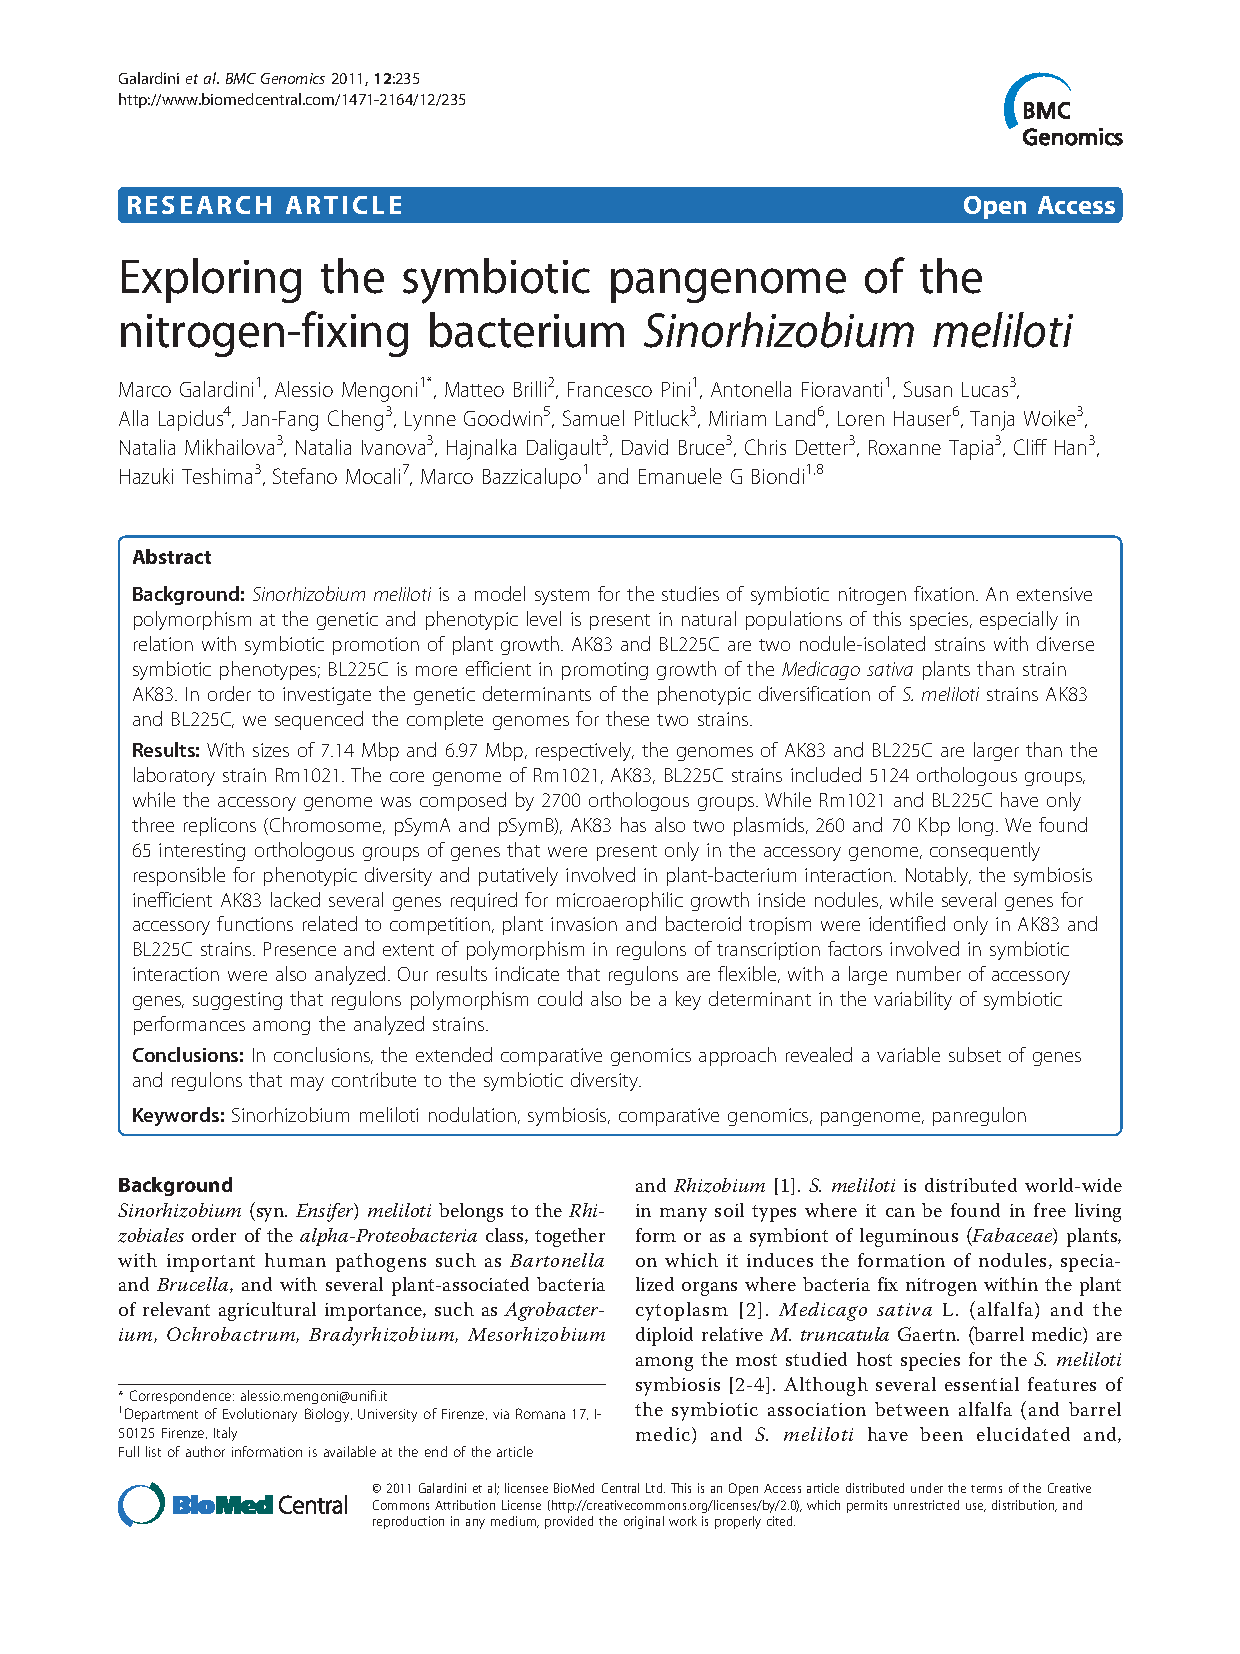
\includepdf[pages=-,offset=10mm 0, scale=0.9]{articles/Galardini2011.pdf}

\newpage
\section{Replicon-dependent bacterial genome evolution: the case of \textit{Sinorhizobium meliloti}}
Many bacterial species, such as the alphaproteobacterium \textit{Sinorhizobium meliloti}, are characterized by open pangenomes and strains contain multipartite genomes consisting of a chromosome and other large-sized replicons, such as chromids, megaplasmids and plasmids.
The evolutionary forces that shape the pangenome of species with multipartite genomes in both functional and structural aspects are still poorly understood. To shed light on this topic, we sequenced the genomes of ten \textit{S. meliloti} strains, which were combined in our analysis to four publicly-available additional genomic sequences.
Results obtained indicated that the three main replicons present in these strains (a chromosome, a chromid and a megaplasmid) show a partly independent history during strains differentiation. In particular, the chromid was shown to be a hotspot for positively-selected genes and, unexpectedly, genes resident in the chromid were also found to be more widespread in distant taxa than those located in the other replicons. Moreover, through the exploitation of a DNA proximity network, a series of conserved “DNA backbones” were found to shape the structural evolution of the genome, with the rest of the genome experiencing rearrangements. 
The presented data allow to depict a scenario where the evolution of the \textit{S. meliloti} pangenome includes a structurally-conserved genome fraction that evolves by positive selection (mainly on the chromid), and a highly-variable fraction, that mostly contributes to structural fluidity and to the emergence of new functions (the megaplasmid), then suggesting that the chromids could have had a distinctive role in intra-species differentiation\footnote{Authors: \textbf{Marco Galardini}, Francesco Pini, Marco Bazzicalupo, Emanuele G. Biondi, Alessio Mengoni}.

\subsection{Introduction}
The relative contribution of the forces that drive the evolution of organisms and genomes and the coupling between genome and phenome evolution have focused the attention of several investigators and lead to the formulation of new hypotheses on adaptive traits \cite{hughes2011evolution} and to the identification of possible rules governing the evolutionary process at large phylogenetic scale \cite{koonin2010constraints}. Concerning the evolutionary processes at the intra-species scale (\textit{microevolution}), prokaryotic organisms follow distinct patterns with respect to eukaryotic organisms. In particular, it is well known that, even in the same species, bacterial genomes of different strains often present a core and a dispensable genome, the core genome being common to all strains, while the dispensable genome comprises genes present only in one (unique) or in a subset of strains (accessory) \cite{tettelin2008comparative}. The dispensable genome, which can account for a large fraction of the entire pangenome, has been shown to harbor gene related to local adaptation functions, originated by relatively recent horizontal gene transfer events \cite{medini2008microbiology} and it may explain phenotypic differences found in natural strains \cite{biondi2009metabolic}; by looking at the proportion of the dispensable fraction over the core genome, it is also possible to speculate about the life-style of a given species \cite{tettelin2008comparative}. Moreover, concerning genome structure, several species contain multipartite genomes, that are genomes composed by several replicons; often the additional replicons show a size as large as the chromosome. Such additional large replicons are collectively called megaplasmids, but recently a new term “chromid” has been proposed to better describe the biological features of several megaplasmids, which present housekeeping functions (so they are chromosome-like) and plasmid replication and partition systems \cite{harrison2010introducing}; chromids have been claimed as signatures for genera evolution, while megaplasmids could be more species-specific elements. However, it is still unclear if chromosome, chromids and megaplasmids may follow commons or distinct evolutionary patterns at the intra-specific level. 
\textit{Sinorhizobium meliloti} is one of the most investigated model bacterial species for symbiotic interaction with plants \cite{gibson2008molecular}; it is found in different habitats, since it behaves as free-living bacterium in most of temperate soils, as symbiont in the root nodules of host leguminous plants, mainly of genera \textit{Medicago}, \textit{Melilotus} and \textit{Trigonella} (\textit{Fabaceae}) \cite{sprent2001nodulation}, and also as endophyte in host \cite{pini2012exploring} or non-host plant species \cite{chi2005ascending}. As model in evolutionary genomics \textit{S. meliloti} is particularly attracting since strains of this species harbor large and typically multipartite genomes with a chromosome, a chromid, a megaplasmid, plus additional smaller plasmids \cite{krawiec1990organization}\cite{galibert2001composite}\cite{galardini2011exploring}\cite{tian2012comparative}. Previous population genetics investigations have shown that strains of \textit{S. meliloti} are highly variable and various studies explored the relationship between the pattern of genetic variation and environmental variables, notably geographical separation and symbiotic preferences \cite{paffetti1996genetic} \cite{paffetti1998influence} \cite{carelli2000genetic} \cite{jebara2001genetic} \cite{bailly2011population} \cite{talebi2008diversity} \cite{trabelsi2010genetic}. More recently, both \textit{S. meliloti}, and its co-generic species \textit{S. medicae}, have been used in parallel for population genomics investigations \cite{donini2009genome} \cite{bailly2011population}\cite{epstein2012population}. Finally, the first comparative genomic study with three complete genomes has recently been done \cite{galardini2011exploring} showing that the pangenome of this species is indeed highly variable, and allowing to have an excellent model of genomic comparison and microevolutionary investigation. For those strains, a high phenotypic variability has also been shown for both symbiotic and non-symbiotic phenotypes \cite{biondi2009metabolic}, but its relevance for environmental adaptation is still unknown.
Several studies in the last years have applied comparative genomics to describe the pangenome and genome-to-genome variability at the intra-specific scale in bacteria (see for examples \cite{brosch2001evolution} \cite{edwards2002comparative} \cite{deng2003comparative} \cite{mols2007metabolic} \cite{rasko2008pangenome} \cite{cho2010genomic} \cite{deng2010probing} \cite{antonio2010comparative} \cite{lukjancenko2010comparison} \cite{galardini2011exploring} \cite{epstein2012population} \cite{tian2012comparative}, emphasizing the potential importance of the dispensable genome for virulence and adaptation; however the evolutionary explanation of the existence of large multipartite genomes in bacteria, and especially the role of chromids in strains differentiation are still obscure. The aim of this work is consequently to use the genomic sequences of \textit{S. meliloti} strains to address issues related to multi-replicon genome dynamics at the intra-species level in bacteria,  trying to understand which was the role of core and dispensable genome in intra-specific differentiation and if different replicons followed different evolutionary routes.

\begin{small}
\subsection{Materials and methods}

\subsubsection{Bacterial strains isolation}
\begin{sidewaystable}[htbp]
  \footnotesize
  \centering
    \begin{tabular}{rrrrr}
    \toprule
    \textbf{Strain name} & \textbf{Origin} & \textbf{Source of isolation} & \textbf{Deposit/availability} & \textbf{Reference} \\
    \midrule
    1A42  & Iran  & \textit{M. sativa}, nodules & DBE, Florence, Italy  & \cite{talebi2008diversity} \\
    5A14  & Iran  & \textit{M. sativa}, nodules & DBE, Florence, Italy  & \cite{talebi2008diversity} \\
    A0641M & Italy & \textit{M. sativa} cv. \textit{Oneida}, nodules & DBE, Florence, Italy \& CRA-FLC, Lodi, Italy & \cite{carelli2000genetic} \\
    A0643DD & Italy & \textit{M. sativa} cv. \textit{Oneida}, nodules & DBE, Florence, Italy \& CRA-FLC, Lodi, Italy & \cite{carelli2000genetic} \\
    AE608H & Italy & \textit{M. sativa} cv. \textit{Estival}, nodules & DBE, Florence, Italy \& CRA-FLC, Lodi, Italy & \cite{carelli2000genetic} \\
    C0431A & Italy & \textit{M. sativa} cv. \textit{Oneida}, nodules & DBE, Florence, Italy \& CRA-FLC, Lodi, Italy & \cite{carelli2000genetic} \\
    C0438LL & Italy & \textit{M. sativa} cv. \textit{Oneida}, nodules & DBE, Florence, Italy \& CRA-FLC, Lodi, Italy & \cite{carelli2000genetic} \\
    BL225C & Italy & \textit{M. sativa} cv. \textit{Lodi}, nodules & DSMZ, Germany, DSM23914 & \cite{giuntini2005large} \\
    AK75  & Kazakhstan & \textit{M. lupulina}, nodules & DBE, Florence, Italy \& RIAM, St. Petersburg, Russia & Unpublished \\
    AK11  & Kazakhstan & \textit{M. falcata}, nodules & DBE, Florence, Italy \& RIAM, St. Petersburg, Russia & Unpublished \\
    AK83  & Kazakhstan & \textit{M. falcata}, nodules & DSMZ, Germany, DSM23913 & \cite{giuntini2005large} \\
    H1    & Italy & \textit{M. sativa}, leaves & DBE, Florence, Italy & This work \\
    Rm1021 & Australia & \textit{M. sativa}, nodules & ATCC 51124  & \cite{meade1982physical} \\
    SM11  & Germany & \textit{M. sativa}, nodules & -     & \cite{stiens2008comparative} \\
    \bottomrule
    \end{tabular}%
  \caption{\textbf{List of analyzed and sequenced \textit{S. meliloti} strains}}
  \label{tab:melilotistrains}%
\end{sidewaystable}%

Table \ref{tab:melilotistrains} lists all \textit{S. meliloti} strains used in this work. All strains indicated as Italian, but H1, were isolated at CRA-FLC, Lodi, Italy from root nodules of alfalfa (\textit{Medicago sativa})  in the course of a long term experiment \cite{carelli2000genetic}. H1 was isolated as endophyte from surface sterilized leaves of  \textit{M. sativa} grown in a field in Prato, Italy, after plating the leaf  homogenate on TY medium \cite{beringer1974r}, and then screening the obtained bacterial isolates (ca. 300) with \textit{S. meliloti} specific primers \cite{trabelsi2009development}. This screening procedure allowed to identify one \textit{S. meliloti} isolate, which was confirmed by 16S rRNA gene sequencing and designed with the code \textit{S. meliloti} H1. Original specimen for this strain is conserved in the strain collection of the Department of Evolutionary Biology, University of Florence (DBE). All specimens for the other Italian strains are conserved both at DBE and at the strain collection of the Italian Agricultural Research Council-Fodder and Dairy Productions Research Centre (CRA-FLC), Lodi, Italy. All AK-coded strains were initially isolated from root nodules of \textit{Medicago} plants in the North Aral Sea region in Kazakhstan and are deposited, as original specimens after initial isolation, in the culture collection of All-Russia Institute of Agricultural Microbiology (RIAM, St. Petersburg, Russia) and as duplicated at DBE. Strain 1A42 was isolated from root nodules of alfalfa in Iran (Talebi Bedaf et al. 2008) and deposited at DBE by M. Talebi Bedaf. Rm1021 is the model strain for \textit{S. meliloti}. It was originally isolated as a Tn5 mutant of strain SU47 (RCR2011 = NZP4009 = LMG 6130) \cite{meade1982physical} and its genome was completely sequenced in 2001 \cite{galibert2001composite}. BL225C and AK83 strains \cite{giuntini2005large}, whose genome has been completely sequenced \cite{galardini2011exploring}, are also deposited at the German Collection of Microorganisms and Cell Cultures (DSMZ). Strain SM11 was sequenced by CeBiTec (Bielefeld, Germany) and was originally isolated as the dominant, indigenous \textit{S. meliloti} strain during a long-term field release experiment in Germany with genetically modified \textit{S. meliloti} strains \cite{schneiker2011complete}. 

\subsubsection{Whole-genome shotgun sequencing and assembly}
Total DNA was isolated from \textit{S. meliloti} cultures on liquid TY medium \cite{beringer1974r} with a CTAB method \cite{galardini2011exploring}. Genome sequencing was performed at the IGA Technology Services \cite{iga}, Udine, Italy using an Illumina HiSeq2000 with pair-end sequencing \cite{bennett2004solexa}. The raw sequences were checked with FastQC \cite{fastqc}, then the first four bases were trimmed and a dynamic trim was applied on reads ends, imposing a minimum read length of 34 bases and a minimum quality of 20. The trimmed reads were assembled using Abyss v3.0 \cite{simpson2009abyss}, with a k-size of  35 or 45, depending on the number and size of the output contigs; phrap \cite{bastide2007assembling} was then used to find putative contigs overlap, which were checked with Tablet \cite{milne2010tablet}, merging those contigs with no mismatches or gaps in the overlapping regions. Contigs below 1000 bp were discarded.

\subsubsection{Annotation and storage}
Protein-coding sequences predictions were performed using Prodigal v2.0 \cite{hyatt2010prodigal}, rRNA were predicted using rnammer v1.2 \cite{lagesen2007rnammer}, while tRNA were predicted using tRNAscan-SE v1.3 \cite{lowe1997trnascan}. Protein sequences were annotated using blast2go \cite{conesa2005blast2go}, Interproscan v4 with domain database v34 \cite{zdobnov2001interproscan}, the KAAS web server \cite{moriya2007kaas}; homologies with RhizoBase \cite{rhizobase} and COG \cite{tatusov2003cog} were assessed using Blast+ v2.2.25 \cite{camacho2009blast+}. Replicon sizes in the newly sequenced genomes was estimated using CONTIGuator v2.5 \cite{galardini2011contiguator}, using the average base-pairs mapped to the four \textit{S. meliloti} complete genomes. All the sequences, plus annotations and analysis were stored in a MySQL relational database.

\subsubsection{Orthology}
Two distinct algorithms were used for orthologous clusters construction: a reciprocal best-blast hit approach (BBH) \cite{altenhoff2009phylogenetic}, with e-value threshold of 1e-10, BLOSUM80 matrix and further refinements to avoid the genome order bias \cite{popa2011directed}, and the combination of InParanoid \cite{remm2001automatic} and MultiParanoid \cite{alexeyenko2006automatic}. The InParanoid approach was used to calculate the genomic fluidity \cite{kislyuk2011genomic}, via the calculation of all the possible pairwise clusters, and also to verify the openness of the S. meliloti pangenome using different pangenome sizes (2, 3, 4, 5, 6, 7, 10, 13 and 14). Summary pie charts were drawn using Krona \cite{brian12interactive}.

\subsubsection{Phylogenetic reconstruction}
The BBH clusters core genome phylogenetic relationships were analyzed by using a concatemer composed of 1308 CDS, discarding those core genes with a difference in length above 60 bp in one of the 14 strains. Replicon-specific alignments were performed dividing the 1308 CDS according to the replicon of origin. Upstream regions of the core genes were retrieved, discarding the sequences below 5 bp, resulting in 2004 sequences concatenamer. Nucleotide sequences were aligned using Muscle \cite{edgar2004muscle} and the Bayesian dendrogram was inferred with MrBayes v3.2.0 \cite{huelsenbeck2001mrbayes}. The best DNA substitution model and distance matrices were inferred with MEGA v5 \cite{tamura2011mega5}. Neighbor-Joining dendrogram of accessory genome was computed with Past v2.13 \cite{hammer2001past} from Jaccard similarity distances among strains derived from the presence/absence matrix of orthologs in the accessory genome. TreeView v1.6.6 was used to display dendrogram topologies. Clusters were extracted from the dendrograms using the Phylo-MCOA R package (to convert the dendrograms in distance matrices) and the scikits.learn mean-shift algorithm (to perform the actual clustering) \cite{pedregosa2011scikit}. MantelTester \cite{bonnet2002zt} was used for computing correlation values between distance matrices within core portions (chromosome, pSymA, pSymB) and between core and accessory genome distance matrices.

\subsubsection{Purifying and positive selection signatures detection}
The protein sequences derived from the concatenamer used in the phylogenetic reconstruction were aligned with Muscle \cite{edgar2004muscle}, the alignment were then converted to nucleotide sequences and used as input for the codeml program, from the PAML package \cite{yang1997paml}, using models M1a and M2a and the tree generated by the phylogenetic reconstruction as guide; a gene was considered to be positively selected with dn/ds higher than 1 at P-value lower than 0.01 for both Chi-square and Posterior Bayesian Probability. The same alignments were used as an input for the SLR program \cite{massingham2005detecting}, used to confirm the positive selection signatures and to detect the genes under purifying selection: a probability score of 99\% and a LRT score  equal or higher than 9.21 were used as thresholds. Signs of recombination were checked using the PhyMLmulti software \cite{boussau2009mixture}. 

\subsubsection{Taxonomic distribution}
Taxonomic distribution of the pangenome CDS was assessed using TaxonomyBlaster (available upon request) with the same approach described in the work of Pini and colleagues \cite{pini2011plant}, including also the Alphaproteobacteria class; the InParanoid clusters were used in the analysis of the results.

\subsubsection{Structural genomics}
The newly sequenced genomes replicons were estimated using CONTIGuator v2.6 \cite{galardini2011contiguator}, using as reference the closest closed genome in the phylogenetic tree: pairwise whole genome alignments were performed on the whole genome concatenamer produced by CONTIGuator using the megablast algorithm from Blast+ \cite{camacho2009blast+}, with an e-value threshold of 1e-10 and an alignment size above 10000 bp; the alignment were visualized using the GenomeDiagram \cite{pritchard2006genomediagram} module inside the BioPython library \cite{cock2009biopython}. The orthologs contiguous regions were constructed with the InParanoid clusters. The DNA proximity network was constructed using the backbone file from a Progressive Mauve analysis using the CONTIGuator scaffolds as input \cite{darling2004mauve}; each node represents a nucleotide region present in one or more strains, while the edges represent the proximity of each region to the others, the weight of the edge being proportional to the number of times each link is observed in the pangenome. The DNA backbones were found via the application of a pruning filter over the edges, keeping those with weight between 10 and 14; replicon specific backbones were found by removing those nodes not mapped to the replicon of interest. Network parameters were computed using networkx \cite{hagberg2008exploring}, using Gephi \cite{bastian2009gephi} for the visualization.

\subsubsection{COG categories and replicons enrichment}
The significance of the observed differences in the COG categories and in the presence of the positively selected genes in each replicon were validated using a sampling approach with 1'000'000 random permutations on the input data, considering a difference as significant when its value was three standard deviation above (or below) the average random differences \cite{brilli2010diversity}\cite{galardini2011exploring}.
\end{small}

\subsection{Results and Discussion}
\subsubsection{Whole genome microevolution: \textit{S. meliloti} has a typical open pangenome}

\begin{figure}[!b]
	\center
    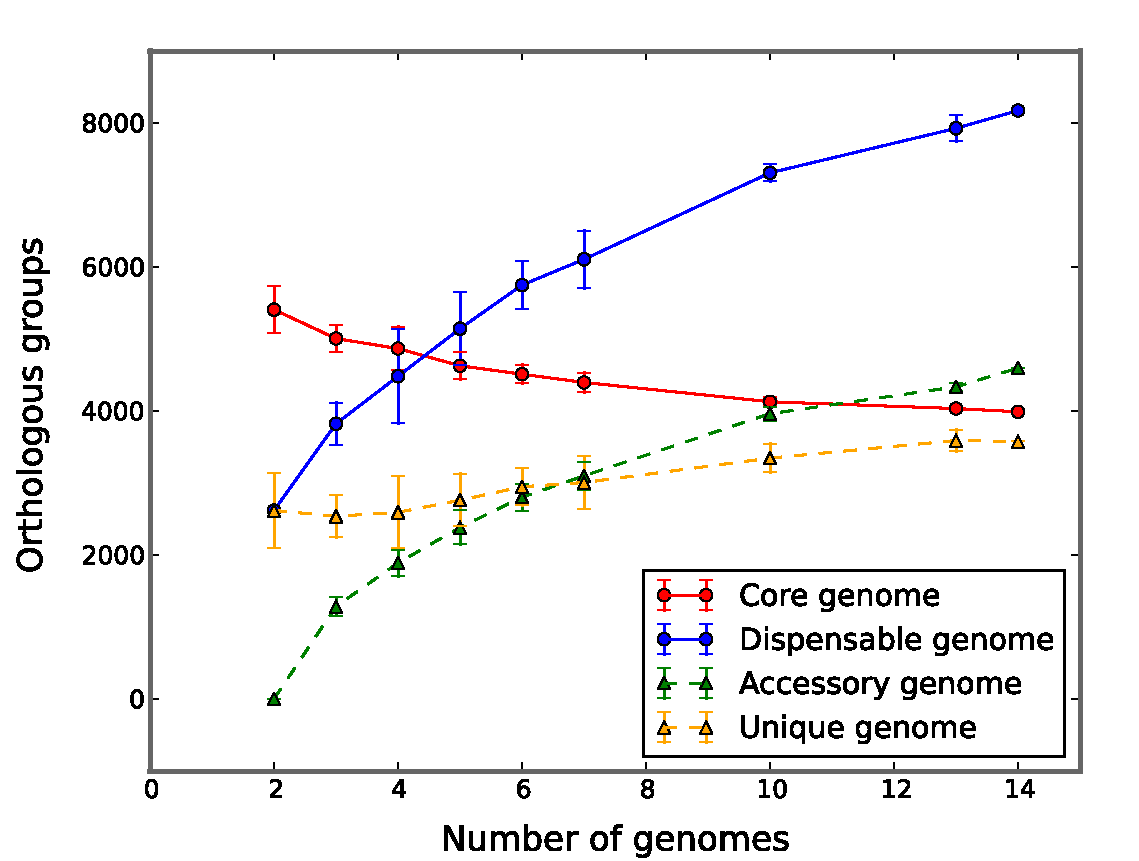
\includegraphics[width=0.8\textwidth]{figures/4/thesis_27}
	\caption{\label{fig:pangenome}\textbf{\textit{S. meliloti} pangenome permutations statistics.}\\Each point indicates the number of orthologs that are found in each pangenomic fraction. The trend lines on the median values are shown}
\end{figure}

The draft genome sequences of 10 \textit{S. meliloti} strains reported in Table \ref{tab:genomestats} were produced as described in Materials and Methods. The comparison of those 10 genomes with the complete sequences of the four strains already available at December 2011 (Rm1021, AK83, BL225C, SM11) showed that genome sizes varied from 6.69 Mbp (Rm1021) to 8.94 Mbp (5A14), with an average GC content of 61.9\%. The number of ORFs ranged from 6218 (Rm1021) to 8735 (5A14). The partial assembly of the new genomes was performed by contigs mapping with the four completely assembled genomes (Rm1021, AK83, BL225C, SM11): interestingly the newly sequenced genomes also possessed sequences belonging to the "rare" accessory plasmids such as pSINME01 and pSINME02 of strain AK83 and pSme11a and pSme11b of strain SM11. In particular all ten newly sequenced genomes contained sequences found in the accessory pSINME01 plasmid of strain AK83. Finally, 30\% of ORFs had no predicted function, while the proportion of proteins annotated by standard annotation sources ranged from 44.8\% (KEGG) to 83.3\% (Interpro). The highest annotation signal for all genomes was found, as expected, by homology with genes present in Rhizobase (86.4\%).
By comparing the 102082 ORFs found in the 14 genomes, a set of 12162/19003 orthologous groups (OGs) (using InParanoid or BBH respectively) was identified; a subset of 3989/4685 OGs was conserved across all genomes (core genome). The remaining 8173/14762 OGs were defined as members of the dispensable genome. Figure \ref{fig:pangenome} summarizes the results obtained comparing the 14 genomes of S. meliloti strains in relation to the core/dispensable genome and accessory and unique gene distribution. \textit{S. meliloti} appears to have an open pangenome, fitting the general Heaps law, $n = \kappa N\gamma$, with $\gamma$ higher than 0 \cite{tettelin2008comparative}, but has also a relatively stable core genome, accounting for slightly less than 4000 OGs. Genomic fluidity ($\phi$) is 0.32, in the range found for intra-specific polymorphism \cite{kislyuk2011genomic} and in agreement with that of other rhizobial species \cite{tian2012comparative}.

\begin{sidewaystable}[htbp]
  \tabcolsep 4pt
  \tiny
  \centering
    \begin{tabular}{rrcccccccccccccc@{}}
    \toprule
          &       & \multicolumn{14}{c}{\textbf{Strains}} \\
    \midrule
          &       & \textbf{1A42} & \textbf{5A14} & \textbf{A0641M} & \textbf{A0643DD} & \textbf{AE608H} & \textbf{AK11} & \textbf{AK75} & \textbf{C0431A} & \textbf{C0438LL} & \textbf{H1} & \textbf{Rm1021} & \textbf{AK83} & \textbf{BL225C} & \textbf{SM11} \\
    \multicolumn{1}{c}{\multirow{7}[1]{*}{\begin{sideways}\textbf{General stats}\end{sideways}}} & Length (Mb) & 7.16  & 8.94  & 7.95  & 7.35  & 7.35  & 6.84  & 6.99  & 7.09  & 7.06  & 6.92  & 6.69  & 7.14  & 6.98  & 7.5 \\
    \multicolumn{1}{c}{} & G+C content & 62.02 & 61.98 & 61.88 & 61.84 & 62    & 62.03 & 61.86 & 61.96 & 61.96 & 61.96 & 0.61  & 0.62  & 0.62  & 61.91 \\
    \multicolumn{1}{c}{} & Coding \% & 85.25 & 85.57 & 85.17 & 85.28 & 85.46 & 85.75 & 85.28 & 85.2  & 85.44 & 85.11 & 86.13 & 82.53 & 84.56 & 86.4 \\
    \multicolumn{1}{c}{} & Coding & 6106284 & 7652148 & 6774171 & 6269850 & 6279117 & 5868819 & 5963196 & 6037653 & 6035811 & 5892396 & 5763546 & 5893086 & 5901528 & 6479490 \\
    \multicolumn{1}{c}{} & ORFs  & 7374  & 8735  & 8411  & 7771  & 7197  & 6895  & 7555  & 7386  & 7242  & 6993  & 6218  & 6518  & 6359  & 7428 \\
    \multicolumn{1}{c}{} & rRNA  & 6     & 24    & 9     & 4     & 18    & 2     & 5     & 2     & 5     & 9     & 9     & 9     & 9     & 9 \\
    \multicolumn{1}{c}{} & tRNA  & 56    & 78    & 63    & 51    & 63    & 47    & 56    & 48    & 52    & 52    & 54    & 56    & 55    & 56 \\
    \multicolumn{1}{c}{\multirow{7}[0]{*}{\begin{sideways}\textbf{Annotation stats(\%) *}\end{sideways}}} & No function & 30.47 & 30.02 & 34.7  & 34.15 & 31.22 & 28.66 & 31.41 & 31.02 & 31.61 & 29.73 & 23.72 & 28.91 & 25.93 & 32.77 \\
    \multicolumn{1}{c}{} & ORFans & 3.38  & 3.57  & 3.67  & 3.35  & 1.92  & 3.16  & 3.45  & 2.4   & 3.02  & 2.89  & 1.74  & 2.75  & 0.3   & 0.7 \\
    \multicolumn{1}{c}{} & COG   & 69.53 & 69.98 & 65.3  & 65.85 & 68.78 & 71.34 & 68.59 & 68.98 & 68.39 & 70.27 & 76.28 & 71.09 & 74.07 & 67.23 \\
    \multicolumn{1}{c}{} & Interpro & 87.86 & 86.14 & 84.65 & 85.28 & 85.24 & 88.69 & 87.66 & 85.96 & 86.33 & 88.15 & 88.68 & 84.84 & 87.42 & 81.35 \\
    \multicolumn{1}{c}{} & GO    & 62.19 & 63.18 & 59.09 & 59.85 & 62.05 & 63.9  & 61.69 & 61.72 & 61.39 & 62.81 & 67.88 & 64.32 & 66.06 & 61.16 \\
    \multicolumn{1}{c}{} & KEGG  & 44.36 & 45.2  & 41.31 & 41.56 & 44.69 & 45.82 & 43.35 & 43.39 & 43.84 & 44.96 & 50.63 & 46.59 & 48.51 & 43.09 \\
    \multicolumn{1}{c}{} & Rhizobase** & 87.32 & 78.95 & 83.21 & 84    & 84.8  & 88.7  & 87.4  & 86.79 & 85.97 & 88.07 & 92.23 & 87.48 & 90.64 & 84.05 \\
    \multicolumn{1}{c}{\multirow{8}[0]{*}{\begin{sideways}\textbf{Replicon sizes (bp)}\end{sideways}}} & Chromosome & 3731100 & 4990772 & 4063405 & 3643054 & 3891677 & 3572765 & 3447294 & 3613238 & 3588400 & 3558302 & 3650000 & 3820000 & 3670000 & 3908022 \\
    \multicolumn{1}{c}{} & Chromid pSymB & 1588418 & 1878443 & 1754039 & 1593848 & 1630437 & 1565308 & 1647631 & 1558480 & 1626313 & 1603718 & 1680000 & 1680000 & 1690000 & 1632395 \\
    \multicolumn{1}{c}{} & Megaplasmid pSymA & 1396116 & 1506164 & 1457555 & 1307958 & 1285253 & 1387542 & 1518412 & 1389865 & 1313050 & 1374799 & 1350000 & 1310000 & 1610000 & 1633319 \\
    \multicolumn{1}{c}{} & pSINME01 & 209195 & 232672 & 111645 & 136588 & 125681 & 109990 & 76265 & 112338 & 94450 & 127226 &       & 260000 &       &  \\
    \multicolumn{1}{c}{} & pSINME02 &       &       &       & 11278 &       & 25905 &       &       & 7018  &       &       & 70000 &       &  \\
    \multicolumn{1}{c}{} & pSmeSM11b & 140640 & 178756 & 63273 & 122560 & 132879 & 11263 & 33722 &       & 71081 & 13413 &       &       &       & 181251 \\
    \multicolumn{1}{c}{} & pSmeSM11a & 14949 &       & 3811  & 232455 &       & 19702 &       & 14801 & 3810  &       &       &       &       & 144170 \\
    \multicolumn{1}{c}{} & Not mapped & 82306 & 155746 & 499985 & 304164 & 281255 & 151462 & 269272 & 398109 & 360652 & 245693 &       &       &       &  \\
    \bottomrule
    \end{tabular}%
  \caption{\textbf{Main features of the fourteen \textit{S. meliloti} genomes}\\
  			\textbf{*} \% on total ORFs\\
  			\textbf{**} Strain Rm1021 is excluded}
  \label{tab:genomestats}%
\end{sidewaystable}%

\subsubsection{Core and dispensable genome microevolution: replicon-based, intra-species differentiation}
\begin{figure}[!tb]
	\center
    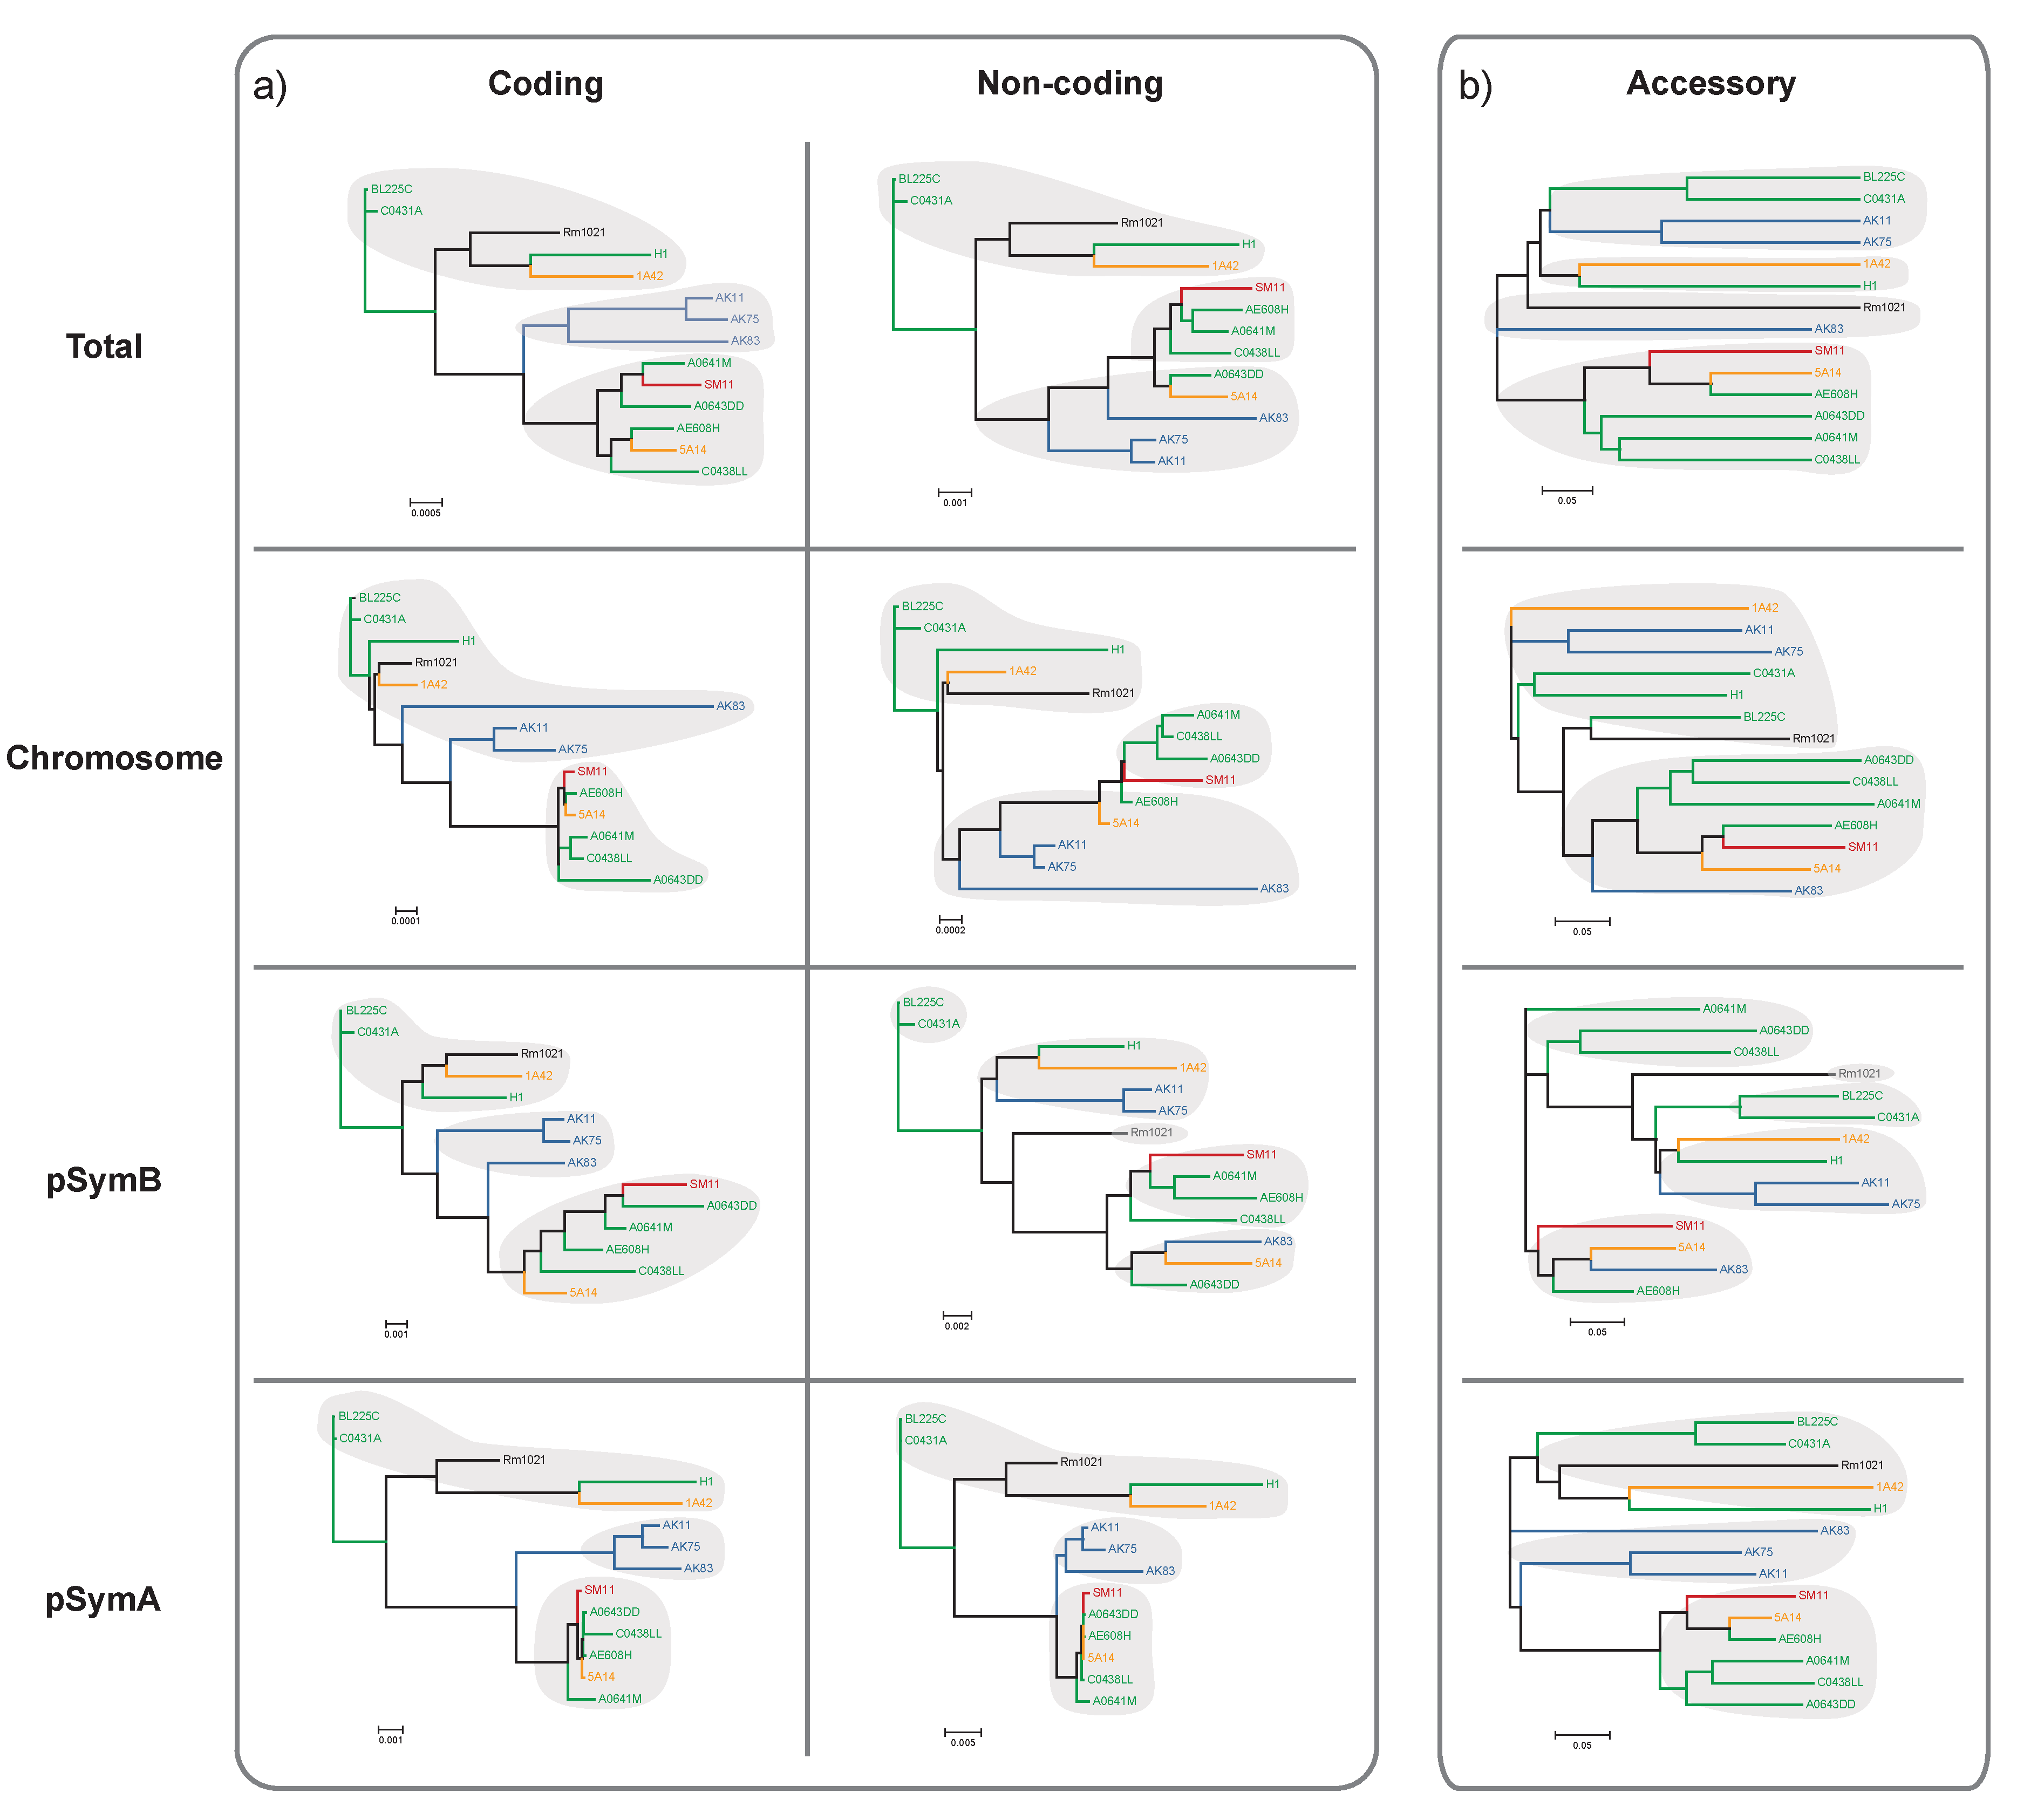
\includegraphics[width=1\textwidth]{figures/4/thesis_28}
	\caption{\label{fig:dendrogram}\textbf{Dendrograms of 14 the \textit{S. meliloti} strains based on pangenome content}\\Gray shades indicate the dendrogram’s clusters, strain names and branches are colored after the geographical origin of each strain (black: reference strain Rm1021; red: Germany; yellow: Iran; blue: Kazakhstan; green: Italy)\\
	a) Bayesian consensus dendrogram of \textit{S. meliloti} strains from core genome sequences alignments; both coding and non coding sequences dendrogram are reported\\
	b) Neighbor joining dendrograms with respect to the pattern of occurrence of 4602 accessory orthologs in the accessory genome.}
\end{figure}

Since the evolutionary dynamics in bacteria is different in the core and the dispensable genomes, we analyzed separately the genetic relationships among the 14 strains by using core genome loci and the pattern of differential occurrence of genes in the accessory genome. Moreover, for core genome, individual analyses of  the three main single replicons  and also of noncoding sequences were performed.
Concerning core genome diversity, four Bayesian dendrograms were reconstructed based on a concatenamer of nucleotide sequences of all core genome CDSs and noncoding sequences  mapped to the chromosome, pSymB and to pSymA (Figure \ref{fig:dendrogram}a). Moreover, a dendrogram with a concatenamer of nucleotide sequences of all CDS shared between the 14 S. meliloti strains, \textit{S. fredii} NGR234 and \textit{S. medicae} WSM419 was constructed, showing that S. meliloti strains, even though they are similar to \textit{S. fredii} NGR234 and \textit{S. medicae} WSM419, are well separated from these two different species. 
Additionally, to evaluate accessory genome relationships, a dendrogram from differential occurrence of accessory OGs was computed (Figure \ref{fig:dendrogram}b). In general from 2 to 5 clusters  were detected in the dendrograms of the 14 strains. The overall trees showed differential clusterizations: the coding fraction in the total tree and the coding fraction of chromid pSymB showed a 3-clusters arrangement that was also found in all the partitions of the megaplasmid pSymA; the megaplasmid shows then a similar signature, even at the accessory genome level. The Kazakhstan strains clustered  together in all the fraction of  pSymA and  in total and pSymB coding fraction in agrement with previous observations about the role of geographical isolation in \textit{S. meliloti} differentiation \cite{talebi2008diversity}. The chromosome showed a higher compactness, as expected for this more evolutionary conserved replicon, with 2 clusters for the coding and the accessory component, and 3 clusters for the non-coding component.The chromid pSymB showed the highest number of clusters, 3 for the coding component and 5 for the non-coding and the accessory components, suggesting a prominent role of this replicon for the differentiation within the \textit{S. meliloti} species.
To quantitatively evaluate the similarity between the accessory genome and core genome, Mantel's tests were carried out comparing the distance matrices obtained from core and accessory genome. Significant values for r Mantel's coefficient were found in all comparison, and the highest r value (r = 0.778) was obtained for pSymA, confirming earlier reports on the main role of pSymA on dispensable genome dynamics \cite{giuntini2005large}\cite{donini2009genome}. Moreover, distance matrices  of the three  main replicons CDSs were only partially (tough significantly) correlated  with r=0.623 (p<0.001) for pSymB-pSymA, r=0.510 for pSymA-chromosome and 0.524 (p<0.001) -for pSymB-chromosome. The same approach was used to compare trees of CDSs and surrounding noncoding regions, and, as expected, high correlation values were found r= 0.862, 0.902, 0.930 for chromosome, pSymB and pSymA, respectively, (p<0.001), suggesting a coevolution of CDS and of their noncoding flanking regions.  

\subsubsection{Evolutionary pressure on CDS: replicon-based patterns of positive selection}
\begin{figure}[!tb]
	\center
    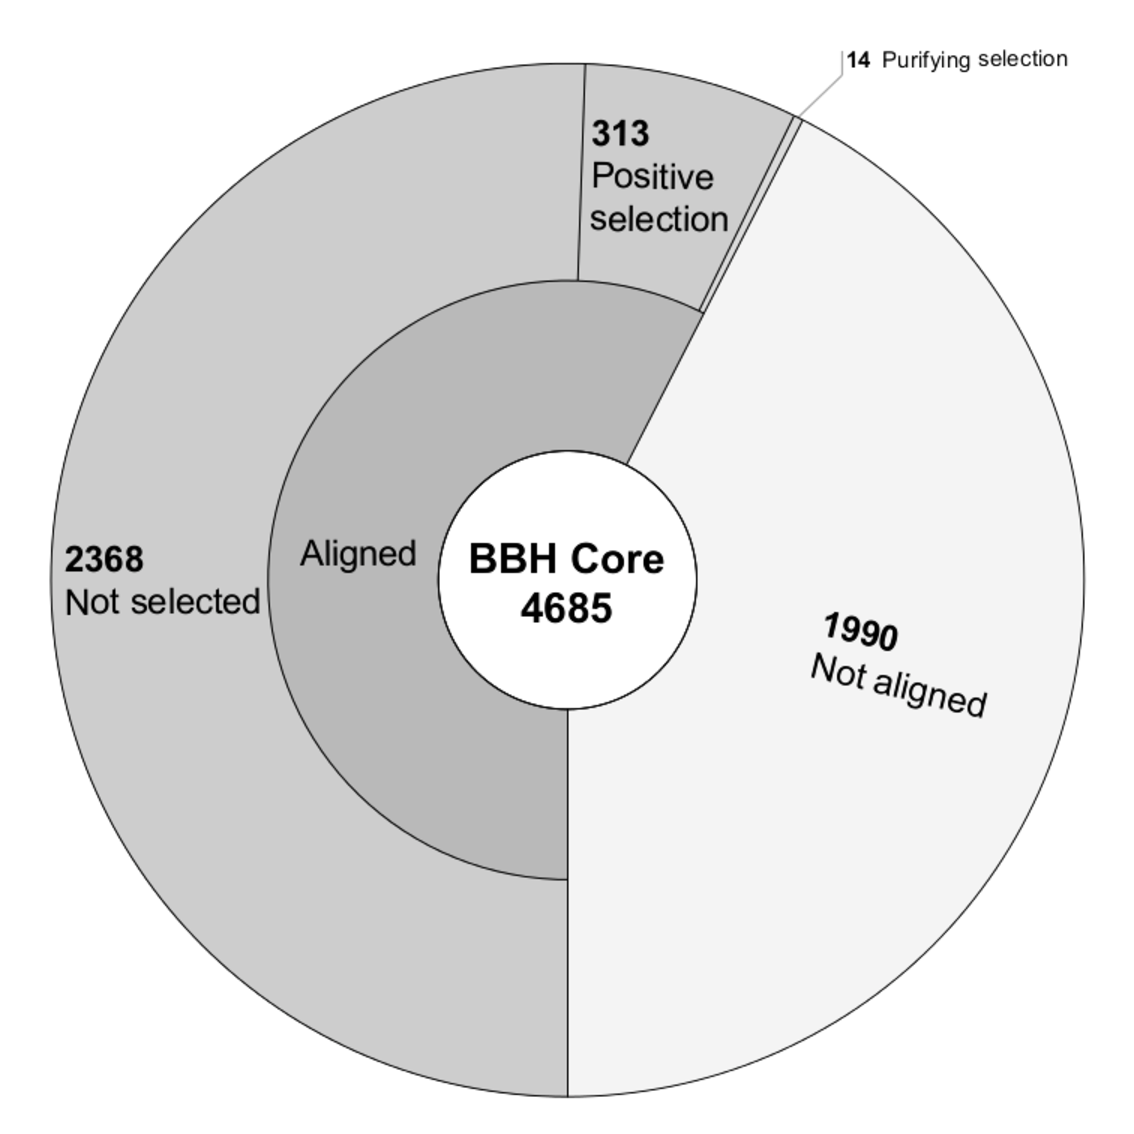
\includegraphics[width=0.66\textwidth]{figures/4/thesis_29}
	\caption{\label{fig:positive}\textbf{Krona \cite{brian12interactive} pie chart of positively selected genes from 4685 BBH-retrieved ortholog groups}}
\end{figure}

To detect whether the different evolutionary forces acting on the three main replicons (chromosome, chromid pSymB, megaplasmid pSymA) effect gene evolution through purifying and positive selection, a genome-wide scanning for genes subjected to these evolutionary forces was performed following a general computational approach previously used in several bacterial species \cite{biswas2006genomic}\cite{petersen2007genes}. Within 2695 core aligned OGs, a total of 10 OGs under purifying selection were detected, as well as 313 positively selected OGs (Figure \ref{fig:positive}). The genes under purifying selection were evenly distributed in the three main replicons and comprised the fixO1 gene involved in nitrogen fixation, as well as bacA, which encodes for one of the key factors for the establishment of an effective symbiosis \cite{glazebrook1993rhizobium}, The highest percentage (11.4\%, 150 OGs) of genes under positive selection was found for OGs located (at least in one strain) on chromid pSymB, while 5.8\% (40 OGs) were located on megaplasmid pSymA and only 4.7\% of total aligned OGs (153) were located in the chromosome (Figure \ref{fig:positivereplicons}a). This high fraction of positively selected genes may match part of the phenotypic variability observed in natural populations \cite{biondi2009metabolic}. Notably, within the positively selected genes on pSymB, we detected genes coding for putative short chain oxidoreductases, which may have roles in hydroxybutyate accumulation \cite{jacob2008mutational}, or involved in osmotolerance, as eutA \cite{jebbar2005ectoine}, or in rhizopine uptake, as mocBD \cite{rossbach1994molecular}; interestingly, the mocD gene was found to exhibit also signs of purifying selection. On pSymA, we interestingly found positively selected genes involved in Nod Factor biosynthesis and host plant preference, such as nodCHLP \cite{roche1996common}, and the gene encoding for NoeB host specific nodulation protein, the FixB electron transfer flavoprotein alpha chain, involved in nitrogen fixation and, rpoE6/rpoE (RNA polymerase ECF sigma factor). For the chromosome, genes as ntrB (nitrogen regulation protein), xylA (xylose isomerase), flgF (flagellar basal-body rod protein), ureE (urease accessory protein) were found as positively selected, which may have a role in the adaptation to stress conditions \cite{bastiat2010dual}. We computed for each COG category the ratio between selected and not selected OGs (Figure \ref{fig:positivereplicons}b) in order to evaluate if several COG categories were more represented in the positively selected genes with respect to non-selected genes. Ten COG categories showed enrichment in positive selection: interestingly, within these 10 COGs, five COG related with environmental sensing and metabolic adaptation, namely K (Transcription), M (Cell envelope biogenesis, outer membrane), N (Cell motility and secretion), G (Carbohydrate transport and metabolism) and I (Lipid metabolism), showed the highest proportional differences (> 15\%). On the opposite, three COGs, one of which containing mainly housekeeping functions (J, Translation, ribosomal structure and biogenesis; O, Post translational modification, protein turnover, chaperones and F, Nucleotide transport and metabolism), showed the lowest proportional differences (< -25\%) with the non-selected genes. It should be mentioned that indeed the chromid pSymB is particularly rich in carbohydrate transporters \cite{finan2001complete} and was supposed to play important roles in the survival of the bacterium under highly variable nutritional conditions encountered in the soil and rhizosphere. Under this view it not unexpected that an higher number of positively selected genes are resident on this replicons, suggesting that the chromid pSymB is a hot spot for adaptation in free living (non-host) highly diverse conditions, which indeed challenge bacterium’s fitness. Up to now, most of genome-wide searches for positively selected genes have been performed on pathogenic species (see for instance \cite{petersen2007genes}). These studies showed that surface proteins encoding genes are among the most relevant categories of positively selected genes, suggesting a strong role of host immune system in strain diversification. By paralleling these data, we could suppose that the evolutionary role played by host immune system variability for pathogenic bacteria is played by environmental carbohydrate scavenging by soil and rhizosphere bacteria. However, statistical evidences of positive selection should be considered with caution, since different methods may yield very different results. In a recent paper on a panel of \textit{S. meliloti} and \textit{S. medicae} strains \cite{epstein2012population}, the use of a different metrics (DTH test \cite{zeng2006statistical}) indicated that also some non essential symbiotic functions may be under positive selection, tough curiously no overlap of positively selected orthologs was found for the two species.

\begin{figure}[!t]
	\center
    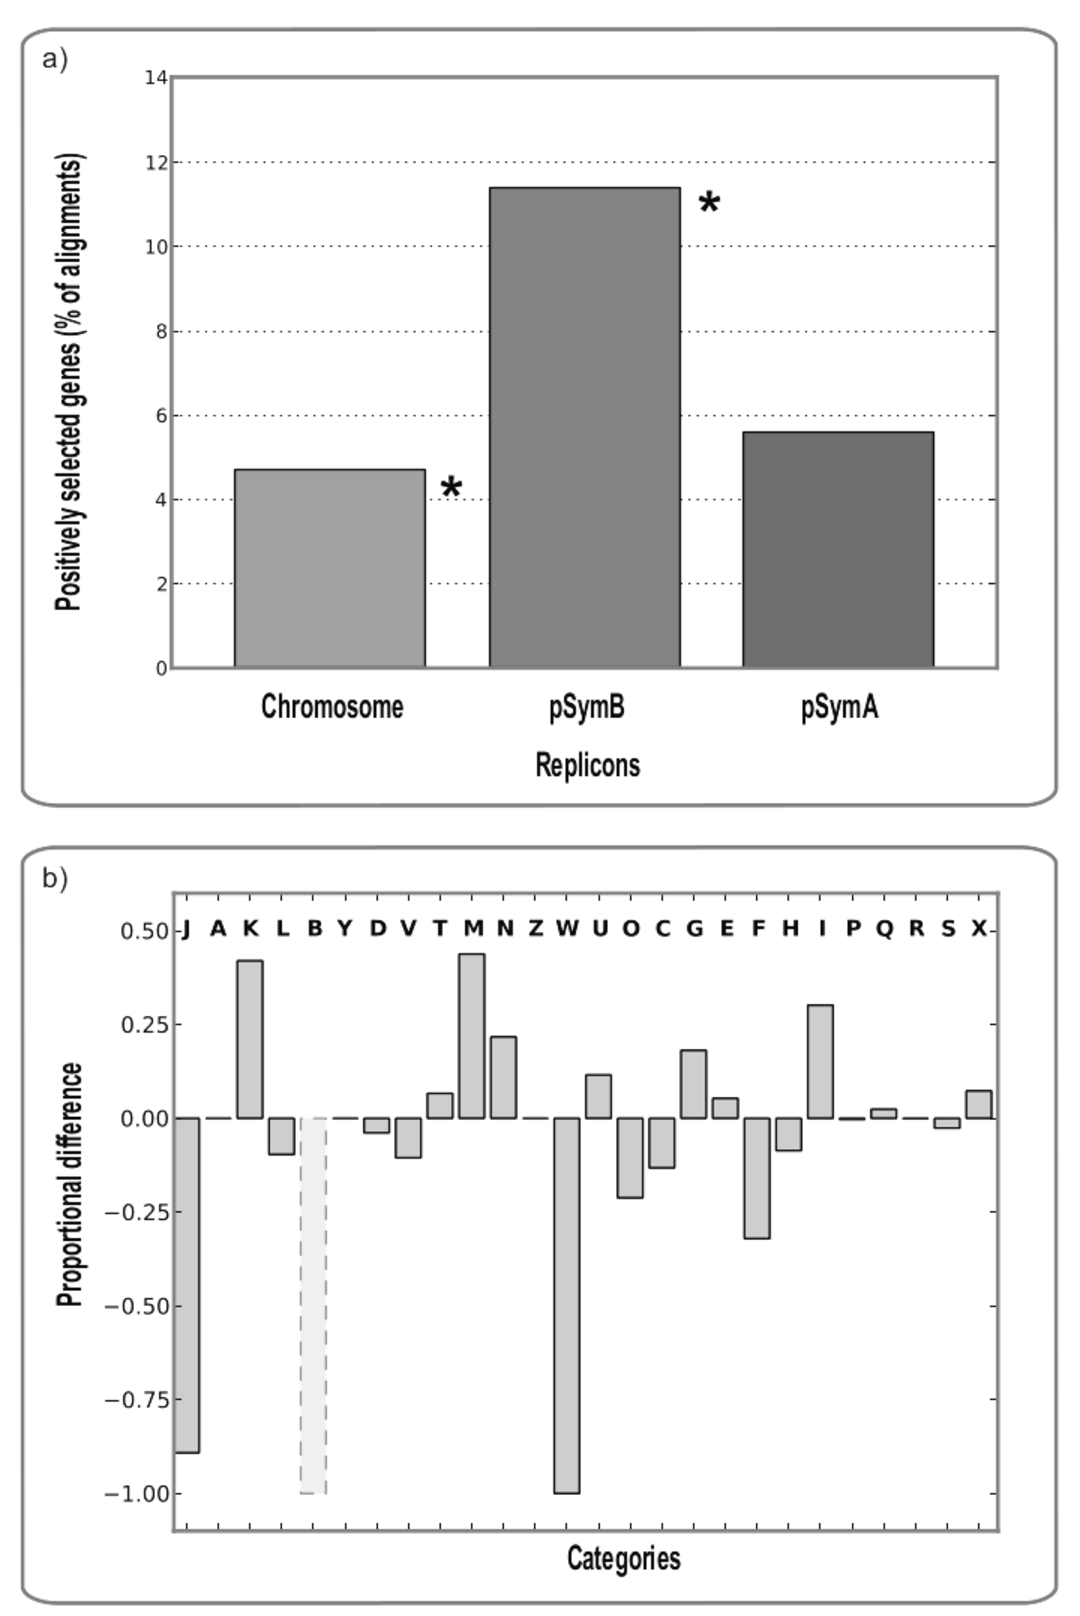
\includegraphics[width=0.66\textwidth]{figures/4/thesis_30}
	\caption{\label{fig:positivereplicons}\textbf{Detection of positively selected sites in the three main \textit{S. meliloti} replicons}\\
	a) The proportion of positively selected sites detected with respect to the total number of genes present is reported. Asterisks indicate significant enrichment (P<0.003, 3 standard deviations) of positively selected genes\\
	b) Difference between relative proportions of each COG category between selected and non selected core genes. All differences except B are significant}
\end{figure}

\subsubsection{Taxonomic distribution: chromid genes are widespread in distant taxa}
\begin{figure}[!t]
	\center
    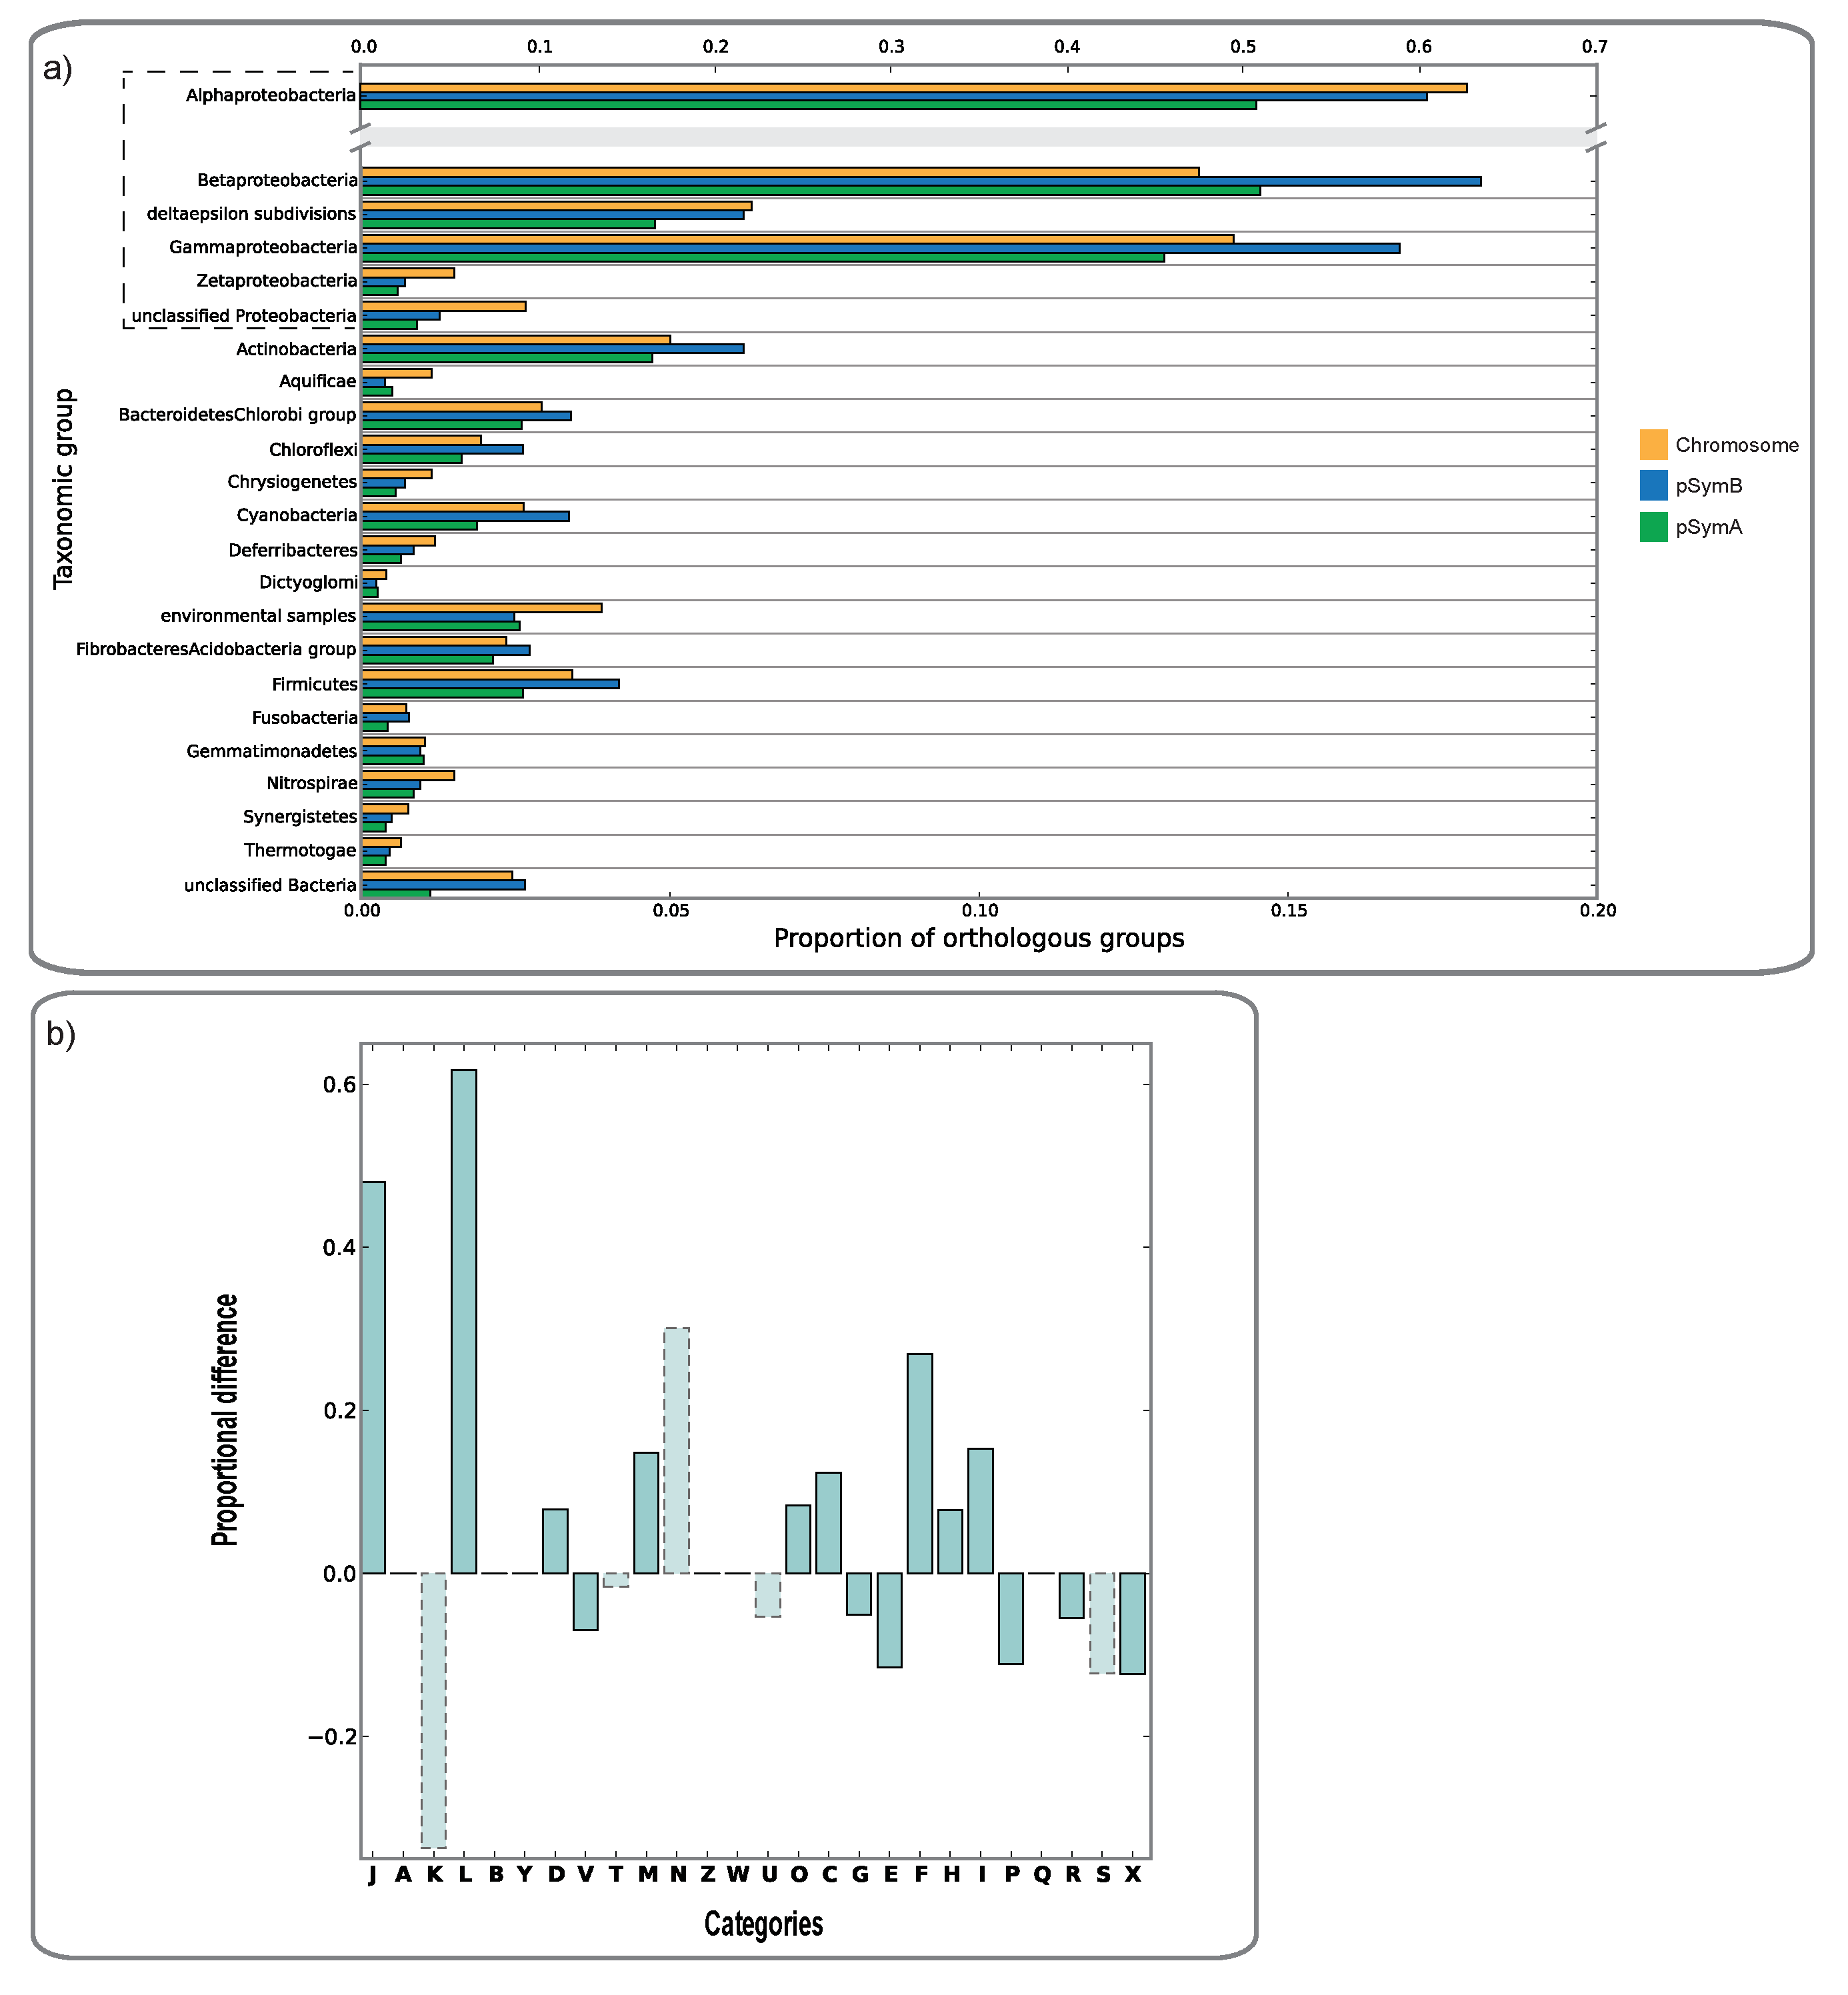
\includegraphics[width=0.9\textwidth]{figures/4/thesis_31}
	\caption{\label{fig:taxa}\textbf{Taxonomic distribution of the \textit{S. meliloti} pangenome}\\
	a) Taxonomic distribution of the OGs mapped to each replicon: for each taxonomic group, the proportion of the orthologs for each replicon having a significant hit is reported\\
	b) Difference between relative proportions of each COG category between proteobacterial hits and non-proteobacterial hits. Solid histograms mark categories with significant differences}
\end{figure}

To infer the phylogenetic origin of dispensable genome and its potential differences with respect to the phylogenetic relationships of the core genome, a homology analysis on taxonomic partitions of the nr database \cite{pini2011plant} was carried out in order to define the bacterial (and proteobacterial) phylogenetic groups to which each replicon shows the highest similarity (Figure \ref{fig:taxa}). When analyzing the orthologs with respect to their position on the three main replicons (Chromosome, pSymB and pSymA, Figure \ref{fig:taxa}a), several bacterial classes, notably \textit{Betaproteobacteria} and \textit{Gammaproteobacteria} had the highest number of matches for orthologs harbored by pSymB, while orthologs located on the chromosome and on pSymA had a (similar) lower proportion. This evidence may suggest a wider scenario for chromids evolution, which may have originated by (very ancient) gene transfer events by distant relatives and then contributed in the emergence of new taxa (e.g. genera) \cite{harrison2010introducing}. However, analyses on a large-scale dataset are needed to evaluate the taxonomic distribution of chromid-harbored genes in several genera. 
Finally, to provide functional insights over the orthologs that \textit{S. meliloti} shares with proteobacterial and non-proteobacterial taxa, the differences between hits on non-proteobacterial and proteobacterial taxa were computed for each COG category. Results of the analysis are shown in Figure \ref{fig:taxa}b. Interestingly, positive values of proportional differences were obtained for several COGs involved in housekeeping functions (as J, L, D, M, O, C, F, H, I), indicating that orthologs for these functions are significantly shared with also non-proteobacterial taxa. Conversely, COGs coding for "accessory" functions, as defense mechanisms (V), carbohydrate and aminoacid metabolism (G and E), secondary metabolites (P) are more represented in hits on proteobacterial taxa than in non-proteobacterial taxa.

\subsubsection{Structural evolution through rearrangements on a shared backbone}
\begin{figure}[!t]
	\center
    \includegraphics[width=1\textwidth]{figures/4/thesis_32}
	\caption{\label{fig:structure}\textbf{Structural alignments of the 14 \textit{S. meliloti} genomes}\\
	Alignment between genomes are reported, following the order of the overall Bayesian dendrogram (Figure \ref{fig:dendrogram}), the presence of core, accessory and unique contiguous regions of orthologs whose length is over 10 kbp is reported}
\end{figure}

To infer potential structural features (uneven or even distribution along the replicons) of the dispensable genome in the 14 strains, the 10 draft genomes were assembled using CONTIGuator \cite{galardini2011contiguator}, and the resulted reconstructed putative replicons were aligned (see Materials and  methods) to the complete genomes of AK83, BL225C, Rm1021 and SM11 strains (Figure \ref{fig:structure}). Interestingly, the dendrogram of genetic relationships between strains was well mirrored by structural features of the same strains. It is worth notice that, in fact, the three main clusters present in the dendrogram (containing Rm1021, SM11 and AK83, respectively), correspond to the presence of large inversions. Another interesting feature is the evidence that the dispensable genome and especially unique genes fractions are mainly distributed in clusters (blue and green zones, respectively). In particular pSymA contained, as expected, a higher proportion of accessory and unique contiguous blocks, while pSymB and the chromosome contained a higher proportion of core contiguous blocks, in agreement with earlier reports \cite{giuntini2005large}\cite{galardini2011exploring}. Particularly interesting is also the abundance of unique gene clusters in pSymA (roughly 10\% of the total, against the 5\% proportion of the chromosome and the chromid), compared to the other large replicons (Figure \ref{fig:structure2}); in the two smaller plasmids a significant higher fraction of dispensable contiguous block is present, as expected  in such small accessory plasmids.
\begin{figure}[!tb]
	\center
    \includegraphics[width=0.77\textwidth]{figures/4/thesis_33}
	\caption{\label{fig:structure2}\textbf{Structural analysis of the 14 \textit{S. meliloti} genomes}\\
	Proportion of contiguous regions for each pangenomic category in each replicon}
\end{figure}
The arrangement of the unique gene fraction in blocks on \textit{S. meliloti} genomes is particularly relevant, since unique genes are used as models for inferring de novo gene evolution. Unique gene evolution models hypothesize that transcriptional and translational events in noncoding regions or sporadic phage integrations are fixed and, after passing the natural selection filter, lead to the emergence of unique (novel) genes \cite{yomtovian2010composition}\cite{carvunis2012proto}. In this perspective, the slightly higher abundance of unique and dispensable genes found on pSymA makes sense with either a higher proportion of mobile genetic elements there residents \cite{biondi2011spread} and with the lower percentage of protein-coding DNA (and consequently higher intergenic regions length) in pSymA, with respect to the chromosome and to pSymB \cite{galardini2011exploring}.
\begin{figure}[!tb]
	\center
    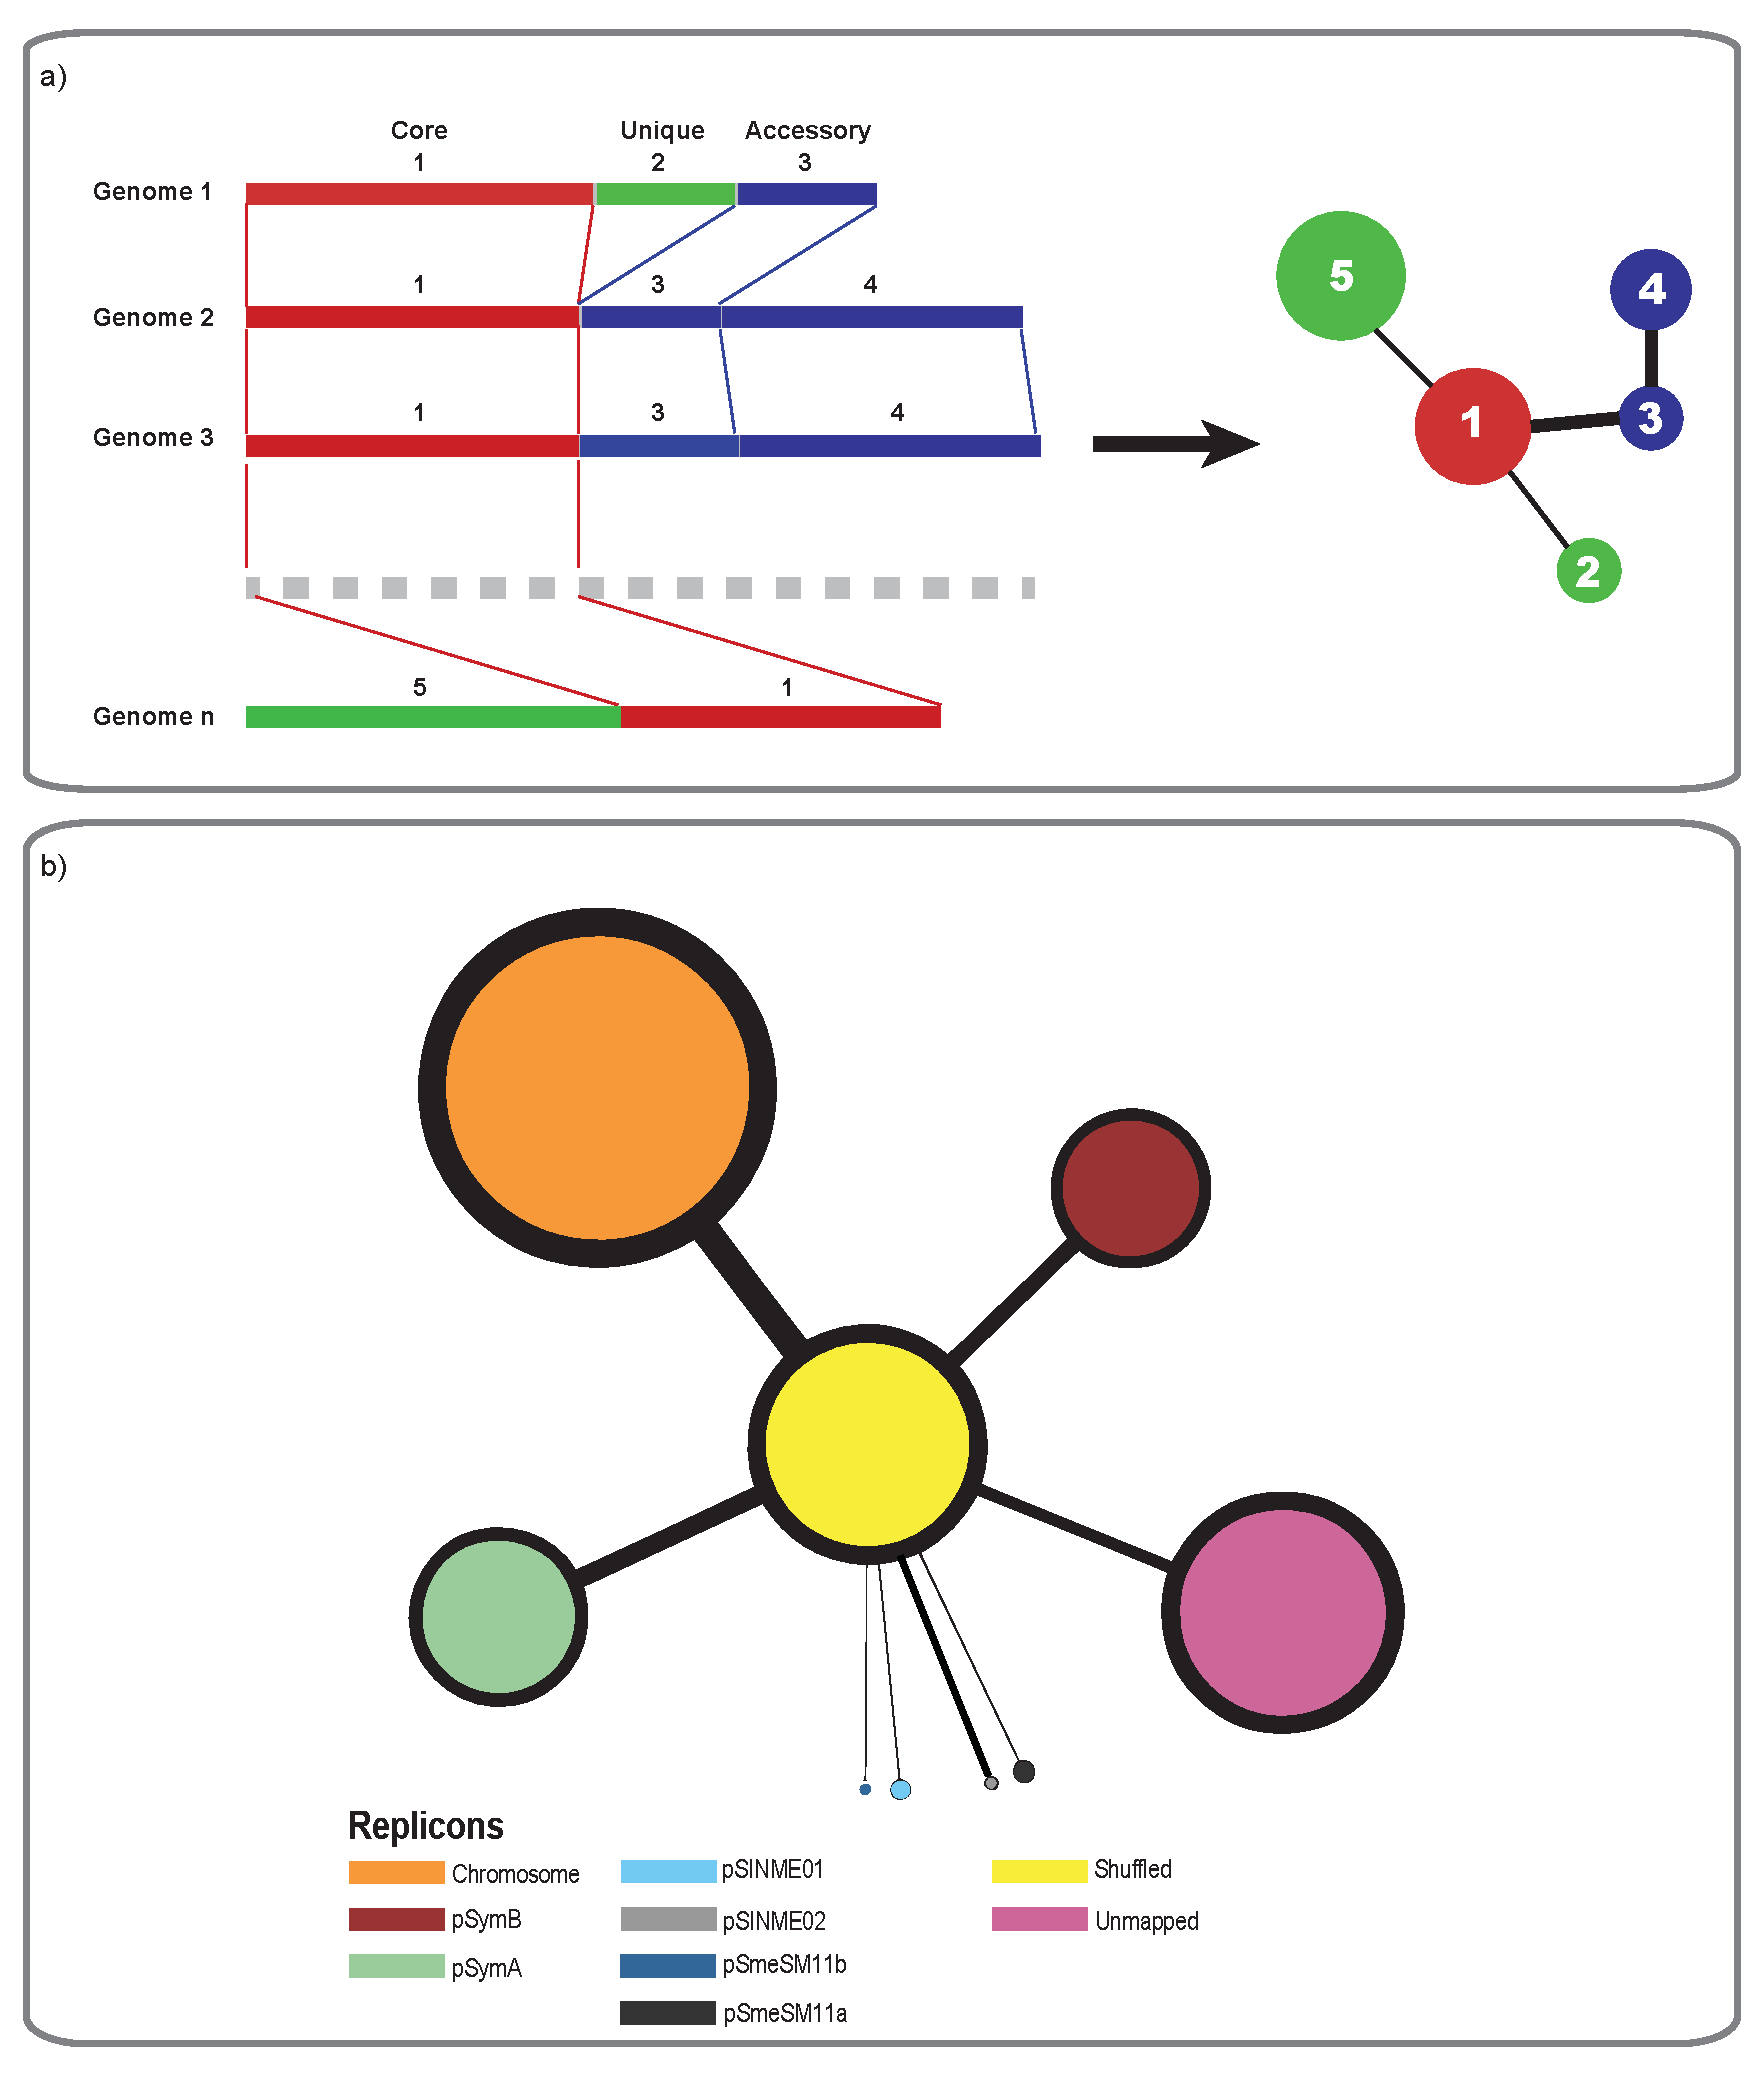
\includegraphics[width=0.77\textwidth]{figures/4/thesis_34}
	\caption{\label{fig:network}\textbf{Proximity network construction and statistics}\\
	a) Explanatory proximity network construction details\\
	b) Block model simplified version of the proximity network, obtained dividing the nodes according to their replicon of origin; nodes and edges sizes are proportional to the number of orthologs and number of links observed, respectively}
\end{figure}
To understand how the genomic structure evolves, a deeper structural analysis was then performed through the exploitation of the DNA proximity network; the network has been constructed so that each node represents a nucleotide region present in one or more genomes, while the edges represent the proximity of each region to the others on one or more genomes, the weight of the edge being proportional to the number of times each link is observed in the whole pangenome (Figure \ref{fig:network}a). A total number of 24518 nodes (with an average size of 894 bp) and 36781 edges were added to the network: each node was assigned to its replicon of origin, “Shuffled” (if the node was mapped to more than one replicon in the pangenome) or “UnMapped” (if the node wasn’t assigned to any replicon). A simpler block-model network was then constructed using the replicon information, the nodes size proportional to the bases mapped and the edges proportional to the number of links between each replicon (Figure \ref{fig:network}b): as expected the largest node is that representing the chromosome, with 6.58 Mb mapped in the whole pangenome, followed by the Shuffled and UnMapped nodes (4.34 and 4.38 Mb respectively); interestingly, the megaplasmid pSymA showed a higher number of bases than the chromid (3.19 and 2.83 Mb respectively), a feature that can be explained by the higher number of accessory regions mapping to this replicon, which in fact leads to a megaplasmid which is larger than the chromid in pangenomic terms.

\begin{sidewaystable}[htbp]
  \centering
  \tiny
    \begin{tabular}{rrrrrrrrrrr}
    \toprule
          & \multicolumn{10}{c}{\textbf{DNA Proximity Network cluster}} \\
    \midrule
          & \multicolumn{1}{c}{All} & \multicolumn{1}{c}{Mapped} & \multicolumn{1}{c}{Shuffled} & \multicolumn{1}{c}{Chromosome} & \multicolumn{1}{c}{pSymB} & \multicolumn{1}{c}{pSymA} & \multicolumn{1}{c}{pSINME01} & \multicolumn{1}{c}{pSmeSM11b} & \multicolumn{1}{c}{pSINME02} & \multicolumn{1}{c}{pSmeSM11a} \\
    \textbf{Average Degree*} & 3.00  & 2.91  & 2.63  & 2.98  & 2.88  & 2.77  & 2.43  & 2.79  & N/A   & 2.42 \\
    \textbf{Std-dev Degree*} & 1.00  & 0.97  & 0.81  & 1.00  & 0.97  & 0.89  & 0.73  & 0.89  & 0.00  & 0.72 \\
    \textbf{Replicon Assortativity} & 0.67  & 1.00  & N/A & N/A & N/A & N/A & N/A & N/A & N/A & N/A \\
    \textbf{Major component Weighted size} & 1.00  & 0.21  & 0.19  & 0.43  & 0.17  & 0.29  & 0.13  & 0.56  & 0.04  & 0.13 \\
    \textbf{Boundary weighted size**} & N/A & 0.34  & N/A & 0.27  & 0.34  & 0.44  & 0.94  & 0.68  & 1.00  & 0.70 \\
    \bottomrule
    \end{tabular}%
  \caption{\textbf{DNA proximity network statistics}\\
  \textbf{*} Considering nodes with degree > 1\\
  \textbf{**} Nodes having at least a link to the shuffled cluster}
  \label{tab:proximity}%
\end{sidewaystable}%

A series of network statistics were computed for the overall network (“All”), the nucleotidic regions univocally mapped to one replicon (“Mapped”), the shuffled regions (“Shuffled”) and the single replicons (Table \ref{tab:proximity}): the overall network had the highest average node degree (\textasciitilde 3), meaning that each node is connected to three other nodes on average, resulting in a relatively non-conserved structure in the whole pangenome; when considering the replicon assortativity (a measure of how much each node tends to be closer to a node coming from the same replicon), the highest value is found for the “Mapped” component, meaning that when the shuffled nodes are removed from the proximity network, the single replicons have no links connecting each other, thus suggesting indeed the presence of a conserved core structure for each replicon. This finding was further confirmed looking at the size of the major connected component (that is, the largest subgraph in which each node can be reached from any other node): only \textasciitilde 21\% of the “Mapped” component was linked in a single cluster; when considering the larger replicons, the chromosome was found to have the larger fraction of its content present in a single cluster (\textasciitilde 43\%), while lower values for the other two replicons, meaning that the chromosome structure is evolutionary more conserved, with nearly half of its nucleotidic content with a conserved structure. As expected, the opposite trend was observed when looking at the fraction of genes of each cluster that were present in the “boundary” to the shuffled component (which are the nodes having an edge to a node in the shuffled component), ranging from \textasciitilde 27\% (chromosome) to 100\% (pSINME02), with the megaplasmid having the highest proportion of nodes in boundary among the larger replicons (\textasciitilde 44\%), meaning that the megaplasmid experienced a higher number of rearrangements than the other replicons. This observation is confirmed when looking at the number of putative transposases encoded in each replicon, with the megaplasmid pSymA harboring almost three times the transposases found in the chromosome and in the chromid, a feature that could explain the higher fluidity of this replicon.
\begin{table}[htbp]
  \centering
    \begin{tabular}{rrrrr}
    \toprule
          & \textbf{All} & \textbf{Chromosome} & \textbf{pSymB} & \textbf{pSymA} \\
    \midrule
    \textbf{Number of chains} & 1035  & 349   & 118   & 60 \\
    \textbf{Total length (Mb)} & 2.68  & 2.03  & 0.51  & 0.27 \\
    \textbf{Length proportion*} & N/A   & 0.54  & 0.31  & 0.18 \\
    \textbf{Average length (bp)} & 5391.9 & 5819.7 & 4342.4 & 4502.2 \\
    \textbf{Std-size size (bp)} & 6561.6 & 6281.8 & 6257.8 & 5522.5 \\
    \textbf{Average degree**} & 2.00  & 2.00  & 2.00  & 2.00 \\
    \textbf{Std-dev degree**} & 0.00  & 0.00  & 0.00  & 0.00 \\
    \bottomrule
    \end{tabular}%
    \caption{\textbf{DNA backbones statistics}\\
    			\textbf{*} Replicon size is the average replicon length in the four complete \textit{S. meliloti} genomes\\
			\textbf{**} Considering nodes with degree > 1}
	\label{tab:chains}%
\end{table}%
To inspect if there was a conserved structural backbone in the pangenome, the overall network was divided using a filter on the links weight, that are proportional to the number of times two nucleotide regions are seen as adjacent in the whole pangenome (Figure \ref{fig:network}a), leading to the definition of “DNA backbones”, which are the largest conserved genomic structures in the \textit{S. meliloti} pangenome; both the overall backbones and the replicon specific backbones were computed (Table \ref{tab:chains}).  For all the three categories used, only linear backbones were found (degree=2), with a similar average length of roughly 5'000 bp, meaning that the underlying mechanisms of formation and evolution of these backbones may be similar in the three replicons; on the other hand, the proportion of replicons conserved in a backbone varies between each replicon: roughly half of the chromosome is conserved and contained in a single backbone, one third of the chromid pSymB is conserved, while just 18\% of the megaplasmid pSymA is conserved; thus, even though the mechanisms of structural evolution are similar in each replicon, the extent of the structural variability is different.

\subsubsection{An evolutionary scenario for multipartite bacterial genomes}
\begin{figure}[!tb]
	\center
    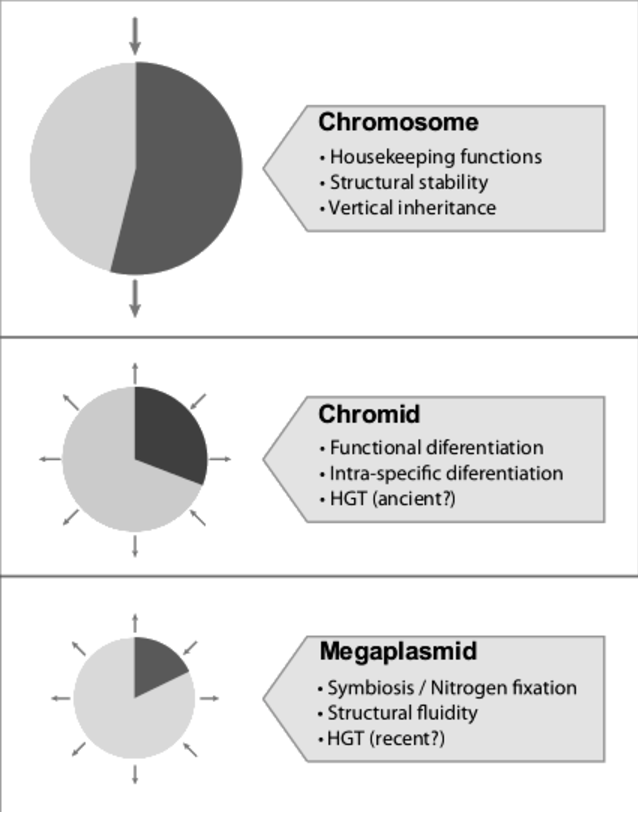
\includegraphics[width=0.6\textwidth]{figures/4/thesis_35}
	\caption{\label{fig:replicons}\textbf{Tasks and evolutionary differences of replicons in \textit{S. meliloti}}\\
	Pie charts indicate the proportion of each replicon that is present in the DNA backbones. The arrows indicate the transmission mechanism: vertical inheritance (two arrows) or HGT (radial arrows)}
\end{figure}

Bacterial genomes are classically described by the “\textit{E. coli} rules”, in which the genome is composed by one chromosome, plus additional plasmids which often carry non-essential functions \cite{krawiec1990organization}. However, this approximation fails to describe several bacterial species, for which large additional replicons are present as secondary chromosomes, megaplasmids, etc. Recently, the term “chromid” has been proposed \cite{harrison2010introducing} to describe large replicons which contain plasmid-type replication systems but also essential genes for growth and survival. 
Here the analysis of 14 \textit{S. meliloti} multipartite genomes allowed us to show that each replicon behave as partially independent evolutionary unit, suggesting that the multi-replicon structure in some bacterial species may be functional to the physical separation of different functions but also of different evolutionary pressures. This is the case of \textit{S. meliloti} which exploits multiple ecological niches (soil, rhizosphere, root nodule, plant endosphere etc. \cite{pini2012exploring}), In particular the chromid pSymB behave as an independent evolutionary unit, and our data suggest that the biological and evolutionary meaning of chromids is larger than previously hypothesized, playing a considerable role at the intraspecific level, in addition to genera differentiation \cite{harrison2010introducing}. Indeed chromids could also have a role in species differentiation as genomic elements for adaptation through individual genes evolution, while the plasmids and megaplasmids are more prone to structural evolution (e.g. via horizontal gene transfer). 
The overall evolutionary scenario of the three main S. meliloti replicons could be approximated as in Figure \ref{fig:replicons}. The chromosome contains most of the housekeeping functions and originated mainly by vertical descent from \textit{S. meliloti} phylogenetic relatives. The chromid pSymB indeed is mainly vertically transmitted in the genus Sinorhizobium \cite{harrison2010introducing} \cite{bailly2011population}, but it also acquired genes from distant relatives by primordial horizontal gene transfer events. Functions of pSymB are mainly related to exploitation of environment and evolution takes place through positive selection of genes involved in environmental exploitation. Finally, the megaplasmid pSymA, as alien element (its GC content is significantly different from those of chromosome and of chromid \cite{galibert2001composite}) is the replicon devoted to the introduction of genomic novelties (as new genes coming by horizontal gene transfer). It is worth to remember that the most relevant bioprocess of rhizobia (symbiotic nitrogen fixation) is indeed linked to this last replicons, and that functional diversification via purifying selection seems to act also on a number of symbiotic-related genes; moreover, unlike the other replicons, both core and accessory fractions show a similar pattern, indicating similar evolutionary patterns for the conserved and variable fractions in this replicon. Interestingly, at the structural level, the network analysis highlighted the presence of stable core structures in each replicons, the chromosome having the largest conserved network, followed by the pSymB chromid and finally by the pSymA megaplasmid, which was confirmed as a hot spot for structural rearrangements.
In conclusion this study demonstrates that the evolution of the \textit{S. meliloti} pangenome shows two opposite behaviors: a strongly conserved genome that evolves by positive selection on genes related to survival in complex environments, and an highly variable fraction that most likely contributes to structural fluidity and the emerging of new functions. The conserved genome signature is replicon-specific, while for the variable part the signature is more strain-specific. It is not clear yet if this model is applicable to other multipartite bacterial genomes, which contains both chromids and plasmids and may have different ecological features (e.g. Brucella, Variovorax, Vibrio, etc. for a list of genera see \cite{harrison2010introducing}). However future population genomics analyses on other species with these features will help elucidating the evolutionary role of multipartite genomes in bacteria.


%%-----------
%% Backmatter
%%-----------
\backmatter
\chaptermark{Bibliography}
\renewcommand{\sectionmark}[1]{\markright{#1}}
\bibliographystyle{unsrt}                           %Use alpha codes for references
\sectionmark{Bibliography}
\addcontentsline{toc}{chapter}{Bibliography}        %Force addition of Bibliography to TOC    
\bibliography{References}

\mainmatter
\part{Conclusions}
%%%%%%%%%%%%%%%%%%%%%%%%%%%%%%%%%%%%%%%%%%%%%%
\logvartrue
\chapter{Conclusions}
%%%%%%%%%%%%%%%%%%%%%%%%%%%%%%%%%%%%%%%%%%%%%%

The awareness about the importance of the microbial world for the higher organisms and ultimately for the human race has grown in the last decade, together with the emergence of the genomics and comparative genomics sciences. The challenges posed by a growing world population and the need for a more efficient agriculture with less waste of energy and land need to be addressed using also the vast resources that can be extracted from natural bacterial populations; the nitrogen fixation process of the \textit{Sinorhizobium} - \textit{Medicago} symbiosis it's an excellent example of a natural process that would allow a more productive and efficient agriculture, process which can be optimized through the application of a comparative genomics approach (such as gene mining).

In the first part of this thesis the development of two computational tools needed to help the comparative genomics analysis is described: the need to extract the maximum amount of information from complex draft genomes is matched by CONTIGuator, while the need to give genetic explanations to phenotypes in an automatic fashion is matched by DuctApe. Both softwares have been developed to be applied to similar problems in different species than \textit{S. meliloti} and to be widely adapted by the scientific community through a focus on usability and a clear set of results.

In the second part of the thesis the presence of a common genetic repertoire for the association of \textit{Alphaproteobacteria} with plants has been tested through a comparative genomics on a large and heterogenuos set of genomes: indeed species that are associated with plants tend to have a larger genome, putatively harboring genetic elements needed for the establishment of a successful association, either through endophytism or symbiosis: the broad range of association mechanisms lead to the impossibility to find a large repertoire of shared genetic elements for endophytism, while the genes that are most likely needed for the symbiotic process are indeed more and more defined, including for instance nodulating genes; from this analysis we can conclude that the plant symbiosis phenotype has a conserved gene repertoire inside \textit{Alphaproteobacteria}.

In the last part of the thesis, two comparative genomics studies on \textit{Sinorhizobium meliloti} have been carried on to understand if the variability in the plant growth promotion phenotype was mirrored by a variability in the genetic elements related to the symbiotic process and to understand the evolution and functional features of the peculiar genomic structure in this species. Indeed, both the presence/absence pattern of symbiotic genes and regulatory elements could be related to the observed phenotypic differences, leading to the definition of a large accessory gene set that could be furtherly tested in genetic engineering experiments towards the creation of new \textit{S. meliloti} strains. The three replicons that compose the genome of this species have also been characterized from a functional and evolutionary point of view, showing that the pSymB chromid has an important role in intra-specific differentiation and functional evolution through positive selection, while the pSymA megaplasmid has an important role in structural evolution and in the emergence of new functions.

Even though the genomics era has posed many new challenges, especially to computational biologists, the creation and application of the new analysis methods of the comparative genomics has proven to be able to help in the definition of the most probable elements that can explain functional and evolutionary differences found in the vast reservoir of diversity that is the bacterial community, a rich and promising field that needs to be studied for a better understanding of the bacterial world and its economical, agricultural and environmental impact on human life.									% Conclusions									

\mainmatter
\part{Appendices}
\appendix
\logvartrue
\chapter{Other applications of the computational tools}
\label{sec:appendix1}

\section{Enly: improving draft genomes through reads recycling}
The reconstruction of the complete genome sequence of an organism is a key point for comparative, functional and evolutionary genomics. Nevertheless, overcoming the problems encountered while completing the sequence of an entire genome is still highly demanding in terms of time and resources.
We have developed a tool (named Enly) based on the iterative mapping of sequence reads at contig edges, capable to extend the genomic contigs deriving from high-throughput 454 sequencing and Newbler assembler. We tested Enly performances in improving the assemblies of bacterial genomes sequenced by 454 pyrosequencing platform and it allowed the automated closure of about 10\% of the gaps for each of the bacterial draft genomes.
In this work we present Enly, a software allowing the extension of draft genomes contigs resulting from de novo assembly and thus being helpful during genomes finishing procedures. Enly is particularly suited to be used with long (length > 200nt) reads and with assemblers that trim contigs ends. Enly and its related documentation can be downloaded at \href{http://enly.sf.net}{http://enly.sf.net}\footnote{Marco Fondi, Valerio Orlandini, Giorgio Corti, Marco Severgnini, \textbf{Marco Galardini}, Alessandro Pietrelli, Fabio Fuligni, Michele Iacono, Ermanno Rizzi, Gianluca De Bellis and Renato Fani}.

\subsection{Introduction}
The advent of the so-called next-generation-sequencing (NGS) platforms has allowed the scientific community to approach the genome sequencing of a huge number of organisms, species and strains at reasonable costs. Indeed, determining the entire genome sequence of an organism is one of the key steps in elucidating the details of its biology, and it is also propaedeutic for a plethora of additional analyses (such as structural genomics, transcriptomics, SNPs detection) that require a complete genome sequence or, at least, a good quality draft assembly. Hence, sequence assembly is the first challenge encountered in a typical computational genomics pipeline and involves the merging and the ordering of shorter sequence fragments (reads) with the aim to get as close as possible to the original larger sequence (genome). However, many issues regarding the computational assembly of large-scale sequencing data have remained unsolved \cite{scheibye2009sequence} and, actually, the number of draft genomes in databases greatly overtakes the number of completely sequenced (closed) ones (\href{www.genomesonline.org}{www.genomesonline.org}). The output of a de novo assembly is typically a draft genome, consisting of a set of contigs (i.e. contiguous sequence fragments) that may be ordered and oriented into scaffold sequences, with gaps between them, representing regions of uncertainty \cite{earl2011assemblathon}. This may be due to several causes, including the presence of repetitive fragments along the genome and/or the absence of enough reads to produce a reliable assembly, according to the de novo assembler parameters. Approaching gaps closure in genomes (even bacterial ones) is a time-consuming and not easily automated effort, often involving the setup and the execution of a series of PCR reactions \cite{galardini2011contiguator}. Thus, pushing towards the limits of the in-silico sequence reconstruction is desirable in order to reduce the amount of laboratory work to be done after the completion of the bioinformatic procedures. Some traditional assemblers like Newbler (454 Sequencing, Roche Diagnostics, Indianapolis, IN, USA) usually perform a trimming of the contig edges depending on the quality of the supporting reads. This conservative procedure, however, may result in a loss of information, discarding many correct bases characterized by a sub-optimal quality. To overcome these limitations, we have developed a tool called Enly that allows increasing the length of the contigs deriving from Newbler assemblies and the closure of some of the gaps commonly present in the draft genome.

\subsection{Results and discussion}
\begin{figure}[!tb]
	\center
    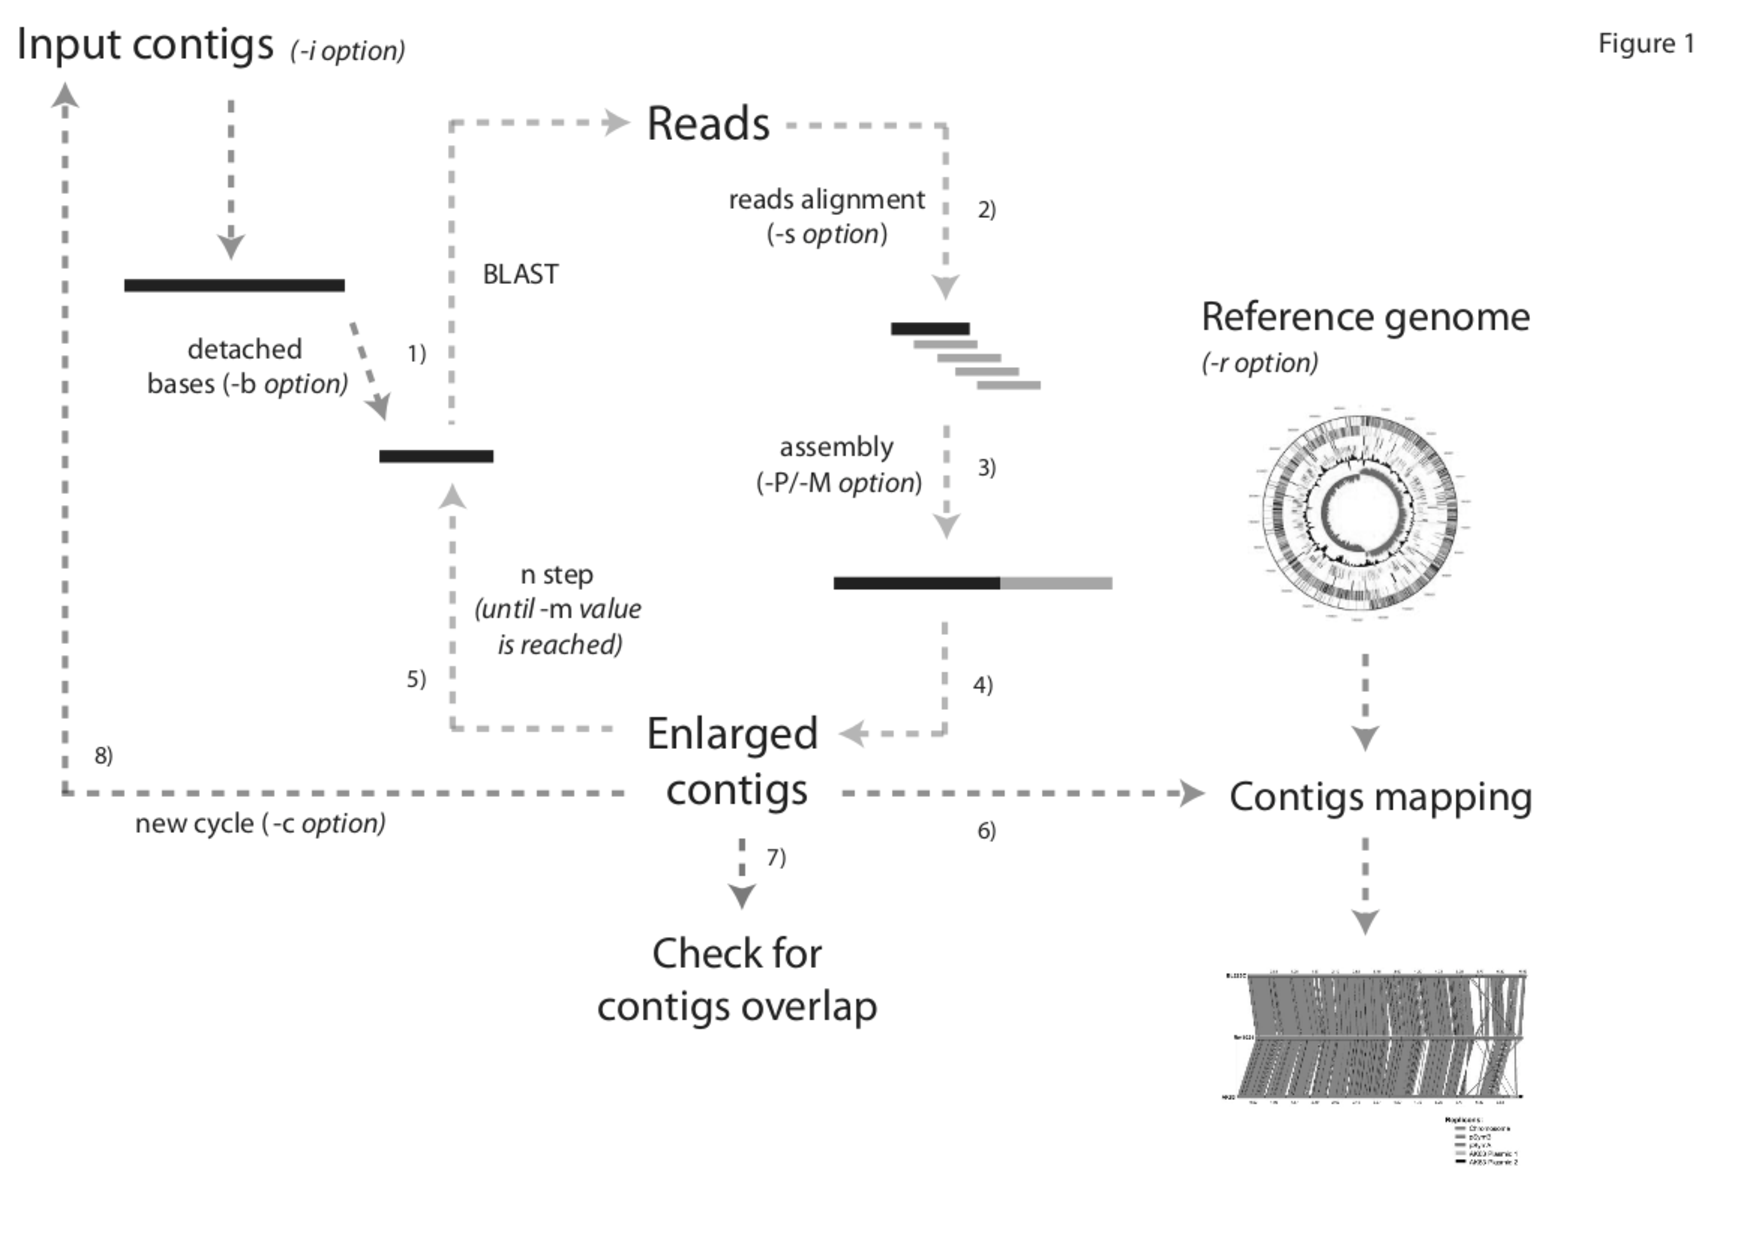
\includegraphics[width=1\textwidth]{figures/appendix/thesis_36}
	\caption{\label{fig:enly}\textbf{A schematic representation of the whole Enly pipeline together with the specific role of each parameter}}
\end{figure}

Enly is based on the iterative mapping of reads at the edges of contigs obtained after de novo assembly using Newbler or similar tools, characterized by the qualitative trimming of the contig extremities during the assembly. Enly is made up of a central core (named autoenlarge) written in C++ and by other Perl and Python modules that complete the whole pipeline (Figure \ref{fig:enly}). The computational time required for contigs extension and mapping obviously correlates with the number of contigs/reads in the input files and the number of cycles/steps (see below) specified by the user. The computational time on a machine with eight 3.1 GHz processors for the tests performed in this work (see below) ranged from 2 hours for the smallest dataset to 5 hours for the largest.
The overall procedure requires (at least) two multi-fasta files as input, one containing all the contigs deriving from the first assembly and the other all the raw reads resulting from the sequencing run. By applying the strategy described below to each contig in the input file, Enly tries to increase their length and (possibly) to merge them into scaffolds.
More in detail, the pipeline is based on the iteration of multiple cycles (Figure \ref{fig:enly}) and during each of them:
\begin{enumerate}
\item A fragment of length l1 (specified by the user) is detached from the 5’-end of each contig and is used as an input for a BLAST search \cite{camacho2009blast+} against a database embedding all the raw reads resulting from the sequencing run;
\item The BLAST output is parsed to identify reads that can be used to extend the contig (i.e. those partially aligned at the end of the contig and protruding from its extremity);
\item The identified reads and the original contig are assembled together using either Phrap \cite{machado2011phred} or Minimo \cite{treangen2011next} assemblers, possibly resulting in an “enlarged” contig (i.e. contig of increased length);
\item The very same procedure is repeated for the 3’-end of the contig and for all the other contigs of the input file;
\item The extended contigs are used as inputs for a second step, in which a fragment of length l2 (with l2< l1) is detached from each contig end and used as an input for a further BLAST against the reads database, assembling the matching reads with the enlarged contig. This procedure, performed in order to compensate for the presence of reads with a heterogeneous length distribution (resulting from a typical 454 run \cite{margulies2005genome}), is repeated for fragments of decreasing length, until the minimum length (specified by the user) has been reached;
\item If a reference genome (in fasta format) has been provided by the user, the contigs are mapped onto it, taking advantage of an ad hoc modified version of the CONTIGuator tool \cite{galardini2011contiguator};
\item When all the contigs have been processed through these steps, they are mapped one against each other for determining the eventual overlap and the closure of previously present gaps.
\end{enumerate}
The first cycle of the Enly pipeline is completed when all the contigs have been processed, mapped and saved to a new multi-fasta file. The procedure is then repeated (re-starting from point 1) for a user-specified number of cycles or, alternatively, until no more bases have been added to the contigs during the last cycle. Output files from the mapping procedure are saved in separate folders (one per cycle), ready for being loaded by the Artemis Comparison Tool \cite{carver2005act} in order to check the presence of eventual mis-assemblies.

To evaluate the reliability of the pipeline, we tested Enly on three different 454 reads datasets retrieved from either the NCBI short read archive database (SRA, \href{http://www.ncbi.nlm.nih.gov/sra}{http://www.ncbi.nlm.nih.gov/sra}), namely \textit{Escherichia coli} KO11 (SRS084754), \textit{Staphylococcus aureus} 649 (SRS114535) or from a previous sequencing run on \textit{Streptococcus pneumoniae} AP200 \cite{romina11complete}. For these reads datasets the corresponding complete genomes (E. coli KO11 and \textit{S. pneumoniae} AP200 \cite{romina11complete}\cite{turner2012optical}) or the genome of a phylogenetically close bacterium (\textit{S. aureus} COL \cite{gill2005insights}) were available, allowing the validation of the results obtained with Enly. Each reads dataset was first assembled with Newbler v. 2.6, using default parameters, resulting in 719, 254 and 124 contigs for \textit{E. coli} KO11, \textit{S. aureus} 649 and \textit{S. pneumoniae} AP200, respectively. Contigs obtained from de novo assembly were then used, together with the corresponding reads, as input for the Enly pipeline.

\begin{sidewaystable}[htbp]
  \centering
    \begin{tabular}{rrrrrrr}
    \toprule
    Strain name & Genome size (Mb) & N.  reads & Av. reads length & N.contigs & Added bases & Closed gaps \\
    \midrule
    \multicolumn{1}{c}{KO11} & \multicolumn{1}{c}{4.92} & \multicolumn{1}{c}{339,22} & \multicolumn{1}{c}{215.7} & \multicolumn{1}{c}{719} & \multicolumn{1}{c}{51,288} & \multicolumn{1}{c}{54(7.5 \%)} \\
    \multicolumn{1}{c}{649} & \multicolumn{1}{c}{2.80} & \multicolumn{1}{c}{122,569} & \multicolumn{1}{c}{245.6} & \multicolumn{1}{c}{254} & \multicolumn{1}{c}{32,446} & \multicolumn{1}{c}{27(10.6\%)} \\
    \multicolumn{1}{c}{AP200} & \multicolumn{1}{c}{2.13*} & \multicolumn{1}{c}{152,452} & \multicolumn{1}{c}{231.2} & \multicolumn{1}{c}{124} & \multicolumn{1}{c}{29,798} & \multicolumn{1}{c}{12(9.6\%)} \\
    \bottomrule
    \end{tabular}%
  \caption{\textbf{Enly results on three different reads dataset}\\
  		Enly performances after one cycle on three different 454 reads datasets, \textit{E. coli} KO11, \textit{S. aureus} 649 and \textit{S. pneumoniae} AP200. Percentages in parentheses indicate the relative number of closed gaps in respect to the ones originally present in the draft genome}
  \label{tab:enly}%
\end{sidewaystable}%

In all cases, Enly was able to improve the de novo assembly (Table \ref{tab:enly}). In particular, 12, 27 and 54 gaps were closed after one cycle of Enly, on \textit{S. pneumoniae} AP200, \textit{S. aureus} 649 and \textit{E. coli} KO11 contigs, respectively, and representing about 10\% of the gaps originally present in the draft genomes. Notably, a large amount of sequence was added to the de novo assemblies, ranging from more than 50000 bases in the cases of \textit{E. coli} KO11 to roughly 30000 in the cases of \textit{S.aureus} 649 and \textit{S. pneumoniae} AP200 genomes. In order to validate Enly results (i.e. the correctness of the overlaps identified among the extended contigs), we mapped the originally assembled contigs (i.e. before using them as input for Enly) on the corresponding complete genome sequence using Mauve \cite{darling2004mauve} with default parameters. These mapping results were compared to the positioning of the Enly-derived contigs, confirming the correctness of both the extensions and the gap closures. Iterating the algorithm of Enly for more than 1 cycle, allowed assembling even more sequence to the contigs (14517, 8411 and 37966 bases to \textit{S. pneumoniae} AP200, \textit{S. aureus} 649 and \textit{E. coli} KO11, respectively), although it did not lead to the closure of novel gaps in respect to the first cycle. 
Finally, to determine the influence of reads average length on the overall performances of the pipeline, we performed a further test on a 454 reads dataset from the 3.6 Mb genome of A\textit{cinetobacter baylyi} ADP1 (SRA id: SRX001813) whose reads were characterized by an average read length of 184 bp (thus sensibly shorter in respect to the other datasets). When tested on this dataset, Enly added 72,498 bp to the draft genome, although allowing the closure of only 2 gaps (data not shown).

Commonly-used genome finishing tools typically allow the mapping of de novo contigs on a reference genome (e.g., Projector 2 \cite{van2005projector}, CONTIGuator \cite{galardini2011contiguator}, Mauve \cite{darling2004mauve}) but very few allow to extend contigs using the original reads before mapping them. Recently, two scaffolding approaches, apparently similar to the one presented here, which take advantage of the additional information that is present on a typical Illumina paired-end sequencing run \cite{boetzer2012toward}\cite{tsai2010improving} have been developed. Nevertheless, Enly does not require a paired-end sequencing, being specifically designed for single end sequencing runs. Moreover, the pipeline does not rely on the presence of a reference genome to perform contig extension. However, since the availability of a complete genome from a closely related organism may facilitate genome closure and the identification of mis-assemblies, an optional tool (based on the CONTIGuator pipeline) to map contigs on a reference genome (if any) has been added to the overall pipeline.

\subsection{Conclusions}
Enly is a simple, cross-platform and parallelizable tool allowing the improvement of draft genomes resulting from Newbler-assembled 454 high-throughput sequencing reads. It has been shown to be particularly suited for long reads (greater than 200 bp) allowing the automated closure of about 10\% of the gaps within bacterial draft genomes, thus resulting helpful during genomes finishing procedures. The software has been developed and tested to improve genome assemblies resulting from high-throughput 454 sequencing and Newbler assembler, although, in principle, it allows the use of a large variety of read types for contig extension, including those resulting from classical sequencing methods (e.g. Sanger) or hybrid datasets, embedding a mixture of reads obtained with different technologies.

\newpage
\section{The clinical success of \textit{Acinetobacter} species: genetic, metabolic and virulence attributes}
The flexibility of the analysis methods that have been implemented in the DuctApe software suite (see section \ref{sec:ductape}) is demonstrated with the comparative genomics and phenomics study on the pathogenic \textit{Acinetobacter} species: the genomic data from four \textit{Acinetobacter} strains have been combined with the complete analysis on their phenotypes, using the Phenotype Microarray plates, in order to obtain a general view on the main metabolic differences and also to give some insights on the genetic determinants of these differences.

\newpage
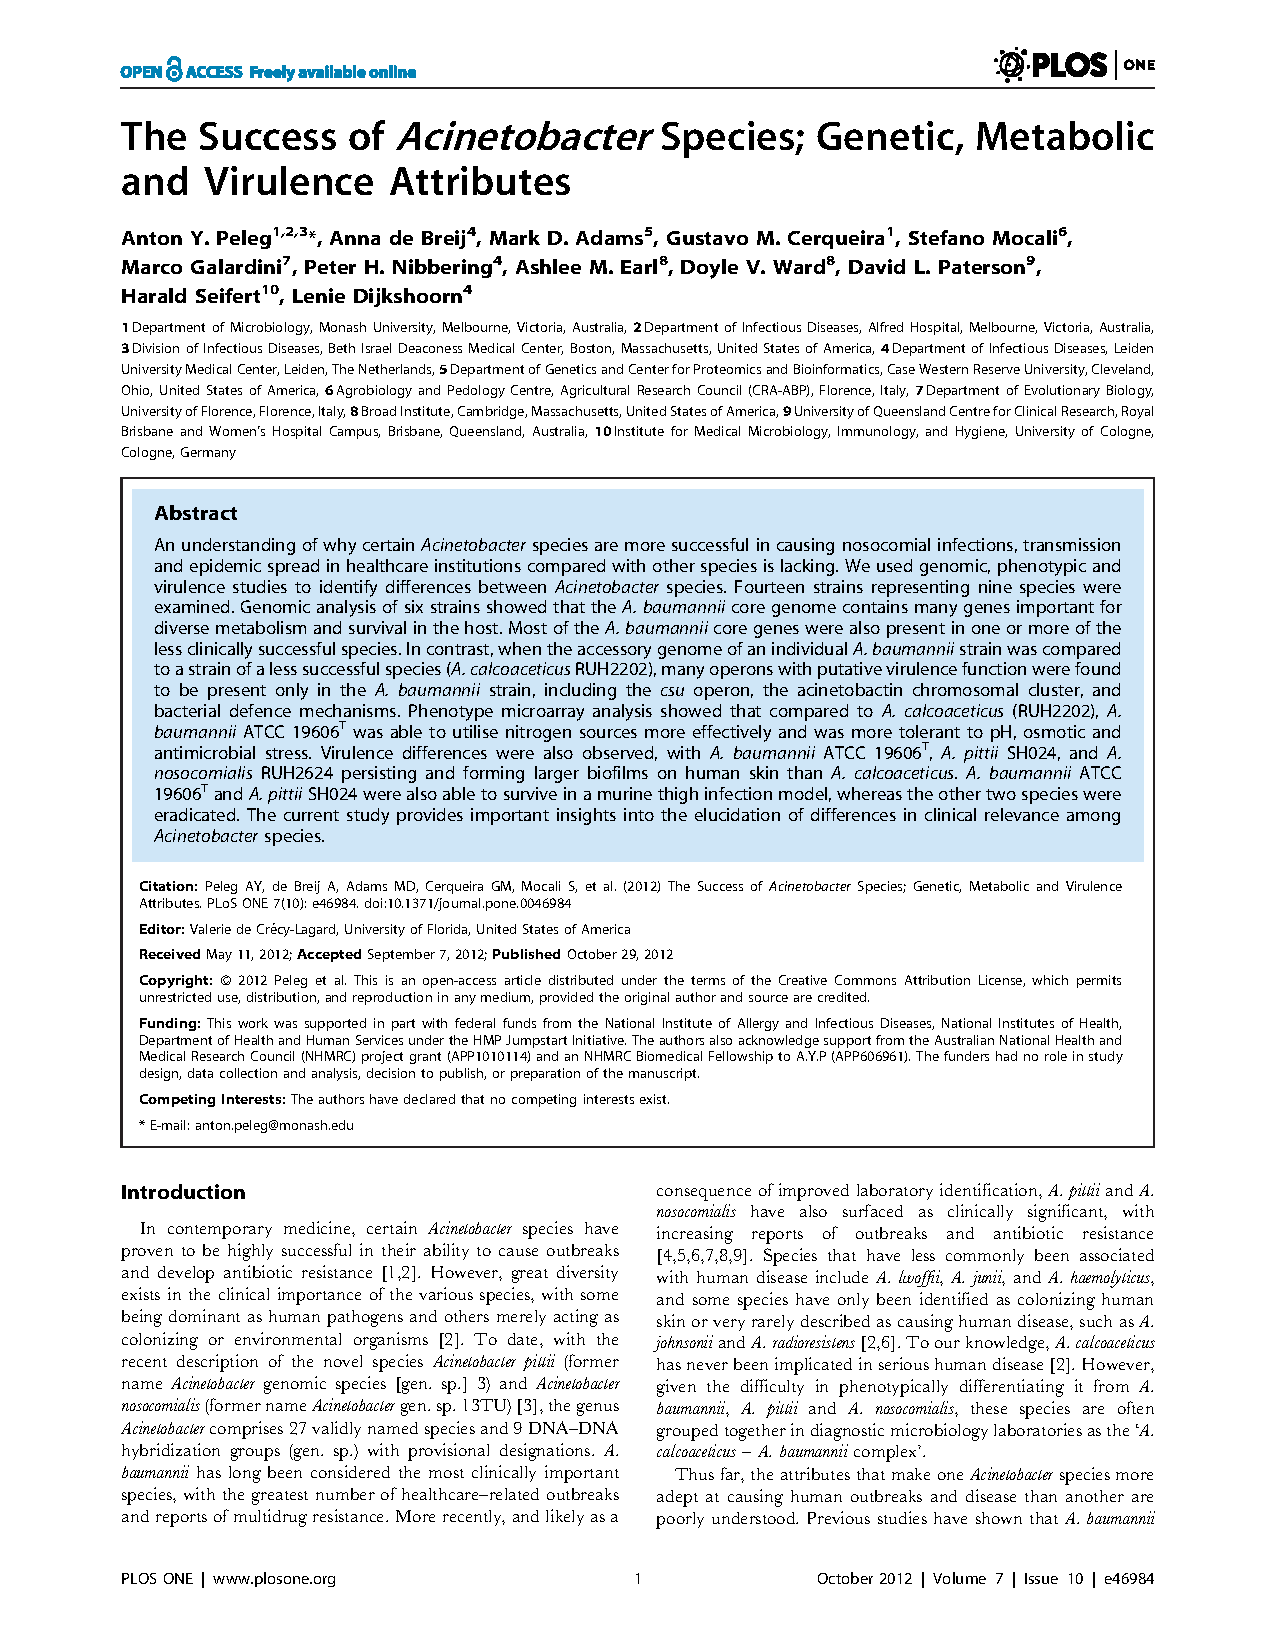
\includepdf[pages=-,offset=10mm 0, scale=0.9]{articles/Peleg2012.pdf}


%%-----------
%% Backmatter
%%-----------
\backmatter
\chaptermark{Bibliography}
\renewcommand{\sectionmark}[1]{\markright{#1}}
\bibliographystyle{unsrt}                           %Use alpha codes for references
\sectionmark{Bibliography}
\addcontentsline{toc}{chapter}{Bibliography}        %Force addition of Bibliography to TOC    
\bibliography{References}                                 %Appendix A
\mainmatter
\logvartrue
\chapter{Abreviations}

\begin{itemize}
\item \textbf{DNA}: Deoxyribonucleic acid
\item \textbf{PCR}: Polymerase Chain Reaction
\item \textbf{ORF}: Open Reading Frame
\item \textbf{ASCII}: American Standard Code for Information Interchange
\item \textbf{HMM}: Hidden Markov Model
\item \textbf{RBS}: Ribosome Binding Site
\item \textbf{BLAST}: Basic Local Alignment Search Tool
\item \textbf{KEGG}: Kyoto Encyclopedia of genes and genomes
\item \textbf{GO}: Gene Ontology
\item \textbf{COG}: Cluster of Orthologous groups
\item \textbf{LUCA}: Last Universal Common Ancestor
\item \textbf{HGT}: Horizontal Gene Transfer
\item \textbf{BBH}: Bidirectional Best Hit
\item \textbf{NGS}: Next Generation Sequencing
\item \textbf{Mb}: Megabase
\item \textbf{PCR}: Polymerase Chain Reaction
\item \textbf{dNTP}: Deoxynucleoside Triphosphate
\item \textbf{rRNA}: Ribosomial RNA
\item \textbf{PGPR}: Plant growth-promoting rhizobacteria
\item \textbf{ISR}: Induced systemic resistance
\item \textbf{BNF}: Biological nitrogen fixation
\item \textbf{ATP}: Adenosine triphosphate
\item \textbf{Mb}: Megabase
\item \textbf{CGH}: Comparative genomics hybridization
\item \textbf{API}: Application programming interface
\item \textbf{PM}: Phenotype microarray
\item \textbf{API}: Application programming interface
\item \textbf{AV}: Activity index
\item \textbf{PCA}: Principal component analysis
\end{itemize}									%Appendix B

\end{document}
% % % EOF % % %